%!TEX root = da-screen.tex

%---- Lists ----

\setenumerate{label=(\alph*)}

\newlist{descriptionb}{description}{1}
\setlist[descriptionb]{font=\normalfont\itshape,leftmargin=0pt,itemsep=1ex,style=unboxed}

\newlist{notation}{description}{1}
\setlist[notation]{font=\normalfont,labelindent=0em,leftmargin=6em,itemsep=0ex,style=sameline}

\newlist{algorithms}{description}{1}
\setlist[algorithms]{font=\normalfont,labelindent=0em,leftmargin=6em,itemsep=0ex,style=sameline}

\newlist{subex}{enumerate}{1}
\setlist[subex]{label=(\alph*),itemsep=0.25ex}

\newcommand{\algtoprule}{\rule{\columnwidth}{\heavyrulewidth}{}}
\newcommand{\algbottomrule}{\rule[1ex]{\columnwidth}{\heavyrulewidth}{}}

%---- Theorems ----

\newtheorem{theorem}{Theorem}[chapter]
\newtheorem{lemma}[theorem]{Lemma}
\newtheorem{corollary}[theorem]{Corollary}

\theoremstyle{definition}
\newtheorem{ex}{Exercise}[chapter]

%---- Notation ----

\DeclareMathOperator{\ball}{ball}
\DeclareMathOperator{\diam}{diam}
\DeclareMathOperator{\dist}{dist}
\DeclareMathOperator{\outdegree}{outdegree}
\DeclareMathOperator{\indegree}{indegree}

\DeclareMathOperator{\Input}{Input}
\DeclareMathOperator{\Output}{Output}
\DeclareMathOperator{\States}{States}
\DeclareMathOperator{\Msg}{Msg}
\DeclareMathOperator{\Init}{init}
\DeclareMathOperator{\Send}{send}
\DeclareMathOperator{\Receive}{receive}
\DeclareMathOperator{\Id}{id}

\renewcommand{\emptyset}{\varnothing}
\newcommand{\calF}{\mathcal{F}}
\newcommand{\calS}{\mathcal{S}}
\newcommand{\NN}{\mathbb{N}}
\newcommand{\RR}{\mathbb{R}}

\newcommand{\algo}[1]{\textsf{#1}}
\newcommand{\state}[1]{\textsf{\small #1}}
\newcommand{\msg}[1]{`\emph{#1}'}
\newcommand{\bin}[1]{\langle #1 \rangle}

%---- Macros ----

\newcommand{\Set}[1]{\{\, #1 \,\}}
\newcommand{\bigSet}[1]{\bigl\{\, #1 \,\bigr\}}
\newcommand{\Apx}[1]{$#1$\hyp approximation}
\newcommand{\Fact}[1]{$#1$\hyp factorisation}
\newcommand{\Reg}[1]{$#1$-regular}
\newcommand{\Dpocol}{$(\Delta+\nobreak 1)$-colouring}
\newcommand{\hint}[1]{\par\emph{Hint:} #1\par}
\newcommand{\mydash}{ --- }
\newcommand{\mysep}{\begin{center}$* \quad * \quad *$\end{center}}

%---- Figures ----

\newcounter{myexternalpagenum}
\newcommand{\definepage}[1]{\stepcounter{myexternalpagenum}\edef#1{\arabic{myexternalpagenum}}}
\definepage{\PGraph}
\definepage{\PWalk}
\definepage{\PCycle}
\definepage{\PNeighbourhood}
\definepage{\PIndependentSet}
\definepage{\PPackingCovering}
\definepage{\PPartitions}
\definepage{\PFactorisation}
\definepage{\PPnnA}
\definepage{\PPnnB}
\definepage{\PPnnC}
\definepage{\PPnnD}
\definepage{\PMaximalMatching}
\definepage{\PVCThreeApx}
\definepage{\PVCThreeApxB}
\definepage{\PVCThreeApxC}
\definepage{\PPnnTwoNode}
\definepage{\PCoveringMap}
\definepage{\PCoveringMapB}
\definepage{\PCoveringMapC}
\definepage{\PThreeReg}
\definepage{\PCyclesAndCovers}
\definepage{\PTwoEdgeCol}
\definepage{\PPathSameNeigh}
\definepage{\PSameNeigh}
\definepage{\PCoverExFourReg}
\definepage{\PCoverExThreeReg}
\definepage{\PCoverExThreeRegSpoiler}
\definepage{\PCoverExThreeRegB}
\definepage{\PNeighEx}
\definepage{\PMep}
\definepage{\PMepB}
\definepage{\PHalfSaturating}
\definepage{\PHalfSaturatingB}
\definepage{\PHalfSaturatingC}
\definepage{\PUniqueIds}
\definepage{\PGather}
\definepage{\PGreedy}
\definepage{\PDP}
\definepage{\PDPSuccessor}
\definepage{\PDPGreedy}
\definepage{\PDPCritical}
\definepage{\PIdOrient}
\definepage{\PIdPickClass}
\definepage{\PMergeColours}
\definepage{\PDirectedCycle}
\definepage{\PRtoGPart}
\definepage{\PSubsetCycle}
\definepage{\PColourLB}
\definepage{\PIntroTopo}
\definepage{\PIntroCol}
\definepage{\PIntroColTwo}
\definepage{\PIntroDegOne}
\definepage{\PIntroDegTwo}
\definepage{\PIntroTwo}
\definepage{\PIntroId}
\definepage{\PIntroIdA}
\definepage{\PIntroIdAA}
\definepage{\PIntroIdB}
\definepage{\PIntroIdBB}
\definepage{\PIntroIdC}
\definepage{\PIntroIdCC}
\definepage{\PIntroIdD}
\definepage{\PIntroIdDD}
\definepage{\PIntroIdE}
\definepage{\PIntroIdEE}
\definepage{\PIntroIdBad}
\definepage{\PIntroIdDir}
\definepage{\PIntroMis}
\definepage{\PIntroIdX}
\definepage{\PIntroTA}
\definepage{\PIntroTB}
\definepage{\PIntroTC}
\definepage{\PIntroTD}
\definepage{\PIntroTDB}
\definepage{\PIntroTwoColA}
\definepage{\PIntroTwoColB}
\definepage{\PIntroLbTwoA}
\definepage{\PIntroLbTwoB}
\definepage{\PIntroLbTwoC}
\definepage{\PIntroLbTwoD}
\definepage{\PIntroLbTwoE}


\hyphenation{auton-o-mous Hir-vo-nen Ju-ho Hir-vo-nen Kaa-si-nen Suo-me-la Tuo-mo Wawr-zyniak Ya-ma-shi-ta}

%---- Front matter ----

\title{Distributed Algorithms}
\author{Jukka Suomela}

\hypersetup{
    pdftitle={Distributed Algorithms},
    pdfauthor={Jukka Suomela},
}

\begin{document}

\frontmatter
\maketitle
\tableofcontents

\chapter*{Foreword}

This online textbook is an introduction to the theory of distributed algorithms. The topics covered in this course include algorithmic techniques that can be used to solve graph problems efficiently in extremely large networks, as well as fundamental impossibility results that put limitations on distributed computing.

No prior knowledge of distributed systems is needed. A basic knowledge of discrete mathematics and graph theory is assumed, as well as familiarity with the basic concepts from undergraduate-level courses on models on computation, computational complexity, and algorithms and data structures.

\paragraph{About the Course.}

This textbook is written to support the lecture course \emph{ICS-E5020 Distributed Algorithms} at Aalto University. The course is worth 5 ETCS credits. There are 12 weeks of lectures: each week there is one 2-hour lecture and one 2-hour exercise session. Each week we will cover roughly one section of this book.

Prior versions of this textbook have been used at the course \emph{Deterministic Distributed Algorithms}, which I lectured at the University of Helsinki in 2010, 2012, and 2014.

\paragraph{Acknowledgements.}

Many thanks to Mika G\"o\"os, Juho Hirvonen, Tee\-mu Kuu\-sisto, Tuo\-mo Lem\-pi\"a\-inen, and Jussi V\"ai\-s\"a\-nen for comments, and to Juho Hirvonen, Joel Kaasinen, and Joel Rybicki for helping me with the arrangements of this course. This work was supported in part by the Academy of Finland, Grant 252018. For updates and additional material, see
\begin{center}
    \url{http://users.ics.aalto.fi/suomela/da/}
\end{center}

\paragraph{License.}

This work is licensed under the \emph{Creative Commons Attribution--ShareAlike 3.0 Unported License}. To view a copy of this license, visit
\begin{center}
    \url{http://creativecommons.org/licenses/by-sa/3.0/}
\end{center}

\mainmatter
\chapter{Introduction and Preliminaries}

\section{Scope}

This course focuses on the \emph{theoretical foundations of distributed systems}. Our approach is similar to typical courses on models of computation, computational complexity, and design and analysis of algorithms. The main difference is in the models of computation that we study: instead of traditional models, such as finite state machines, Turing machines, RAM machines, or Boolean circuits, our model of choice is a \emph{distributed system}.

\subsection{Distributed Systems as a Model of Computation}\label{ssec:prelim-model}

A distributed system consists of multiple machines that are connected to each other through communication links. We usually view a distributed system as a (simple, undirected) graph $G = (V,E)$: each node $v \in V$ represents a machine and an edge $\{u,v\} \in E$ represents a communication link between machines $u$ and~$v$.

To understand the key difference between distributed systems and more familiar models of computation, let us consider an illustrative example: the problem of finding a maximal independent set.

An \emph{independent set} for a graph $G = (V,E)$ is a set $I \subseteq V$ such that for each edge $\{u,v\} \in E$ at most one of $u$ and $v$ is in $I$. An independent set $I$ is \emph{maximal} if it cannot be extended, i.e., it is not a proper subset of another independent set.
\begin{center}
    \includegraphics[page=\PIndependentSet]{figs.pdf}
\end{center}

Now given any model of computation $X$ we can pose the familiar question:
\begin{itemize}
    \item \emph{Computability:} is it \emph{possible} to find a maximal independent set in model $X$?
    \item \emph{Computational complexity:} can we find a maximal independent set \emph{efficiently} in model $X$?
\end{itemize}
We are familiar with such questions in the context of Turing machines, but it is not immediately obvious what these questions mean in the context of distributed systems. The following informal comparison illustrates the key differences.
\begin{description}
    \item[Input.] The input is a graph~$G$.
    \begin{descriptionb}
        \item[Turing machines:] We assume that the structure of $G$ is encoded as a string and given to the Turing machine on the input tape.
        \item[Distributed systems:] We assume that the structure of the input graph $G$ is the same as the structure of the distributed system. Initially, each machine $v \in V$ only knows some local information related to $v$ (for example, the degree of $v$ and the unique identifier of $v$). To acquire more information about $G$, the nodes need to exchange messages.
    \end{descriptionb}
    \item[Output.] The output is an independent set $I \subseteq V$.
    \begin{descriptionb}
        \item[Turing machines:] We require that the machine prints an encoding of $I$ on the output tape.
        \item[Distributed systems:] We require that each node $v \in V$ produces one bit of output: if $v \in I$, node $v$ has to output $1$, and if $v \notin I$, node $v$ has to output $0$.
    \end{descriptionb}
    \item[Algorithm.] We say that an algorithm solves the problem if it produces a valid output for any valid input.
    \begin{descriptionb}
        \item[Turing machines:] The algorithm designer chooses the state transitions of the Turing machine.
        \item[Distributed systems:] The algorithm designer writes one program. The same program is installed in each $v \in V$.
    \end{descriptionb}
    \item[Complexity measures.] There are many possible complexity measures, but perhaps the most commonly used is the time complexity.
    \begin{descriptionb}
        \item[Turing machines:] Time = number of elementary steps. In each time unit, (1)~the machine moves the tape heads, (2)~performs a state transition that depends on the contents of the tapes, and (3)~possibly halts.
        \item[Distributed systems:] Time = number of synchronous communication rounds. In each time unit, all machines in parallel (1)~exchange messages with their neighbours, (2)~perform state transitions that depend on the messages that they received, and (3)~possibly halt.
    \end{descriptionb}
\end{description}
To oversimplify a bit, distributed computation is not really about \emph{computation}\mydash it is all about \emph{communication}. Throughout this course, we will see striking examples of the implications of this change of perspective.


\subsection{Outside the Scope}

The term ``distributed computing'' is overloaded, and it means very different things to different people.

For the general public, distributed computing often refers to large-scale high-performance computing in a computer network; this includes scientific computing on grids and clusters, and volunteer computing projects such as SETI@Home and Folding@Home. However, this is \emph{not} the definition that we use, and our course is in no way related to large-scale number crunching.

In general, our focus is on theory, not practice. For our purposes, a communication network is an idealised abstraction. We are not interested in any implementation details or engineering aspects. For example, the following topics are \emph{not} covered on this course: physical properties of wired or wireless media, modulation techniques, communication protocols, standards, software architectures, programming languages, software libraries, privacy, and security.

Within the field of the theory of distributed computing, there are also numerous topics that we are not going to cover. We will conclude this course with a brief overview of other research areas within the field in Section~\ref{sec:other-stuff}.


\section{Graphs}\label{sec:graphs}

As we already saw in Section~\ref{ssec:prelim-model}, the study of distributed algorithms is closely related to graphs: we will interpret a computer network as a graph, and we will study computational problems related to this graph. In this section we will give a summary of graph-theoretic concepts that we will use.

\subsection{Terminology}

A \emph{simple undirected graph} is a pair $G = (V,E)$, where $V$ is the set of \emph{nodes} (\emph{vertices}) and $E$ is the set of \emph{edges}. Each edge $e \in E$ is a 2-subset of nodes, that is, $e = \{u,v\}$ where $u \in V$, $v \in V$, and $u \ne v$. Unless otherwise mentioned, we assume that $V$ is a non-empty finite set; it follows that $E$ is a finite set. Usually, we will draw graphs using circles and lines\mydash each circle represents a node, and a line that connects two nodes represents an edge.

\paragraph{Adjacency.}

If $e = \{u,v\} \in E$, we say that node $u$ is \emph{adjacent} to $v$, nodes $u$ and $v$ are \emph{neighbours}, node $u$ is \emph{incident} to $e$, and edge $e$ is also \emph{incident} to $u$. If $e_1, e_2 \in E$, $e_1 \ne e_2$, and $e_1 \cap e_2 \ne \emptyset$ (i.e., $e_1$ and $e_2$ are distinct edges that share an endpoint), we say that $e_1$ is \emph{adjacent} to $e_2$.
\begin{figure}
    \centering
    \includegraphics[page=\PGraph]{figs.pdf}
    \caption{Node $u$ is adjacent to node $v$. Nodes $u$ and $v$ are incident to edge $e$. Edge $e_1$ is adjacent to edge $e_2$.}\label{fig:graph}
\end{figure}

The \emph{degree} of a node $v \in V$ in graph $G$ is \[
    \deg_G(v) = \bigl|\bigSet{ u \in V : \{u,v\} \in E }\bigr|.
\]
That is, $v$ has $\deg_G(v)$ neighbours; it is adjacent to $\deg_G(v)$ nodes and incident to $\deg_G(v)$ edges. A node $v \in V$ is \emph{isolated} if $\deg_G(v) = 0$. Graph $G$ is \emph{\Reg{k}} if $\deg_G(v) = k$ for each $v \in V$.

\paragraph{Subgraphs.}

Let $G = (V,E)$ and $H = (V_2,E_2)$ be two graphs. If $V_2 \subseteq V$ and $E_2 \subseteq E$, we say that $H$ is a \emph{subgraph} of $G$. If $V_2 = V$, we say that $H$ is a \emph{spanning subgraph} of $G$.

If $V_2 \subseteq V$ and $E_2 = \Set{ \{u,v\} \in E : u \in V_2,\ v \in V_2 }$, we say that $H = (V_2,E_2)$ is an \emph{induced subgraph}; more specifically, $H$ is the subgraph of $G$ induced by nodes $V_2$.

If $E_2 \subseteq E$ and $V_2 = \bigcup E_2$, we say that $H$ is an \emph{edge-induced subgraph}; more specifically, $H$ is the subgraph of $G$ induced by edges $E_2$.

\paragraph{Walks.}

\begin{figure}
    \centering
    \includegraphics[page=\PWalk]{figs.pdf}
    \caption{
        (a)~A walk of length~5 from $s$ to $t$.
        (b)~A non-backtracking walk.
        (c)~A path of length~4.
        (d)~A path of length~2; this is a shortest path and hence $\dist_G(s,t) = 2$.
    }\label{fig:walk}
\end{figure}

\begin{figure}
    \centering
    \includegraphics[page=\PCycle]{figs.pdf}
    \caption{
        (a)~A cycle of length~6.
        (b)~A cycle of length~3; this is a shortest cycle and hence the girth of the graph is~$3$.
    }\label{fig:cycle}
\end{figure}

A \emph{walk} of length $\ell$ from node $v_0$ to node $v_\ell$ is an alternating sequence $w = (v_0, e_1, v_1, e_2, v_2, \dotsc, e_\ell, v_\ell)$ where $v_i \in V$, $e_i \in E$, and $e_i = \{ v_{i-1}, v_i \}$ for all $i$; see Figure~\ref{fig:walk}. The walk is \emph{empty} if $\ell = 0$. We say that walk~$w$ \emph{visits} the nodes $v_0, v_1, \dotsc, v_\ell$, and it \emph{traverses} the edges $e_1, e_2, \dotsc, e_\ell$. In general, a walk may visit the same node more than once and it may traverse the same edge more than once. A \emph{non-backtracking walk} does not traverse the same edge twice consecutively, that is, $e_{i-1} \ne e_i$ for all $i$. A \emph{path} is a walk that visits each node at most once, that is, $v_i \ne v_j$ for all $0 \le i < j \le \ell$. A walk is \emph{closed} if $v_0 = v_\ell$. A \emph{cycle} is a non-empty closed walk with $v_i \ne v_j$ and $e_i \ne e_j$ for all $1 \le i < j \le \ell$; it follows that the length of a cycle is at least~$3$.

\paragraph{Connectivity and Distances.}

For each graph $G = (V,E)$, we can define a relation $\leadsto$ on $V$ as follows: $u \leadsto v$ if there is a walk from $u$ to $v$. Clearly $\leadsto$ is an equivalence relation. Let $C \subseteq V$ be an equivalence class; the subgraph induced by $C$ is called a \emph{connected component} of $G$.

If $u$ and $v$ are in the same connected component, there is at least one \emph{shortest path} from $u$ to $v$, that is, a path from $u$ to $v$ of the smallest possible length. Let $\ell$ be the length of a shortest path from $u$ to $v$; we define that the \emph{distance} between $u$ and $v$ in $G$ is $\dist_G(u,v) = \ell$. If $u$ and $v$ are not in the same connected component, we define $\dist_G(u,v) = \infty$. Note that $\dist_G(u,u) = 0$ for any node $u$.

\begin{figure}
    \centering
    \includegraphics[page=\PNeighbourhood]{figs.pdf}
    \caption{Neighbourhoods.}\label{fig:neighbourhood}
\end{figure}
For each node $v$ and for a non-negative integer $r$, we define the \emph{radius-$r$ neighbourhood} of $v$ as follows:
\[
    \ball_G(v, r) = \Set{ u \in V : \dist_G(u,v) \le r }.
\]

A graph is \emph{connected} if it consists of one connected component. The \emph{diameter} of graph $G$, in notation $\diam(G)$, is the length of a longest shortest path, that is, the maximum of $\dist_G(u,v)$ over all $u, v \in V$; we have $\diam(G) = \infty$ if the graph is not connected.

The \emph{girth} of graph $G$ is the length of a shortest cycle in $G$. If the graph does not have any cycles, we define that the girth is $\infty$; in that case we say that $G$ is \emph{acyclic}.

A \emph{tree} is a connected, acyclic graph. If $T = (V,E)$ is a tree and $u,v \in V$, then there exists precisely one path from $u$ to $v$. An acyclic graph is also known as a \emph{forest}\mydash in a forest each connected component is a tree. A \emph{pseudotree} has at most one cycle, and in a \emph{pseudoforest} each connected component is a pseudotree.

A \emph{path graph} is a graph that consists of one path, and a \emph{cycle graph} is a graph that consists of one cycle. Put otherwise, a path graph is a tree in which all nodes have degree at most $2$, and a cycle graph is a \Reg{2} pseudotree. Note that any graph of maximum degree $2$ consists of disjoint paths and cycles, and any \Reg{2} graph consists of disjoint cycles.

\paragraph{Isomorphism.}

An \emph{isomorphism} from graph $G_1 = (V_1,E_1)$ to graph $G_2 = (V_2,E_2)$ is a bijection $f\colon V_1 \to V_2$ that preserves adjacency: $\{u,v\} \in E_1$ if and only if $\{f(u),f(v)\} \in E_2$. If an isomorphism from $G_1$ to $G_2$ exists, we say that $G_1$ and $G_2$ are isomorphic.

If $G_1$ and $G_2$ are isomorphic, they have the same structure; informally, $G_2$ can be constructed by renaming the nodes of $G_1$ and vice versa.


\subsection{Packing and Covering}\label{ssec:packingcovering}

A subset of nodes $X \subseteq V$ is
\begin{enumerate}
    \item an \emph{independent set} if each edge has at most one endpoint in $X$, that is, $|e \cap X| \le 1$ for all $e \in E$,
    \item a \emph{vertex cover} if each edge has at least one endpoint in $X$, that is, $e \cap X \ne \emptyset$ for all $e \in E$,
    \item a \emph{dominating set} if each node $v \notin X$ has at least one neighbour in $X$, that is, $\ball_G(v,1) \cap X \ne \emptyset$ for all $v \in V$.
\end{enumerate}
A subset of edges $X \subseteq E$ is
\begin{enumerate}[resume]
    \item a \emph{matching} if each node has at most one incident edge in $X$, that is, $\{t,u\} \in X$ and $\{t,v\} \in X$ implies $u = v$,
    \item an \emph{edge cover} if each node has at least one incident edge in $X$, that is, $\bigcup X = V$,
    \item an \emph{edge dominating set} if each edge $e \notin X$ has at least one neighbour in $X$, that is, $e \cap \bigl(\bigcup X\bigr) \ne \emptyset$ for all $e \in E$.
\end{enumerate}
See Figure~\ref{fig:packingcovering} for illustrations.
\begin{figure}
    \centering
    \includegraphics[page=\PPackingCovering]{figs.pdf}
    \caption{Packing and covering problems; see Section~\ref{ssec:packingcovering}.}\label{fig:packingcovering}
\end{figure}

Independent sets and matchings are examples of \emph{packing problems}\mydash intuitively, we have to ``pack'' elements into set $X$ while avoiding conflicts. Packing problems are \emph{maximisation problems}. Typically, it is trivial to find a feasible solution (for example, an empty set), but it is more challenging to find a large solution.

Vertex covers, edge covers, dominating sets, and edge dominating sets are examples of \emph{covering problems}\mydash intuitively, we have to find a set $X$ that ``covers'' the relevant parts of the graph. Covering problems are \emph{minimisation problems}. Typically, it is trivial to find a feasible solution if it exists (for example, the set of all nodes or all edges), but it is more challenging to find a small solution.

The following terms are commonly used in the context of maximisation problems; it is important not to confuse them:
\begin{enumerate}
    \item \emph{maximal}: a maximal solution is not a proper subset of another feasible solution,
    \item \emph{maximum}: a maximum solution is a solution of the largest possible cardinality.
\end{enumerate}
Similarly, in the context of minimisation problems, analogous terms are used:
\begin{enumerate}
    \item \emph{minimal}: a minimal solution is not a proper superset of another feasible solution,
    \item \emph{minimum}: a minimum solution is a solution of the smallest possible cardinality.
\end{enumerate}
Using this convention, we can define the terms \emph{maximal independent set}, \emph{maximum independent set}, \emph{maximal matching}, \emph{maximum matching}, \emph{minimal vertex cover}, \emph{minimum vertex cover}, etc.

For example, Figure~\ref{fig:packingcovering}a shows a maximal independent set: it is not possible to greedily extend the set by adding another element. However, it is not a maximum independent set: there exists an independent set of size $3$. Figure~\ref{fig:packingcovering}d shows a matching, but it is not a maximal matching, and therefore it is not a maximum matching either.

Typically, maximal and minimal solutions are easy to find\mydash you can apply a greedy algorithm. However, maximum and minimum solutions can be very difficult to find\mydash many of these problems are NP-hard optimisation problems.

A \emph{minimum maximal matching} is precisely what the name suggests: it is a maximal matching of the smallest possible cardinality. We can define a \emph{minimum maximal independent set}, etc., in an analogous manner.


\subsection{Labellings and Partitions}\label{ssec:partitions}

We will often encounter functions of the form \[f\colon V \to \{1,2,\dotsc,k\}.\] There are two interpretations that are often helpful:
\begin{enumerate}[label=(\roman*)]
    \item Function $f$ assigns a \emph{label} $f(v)$ to each node $v \in V$. Depending on the context, the labels can be interpreted as colours, time slots, etc.
    \item Function $f$ is a \emph{partition} of $V$. More specifically, $f$ defines a partition $V = V_1 \cup V_2 \cup \dotsb \cup V_k$ where $V_i = f^{-1}(i) = \Set{ v \in V : f(v) = i }$.
\end{enumerate}
Similarly, we can study a function of the form \[f\colon E \to \{1,2,\dotsc,k\}\] and interpret it either as a labelling of edges or as a partition of~$E$.

Many graph problems are related to such functions. We say that a function $f\colon V \to \{1,2,\dotsc,k\}$ is
\begin{enumerate}
    \item a \emph{proper vertex colouring} if $f^{-1}(i)$ is an independent set for each~$i$,
    \item a \emph{weak colouring} if each non-isolated node $u$ has a neighbour $v$ with $f(u) \ne f(v)$,
    \item a \emph{domatic partition} if $f^{-1}(i)$ is a dominating set for each~$i$.
\end{enumerate}
A function $f\colon E \to \{1,2,\dotsc,k\}$ is
\begin{enumerate}[resume]
    \item a \emph{proper edge colouring} if $f^{-1}(i)$ is a matching for each~$i$,
    \item an \emph{edge domatic partition} if $f^{-1}(i)$ is an edge dominating set for each~$i$.
\end{enumerate}
See Figure~\ref{fig:partitions} for illustrations.
\begin{figure}
    \centering
    \includegraphics[page=\PPartitions]{figs.pdf}
    \caption{Partition problems; see Section~\ref{ssec:partitions}.}\label{fig:partitions}
\end{figure}

Usually, the term \emph{colouring} refers to a proper vertex colouring, and the term \emph{edge colouring} refers to a proper edge colouring. The value of $k$ is the \emph{size} of the colouring or the \emph{number of colours}. We will use the term \emph{$k$-colouring} to refer to a proper vertex colouring with $k$ colours; the term \emph{$k$-edge colouring} is defined in an analogous manner.

A graph that admits a $2$-colouring is a \emph{bipartite graph}. Equivalently, a bipartite graph is a graph that does not have an odd cycle.

Graph colouring is typically interpreted as a minimisation problem. It is easy to find a proper vertex colouring or a proper edge colouring if we can use arbitrarily many colours; however, it is difficult to find an \emph{optimal} colouring that uses the smallest possible number of colours.

On the other hand, domatic partitions are a maximisation problem. It is trivial to find a domatic partition of size $1$; however, it is difficult to find an \emph{optimal} domatic partition with the largest possible number of disjoint dominating sets.


\subsection{Factors and Factorisations}

Let $G = (V,E)$ be a graph, let $X \subseteq E$ be a set of edges, and let $H = (U,X)$ be the subgraph of $G$ induced by $X$. We say that $X$ is a \emph{$d$-factor} of $G$ if $U = V$ and $\deg_H(v) = d$ for each $v \in V$.

Equivalently, $X$ is a $d$-factor if $X$ induces a spanning \Reg{d} subgraph of $G$. Put otherwise, $X$ is a $d$-factor if each node $v \in V$ is incident to exactly $d$ edges of $X$.

A function $f\colon E \to \{1,2,\dotsc,k\}$ is a \emph{\Fact{d}} of $G$ if $f^{-1}(i)$ is a $d$-factor for each $i$. See Figure~\ref{fig:factorisation} for examples.
\begin{figure}
    \centering
    \includegraphics[page=\PFactorisation]{figs.pdf}
    \caption{
        (a)~A \Fact{1} of a \Reg{3} graph.
        (b)~A \Fact{2} of a \Reg{4} graph.
    }\label{fig:factorisation}
\end{figure}

We make the following observations:
\begin{enumerate}
    \item A $1$-factor is a maximum matching. If a $1$-factor exists, a maximum matching is a $1$-factor.
    \item A \Fact{1} is an edge colouring.
    \item The subgraph induced by a $2$-factor consists of disjoint cycles.
\end{enumerate}
A $1$-factor is also known as a \emph{perfect matching}.


\subsection{Approximations}

So far we have encountered a number of maximisation problems and minimisation problems. More formally, the definition of a maximisation problem consists of two parts: a set of \emph{feasible solutions} $\calS$ and an \emph{objective function} $g\colon \calS \to \RR$. In a maximisation problem, the goal is to find a feasible solution $X \in \calS$ that maximises $g(X)$. A minimisation problem is analogous: the goal is to find a feasible solution $X \in \calS$ that minimises $g(X)$.

For example, the problem of finding a maximum matching for a graph $G$ is of this form. The set of feasible solutions $\calS$ consists of all matchings in $G$, and we simply define $g(M) = |M|$ for each matching $M \in \calS$.

As another example, the problem of finding an optimal colouring is a minimisation problem. The set of feasible solutions $\calS$ consists of all proper vertex colourings, and $g(f)$ is the number of colours in $f \in \calS$.

Often, it is infeasible or impossible to find an optimal solution; hence we resort to approximations. Given a maximisation problem $(\calS,g)$, we say that a solution $X$ is an \emph{\Apx{\alpha}} if $X \in \calS$, and we have $\alpha g(X) \ge g(Y)$ for all $Y \in \calS$. That is, $X$ is a feasible solution, and the size of $X$ is within factor $\alpha$ of the optimum.

Similarly, if $(\calS,g)$ is a minimisation problem, we say that a solution $X$ is an \Apx{\alpha} if $X \in \calS$, and we have $g(X) \le \alpha g(Y)$ for all $Y \in \calS$. That is, $X$ is a feasible solution, and the size of $X$ is within factor $\alpha$ of the optimum.

Note that we follow the convention that the approximation ratio $\alpha$ is always at least $1$, both in the case of minimisation problems and maximisation problems. Other conventions are also used in the literature.


\subsection{Directed Graphs and Orientations}

Unless otherwise mentioned, all graphs in this course are undirected. However, we will occasionally need to refer to so-called orientations, and hence we need to introduce some terminology related to directed graphs.

A \emph{directed graph} is a pair $G = (V,E)$, where $V$ is the set of nodes and $E$ is the set of \emph{directed edges}. Each edge $e \in E$ is a pair of nodes, that is, $e = (u,v)$ where $u, v \in V$. Put otherwise, $E \subseteq V \times V$.

Intuitively, an edge $(u,v)$ is an ``arrow'' that points from node $u$ to node $v$; it is an \emph{outgoing edge} for $u$ and an \emph{incoming edge} for $v$. The \emph{outdegree} of a node $v \in V$, in notation $\outdegree_G(v)$, is the number of outgoing edges, and the \emph{indegree} of the node, $\indegree_G(v)$, is the number of incoming edges.

Now let $G = (V,E)$ be a graph and let $H = (V,E')$ be a directed graph with the same set of nodes. We say that $H$ is an \emph{orientation} of $G$ if the following holds:
\begin{enumerate}
    \item For each $\{u,v\} \in E$ we have either $(u,v) \in E'$ or $(v,u) \in E'$, but not both.
    \item For each $(u,v) \in E'$ we have $\{u,v\} \in E$.
\end{enumerate}
Put otherwise, in an orientation of $G$ we have simply chosen an arbitrary direction for each undirected edge of $G$. It follows that \[\indegree_H(v) + \outdegree_H(v) = \deg_G(v)\] for all $v \in V$.


\section{Exercises}

\begin{ex}[independence and vertex covers]
    Let $I \subseteq V$ and define $C = V \setminus I$. Show that
    \begin{subex}
        \item if $I$ is an independent set then $C$ is a vertex cover and vice versa,
        \item if $I$ is a maximal independent set then $C$ is a minimal vertex cover and vice versa,
        \item if $I$ is a maximum independent set then $C$ is a minimum vertex cover and vice versa,
        \item it is possible that $C$ is a \Apx{2} of minimum vertex cover but $I$ is not a \Apx{2} of maximum independent set,
        \item it is possible that $I$ is a \Apx{2} of maximum independent set but $C$ is not a \Apx{2} of minimum vertex cover.
    \end{subex}
\end{ex}

\begin{ex}[matchings]
    Show that
    \begin{subex}
        \item any maximal matching is a \Apx{2} of a maximum matching,
        \item any maximal matching is a \Apx{2} of a minimum maximal matching,
        \item a maximal independent set is not necessarily a \Apx{2} of maximum independent set,
        \item a maximal independent set is not necessarily a \Apx{2} of minimum maximal independent set.
    \end{subex}
\end{ex}

\begin{ex}[matchings and vertex covers]\label{ex:mmvc}
    Let $M$ be a maximal matching, and let $C = \bigcup M$, i.e., $C$ consists of all endpoints of matched edges. Show that
    \begin{subex}
        \item $C$ is a \Apx{2} of a minimum vertex cover,
        \item $C$ is not necessarily a \Apx{1.999} of a minimum vertex cover.
    \end{subex}
    Would you be able to improve the approximation ratio if $M$ was a minimum maximal matching?
\end{ex}

\begin{ex}[independence and domination]
    Show that
    \begin{subex}
        \item a maximal independent set is a minimal dominating set,
        \item a minimal dominating set is not necessarily a maximal independent set,
        \item a minimum maximal independent set is not necessarily a minimum dominating set.
    \end{subex}
\end{ex}

\begin{ex}[matchings and edge domination]\label{ex:mmeds}
    Show that
    \begin{subex}
        \item a maximal matching is a minimal edge dominating set,
        \item a minimal edge dominating set is not necessarily a maximal matching,
        \item a minimum maximal matching is a minimum edge dominating set,
        \item any maximal matching is a \Apx{2} of a minimum edge dominating set.
    \end{subex}
    \hint{Assume that $D$ is an edge dominating set; show that you can construct a maximal matching $M$ with $|M| \le |D|$.}
\end{ex}

\begin{ex}[graph colourings and partitions]
    Show that
    \begin{subex}
        \item a weak $2$-colouring always exists,
        \item a domatic partition of size $2$ does not necessarily exist,
        \item if a domatic partition of size $2$ exists, then a weak $2$-colouring is a domatic partition of size $2$,
        \item a weak $2$-colouring is not necessarily a domatic partition of size $2$.
    \end{subex}
    Show that there are \Reg{2} graphs with the following properties:
    \begin{subex}[resume]
        \item any $3$-colouring is a domatic partition of size $3$,
        \item no $3$-colouring is a domatic partition of size $3$.
    \end{subex}
    Assume that $G$ is a graph of maximum degree $\Delta$; show that
    \begin{subex}[resume]
        \item there exists a \Dpocol,
        \item a $\Delta$-colouring does not necessarily exist.
    \end{subex}
\end{ex}

\begin{ex}[line graphs]
    Look up the definition of a \emph{line graph}. Whenever possible, use line graphs to explain
    \begin{subex}
        \item the connection between matchings and independent sets,
        \item the connection between dominating sets and edge dominating sets,
        \item the connection between node colourings and edge colourings.
    \end{subex}
\end{ex}

\begin{ex}[isomorphism]
    Construct non-empty \Reg{3} connected graphs $G$ and $H$ such that $G$ and $H$ have the same number of nodes and $G$ and $H$ are \emph{not} isomorphic.
\end{ex}

\begin{ex}[Petersen 1891]\label{ex:2fact}
    Show that any \Reg{2d} graph has a \Fact{2}.
\end{ex}

\begin{ex}[orientations]
    Using the result of Exercise~\ref{ex:2fact}, show that any \Reg{2d} graph $G = (V,E)$ has an orientation $H = (V,E')$ such that $\indegree_H(v) = \outdegree_H(v) = d$ for all $v \in V$.
\end{ex}


\chapter{Port-Numbering Model}

\section{Introduction}

Now that we have introduced the essential graph-theoretic concepts, we are ready to define what a ``distributed algorithm'' is. In this chapter, we will study one variant of the theme: distributed algorithm in the ``port-numbering model''. The basic idea is best explained through an example. Suppose that I claim the following:
\begin{itemize}
    \item $A$ is a deterministic distributed algorithm that finds a \Apx{2} of a minimum vertex cover in the port-numbering model.
\end{itemize}
Informally, this entails the following:
\begin{enumerate}
    \item We can take any simple undirected graph $G = (V,E)$.
    \item We can then put together a computer network $N$ with the same structure as $G$. A node $v \in V$ corresponds to a computer in $N$, and an edge $\{u,v\} \in E$ corresponds to a communication link between the computers $u$ and $v$.
    \item More precisely, a node of degree $d$ corresponds to a computer with $d$ communication ports that are labelled with numbers $1, 2, \dotsc, d$. Each port is connected to precisely one neighbour.
    \item Each computer runs a copy of the same deterministic algorithm $A$. All nodes are identical; initially they know only their own degree (i.e., the number of communication ports).
    \item All computers are started simultaneously, and they follow algorithm $A$ synchronously in parallel. In each synchronous communication round, all computers in parallel
    \begin{enumerate}[label=(\arabic*)]
        \item send a message to each of their ports,
        \item wait while the messages are propagated along the communication channels,
        \item receive a message from each of their ports, and
        \item update their own state.
    \end{enumerate}
    \item After each round, a computer can stop and announce its \emph{local output}: in this case the local output is either $0$ or $1$.
    \item We require that all nodes eventually stop\mydash the \emph{running time} of the algorithm is the number of communication rounds it takes until all nodes have stopped.
    \item We require that
        \[ C = \Set{ v \in V : \text{computer $v$ produced output $1$} } \]
        is a feasible vertex cover for graph $G$, and its size is at most $2$ times the size of a minimum vertex cover. 
\end{enumerate}
Sections \ref{sec:pnn} and \ref{sec:distr-alg} below go through the effort of formalising this idea. While at it, we also address the following issues:
\begin{enumerate}
    \item It is easy to encode a subset of nodes using local outputs\mydash but how should we encode, for example, a subset of edges?
    \item Often it is useful to have not only local outputs but also a \emph{local input} for each computer. Then we could compose algorithms: first, algorithm $A_1$ solves a problem $\Pi_1$; then algorithm $A_2$ uses the solution of $\Pi_1$ to solve a problem~$\Pi_2$.
    \item Often we will focus our attention to certain families of graphs\mydash it is too much to expect that an algorithm could solve a problem in \emph{any} undirected graph~$G$.
\end{enumerate}

\section{Port-Numbered Network}\label{sec:pnn}

A \emph{port-numbered network} is a triple $N = (V,P,p)$, where $V$ is the set of \emph{nodes}, $P$ is the set of \emph{ports}, and $p\colon P \to P$ is a function that specifies the \emph{connections} between the ports. We make the following assumptions:
\begin{enumerate}
    \item Each port is a pair $(v,i)$ where $v \in V$ and $i \in \{1,2,\dotsc\}$.
    \item The connection function $p$ is an involution, that is, for any port $x \in P$ we have $p(p(x)) = x$.
\end{enumerate}
See Figures \ref{fig:pnna} and \ref{fig:pnnb} for illustrations.
\begin{figure}
    \centering
    \includegraphics[page=\PPnnA]{figs.pdf}
    \caption{A port-numbered network $N = (V,P,p)$. There are four nodes, $V = \{a,b,c,d\}$; the degree of node $a$ is $3$, the degrees of nodes $b$ and $c$ are $2$, and the degree of node $d$ is $1$. The connection function $p$ is illustrated with arrows\mydash for example, $p(a,3) = (d,1)$ and conversely $p(d,1) = (a,3)$. This network is simple.}\label{fig:pnna}
\end{figure}
\begin{figure}
    \centering
    \includegraphics[page=\PPnnB]{figs.pdf}
    \caption{A port-numbered network $N = (V,P,p)$. There is a loop at node $a$, as $p(a,1) = (a,1)$, and another loop at node $d$, as $p(d,3) = (d,4)$. There are also multiple connections between $c$ and $d$. Hence the network is not simple.}\label{fig:pnnb}
\end{figure}

\subsection{Terminology}

If $(v,i) \in P$, we say that $(v,i)$ is the port number $i$ in node $v$. The \emph{degree} $\deg_N(v)$ of a node $v \in V$ is the number of ports in $v$, that is, $\deg_N(v) = |\Set{ i \in \NN : (v,i) \in P }|$.

Unless otherwise mentioned, we assume that the port numbers are \emph{consecutive}: for each $v \in V$ there are ports $(v,1),\allowbreak (v,2),\allowbreak \dotsc,\allowbreak (v,\deg_N(v))$ in~$P$.

If $(v,i) \in P$, we use the shorthand notation $p(v,i)$ for $p((v,i))$. If $p(u,i) = (v,j)$, we say that port $(u,i)$ is \emph{connected} to port $(v,j)$; we also say that port $(u,i)$ is connected to node $v$, and that node $u$ is connected to node~$v$.

If $p(v,i) = (v,j)$ for some $j$, we say that there is a \emph{loop} at $v$\mydash note that we may have $i = j$ or $i \ne j$. If $p(u,i_1) = (v,j_1)$ and $p(u,i_2) = (v,j_2)$ for some $u \ne v$, $i_1 \ne i_2$, and $j_1 \ne j_2$, we say that there are \emph{multiple connections} between $u$ and~$v$. A port-numbered network $N = (V,P,p)$ is \emph{simple} if there are no loops or multiple connections. 

\subsection{Intuition}

The intuitive idea behind the definition is that a simple port-numbered network $N$ is a model of a physical, real-world communication network:
\begin{enumerate}
    \item each node $v \in V$ is a physical device (e.g., a computer or a router),
    \item node $v$ has $\deg_N(v)$ communication ports, labelled with integers $1,2,\dotsc,\allowbreak\deg_N(v)$,
    \item $p(u,i) = (v,j)$ indicates that there is a cable that connects the port number $i$ in device $u$ with the port number $j$ in device $v$.
\end{enumerate}

\subsection{Underlying Graph}

For a simple port-numbered network $N = (V,P,p)$ we define the \emph{underlying graph} $G = (V,E)$ as follows: $\{u,v\} \in E$ if and only if $u$ is connected to $v$ in network~$N$. Observe that $\deg_G(v) = \deg_N(v)$ for all $v \in V$. See Figure~\ref{fig:pnnc} for an illustration.
\begin{figure}
    \centering
    \includegraphics[page=\PPnnC]{figs.pdf}
    \caption{(a)~An alternative drawing of the simple port-numbered network $N$ from Figure~\ref{fig:pnna}. (b)~The underlying graph $G$ of $N$.}\label{fig:pnnc}
\end{figure}

\subsection{Encoding Input and Output}\label{ssec:encoding-io}

In a distributed system, nodes are the active elements: they can read input and produce output. Hence we will heavily rely on \emph{node labellings}: we can directly associate information with each node $v \in V$.

\begin{figure}
    \centering
    \includegraphics[page=\PPnnD]{figs.pdf}
    \caption{(a)~A graph $G = (V,E)$ and a matching $M \subseteq E$. (b)~A port-numbered network $N$; graph $G$ is the underlying graph of $N$. The node labelling $f\colon V \to \{0,1\}^*$ is an encoding of matching $M$.}\label{fig:pnnd}
\end{figure}

Assume that $N = (V,P,p)$ is a simple port-numbered network, and $G = (V,E)$ is the underlying graph of~$N$. We show that a node labelling $f\colon V \to Y$ can be used to represent the following graph-theoretic structures; see Figure~\ref{fig:pnnd} for an illustration.
\begin{description}
    \item[Node labelling $g\colon V \to X$.]
        Trivial: we can choose $Y = X$ and $f = g$.
    \item[Subset of nodes $X \subseteq V$.]
        We can interpret a subset of nodes as a node labelling $g\colon V \to \{0,1\}$, where $g$ is the indicator function of the set $X$. That is, $g(v) = 1$ iff $v \in X$.
    \item[Edge labelling $g\colon E \to X$.]
        For each node $v$, its label $f(v)$ encodes the values $g(e)$ for all edges $e$ incident to $v$, in the order of increasing port numbers. More precisely, if $v$ is a node of degree $d$, its label is a vector $f(v) \in X^d$. If $(v,j) \in P$ and $p(v,j) = (u,i)$, then element $j$ of vector $f(v)$ is $g(\{u,v\})$.
    \item[Subset of edges $X \subseteq E$.]
        We can interpret a subset of edges as an edge labelling $g\colon E \to \{0,1\}$.
    \item[Orientation $H = (V,E')$.]
        For each node $v$, its label $f(v)$ indicates which of the edges incident to $v$ are outgoing edges, in the order of increasing port numbers.
\end{description}

It is trivial to compose the labellings. For example, we can easily construct a node labelling that encodes both a subset of nodes and a subset of edges.

Note that the above encoding is natural from the perspective of distributed systems. For example, assume that we have used a node labelling $f\colon V \to Y$ to encode a matching $M \subseteq E$. Now the label $f(v)$ of a node $v \in V$ effectively describes $M$ in the immediate neighbourhood of $v$. In particular, $f(v)$ indicates whether $v$ is matched, i.e., whether there is a node $u$ such that $\{u,v\} \in M$, and if this is the case, which of the ports is connected to $u$.

\subsection{Distributed Graph Problems}\label{ssec:distr-graph-problem}

A \emph{distributed graph problem} $\Pi$ associates a set of solutions $\Pi(N)$ with each simple port-numbered network $N = (V,P,p)$. A \emph{solution} $f \in \Pi(N)$ is a node labelling $f\colon V \to Y$ for some set $Y$ of \emph{local outputs}.

Using the encodings of Section~\ref{ssec:encoding-io}, we can interpret all of the following as distributed graph problems: independent sets, vertex covers, dominating sets, matchings, edge covers, edge dominating sets, colourings, edge colourings, domatic partitions, edge domatic partitions, factors, factorisations, orientations, and any combinations of these.

To make the idea more clear, we will give some more detailed examples.
\begin{enumerate}
    \item \emph{Vertex cover}: $f \in \Pi(N)$ if $f$ encodes a vertex cover of the underlying graph of $N$.
    \item \emph{Minimal vertex cover}: $f \in \Pi(N)$ if $f$ encodes a minimal vertex cover of the underlying graph of $N$.
    \item \emph{Minimum vertex cover}: $f \in \Pi(N)$ if $f$ encodes a minimum vertex cover of the underlying graph of $N$.
    \item \emph{\Apx{2} of minimum vertex cover}: $f \in \Pi(N)$ if $f$ encodes a vertex cover $C$ of the underlying graph of $N$; moreover, the size of $C$ is at most two times the size of a minimum vertex cover.
    \item \emph{Orientation}: $f \in \Pi(N)$ if $f$ encodes an orientation of the underlying graph of $N$.
    \item \emph{$2$-colouring}: $f \in \Pi(N)$ if $f$ encodes a $2$-colouring of the underlying graph of $N$. Note that we will have $\Pi(N) = \emptyset$ if the underlying graph of $N$ is not bipartite.
\end{enumerate}


\section{Distributed Algorithms in the Port-Numbering Model}\label{sec:distr-alg}

We proceed to give a formal definition of a distributed algorithm in the port-numbering model. In essence, a distributed algorithm is a state machine. To run the algorithm on a certain port-numbered network, we put a copy of the same state machine at each node of the network.

It should be noted that the formal definition of a distributed algorithm plays a similar role as the definition of a Turing machine in the study of non-distributed algorithms. A formally rigorous foundation is necessary to study questions such as computability and computational complexity. However, we do not usually present algorithms as Turing machines, and the same is the case here. Once we become more familiar with distributed algorithms, we will use a higher-level pseudocode to define algorithms and omit the tedious details of translating the high-level description into a state machine.

\subsection{State Machine}

A distributed algorithm $A$ is a state machine that consists of the following components:
\begin{enumerate}[label=(\roman*)]
    \item $\Input_A$ is the set of \emph{local inputs},
    \item $\States_A$ is the set of states,
    \item $\Output_A \subseteq \States_A$ is the set of stopping states (\emph{local outputs}), and
    \item $\Msg_A$ is the set of possible messages.
\end{enumerate}
Moreover, for each possible degree $d \in \NN$ we have the following functions:
\begin{enumerate}[resume*]
    \item $\Init_{A,d} \colon \Input_A \to \States_A$ initialises the state machine,
    \item $\Send_{A,d} \colon \States_A \to \Msg_A^d$ constructs outgoing messages, and
    \item $\Receive_{A,d} \colon \States_A \times \Msg_A^d \to \States_A$ processes incoming messages.
\end{enumerate}
We require that $\Receive_{A,d}(x,y) = x$ whenever $x \in \Output_A$. The idea is that a node that has already stopped and printed its local output no longer changes its state.

\subsection{Execution}\label{ssec:execution}

Let $A$ be a distributed algorithm, let $N = (V,P,p)$ be a port-numbered network, and let $f\colon V \to \Input_A$ be a labelling of the nodes.

A \emph{state vector} is a function $x\colon V \to \States_A$. The \emph{execution} of $A$ on $(N,f)$ is a sequence of state vectors $x_0, x_1, \dotsc$ defined recursively as follows.

The initial state vector $x_0$ is defined by
\[
    x_0(u) = \Init_{A,d}(f(u)),
\]
where $u \in V$ and $d = \deg_N(u)$.

Now assume that we have defined state vector $x_{t-1}$. Define $m_t \colon P \to \Msg_A$ as follows. Assume that $(u,i) \in P$, $(v,j) = p(u,i)$, and $\deg_N(v) = \ell$. Let $m_t(u,i)$ be component $j$ of the vector $\Send_{A,\ell}(x_{t-1}(v))$.

Intuitively, $m_t(u,i)$ is the message received by node $u$ from port number $i$ on round $t$. Equivalently, it is the message sent by node $v$ to port number $j$ on round $t$\mydash recall that ports $(u,i)$ and $(v,j)$ are connected.

For each node $u \in V$ with $d = \deg_N(u)$, we define the message vector
\[
    m_t(u) = \bigl(m_t(u,1), m_t(u,2), \dotsc, m_t(u,d) \bigr).
\]
Finally, we define the new state vector $x_t$ by
\[
    x_t(u) = \Receive_{A,d}\bigl(x_{t-1}(u), m_t(u) \bigr).
\]

We say that algorithm $A$ \emph{stops in time $T$} if $x_T(u) \in \Output_A$ for each $u \in V$. We say that $A$ \emph{stops} if $A$ stops in time $T$ for some finite $T$. If $A$ stops in time $T$, we say that $g = x_T$ is the \emph{output} of $A$, and $x_T(u)$ is the \emph{local output} of node $u$.

\subsection{Solving Graph Problems}

Now we will define precisely what it means if we say that a distributed algorithm $A$ solves a certain graph problem.

Let $\calF$ be a family of simple undirected graphs. Let $\Pi$ and $\Pi'$ be distributed graph problems (see Section~\ref{ssec:distr-graph-problem}). We say that \emph{distributed algorithm $A$ solves problem $\Pi$ on graph family $\calF$ given $\Pi'$} if the following holds: assuming that
\begin{enumerate}[noitemsep]
    \item $N = (V,P,p)$ is a simple port-numbered network,
    \item the underlying graph of $N$ is in $\calF$, and
    \item the input $f$ is in $\Pi'(N)$,
\end{enumerate}
the execution of algorithm $A$ on $(N,f)$ stops and produces an output $g \in \Pi(N)$. If $A$ stops in time $T(|V|)$ for some function $T\colon \NN \to \NN$, we say that $A$ solves the problem \emph{in time $T$}.

Obviously, a minimum requirement is that $A$ is compatible with the encodings of $\Pi$ and $\Pi'$. That is, each $f \in \Pi'(N)$ has to be a function of the form $f\colon V \to \Input_A$, and each $g \in \Pi(N)$ has to be a function of the form $g\colon V \to \Output_A$.

Problem $\Pi'$ is often omitted. If $A$ does not need the input $f$, we simply say that \emph{$A$ solves problem $\Pi$ on graph family $\calF$}. More precisely, in this case we provide a trivial input $f(v) = 0$ for each $v \in V$.

In practice, we will often specify $\calF$, $\Pi$, $\Pi'$, and $T$ implicitly. Here are some examples of common parlance:
\begin{enumerate}
    \item \emph{Algorithm $A$ finds a maximum matching in any path graph}: here $\calF$ consists of all path graphs; $\Pi'$ is omitted; and $\Pi$ is the problem of finding a maximum matching.
    \item \emph{Algorithm $A$ finds a maximal independent set in $k$-coloured graphs in time $k$}: here $\calF$ consists of all graphs that admit a $k$-colouring; $\Pi'$ is the problem of finding a $k$-colouring; $\Pi$ is the problem of finding a maximal independent set; and $T$ is the constant function $T\colon n \mapsto k$.
\end{enumerate}


\section{Examples}\label{sec:pn-examples}

In this section, we will give two examples of distributed algorithms that solve distributed graph problems. We will give an \emph{informal} presentation of the algorithms\mydash formalising the algorithms as state machines is left as an exercise.

\subsection{Maximal Matching in Two-Coloured Graphs}\label{ssec:bmm}

In this section we present a distributed algorithm $\algo{BMM}$ that finds a maximal matching in a $2$-coloured graph. That is, $\calF$ is the family of bipartite graphs, we are given a $2$-colouring $f\colon V \to \{1,2\}$, and the algorithm will output an encoding of a maximal matching $M \subseteq E$.

In what follows, we say that a node $v \in V$ is \emph{white} if $f(v) = 1$, and it is \emph{black} if $f(v) = 2$. During the execution of the algorithm, each node is in one of the states
\[
    \Set{
        \state{UR},\,
        \state{MR}(i),\,
        \state{US},\,
        \state{MS}(i)
    },
\]
which stand for ``unmatched and running'', ``matched and running'', ``unmatched and stopped'', and ``matched and stopped'', respectively. As the names suggest, $\state{US}$ and $\state{MS}(i)$ are stopping states. If the state of a node $v$ is $\state{MS}(i)$ then $v$ is matched with the neighbour that is connected to port $i$.

Initially, all nodes are in state $\state{UR}$. Each black node $v$ maintains variables $M(v)$ and $X(v)$, which are initialised
\[
    M(v) \gets \emptyset, \quad X(v) \gets \{ 1,2, \dotsc, \deg(v) \}.
\]
The algorithm is presented in Table~\ref{tab:bmm}; see Figure~\ref{fig:bmm} for an illustration.

\begin{figure}
    \centering
    \includegraphics[page=\PMaximalMatching]{figs.pdf}
    \caption{Algorithm $\algo{BMM}$; the illustration shows the algorithm both from the perspective of the port-numbered network $N$ and from the perspective of the underlying graph $G$. Arrows pointing right are proposals, and arrows pointing left are acceptances. Wide grey edges have been added to matching~$M$.}\label{fig:bmm}
\end{figure}

\begin{table}
    \raggedright
    \algtoprule
    \begin{descriptionb}
        \item[Round $2k-1$, white nodes:] \mbox{}
        \begin{itemize}
            \item State $\state{UR}$, $k \le \deg_N(v)$: Send \msg{proposal} to port $(v,k)$.
            \item State $\state{UR}$, $k > \deg_N(v)$: Switch to state $\state{US}$.
            \item State $\state{MR}(i)$: Send \msg{matched} to all ports. \\
                Switch to state $\state{MS}(i)$.
        \end{itemize}
        \item[Round $2k-1$, black nodes:] \mbox{}
        \begin{itemize}
            \item State $\state{UR}$: Read incoming messages. \\
                If we receive \msg{matched} from port $i$, remove $i$ from $X(v)$. \\
                If we receive \msg{proposal} from port $i$, add $i$ to $M(v)$.
        \end{itemize}
        \item[Round $2k$, black nodes:] \mbox{}
        \begin{itemize}
            \item State $\state{UR}$, $M(v) \ne \emptyset$: Let $i = \min M(v)$. \\
                Send \msg{accept} to port $(v,i)$. Switch to state $\state{MS}(i)$.
            \item State $\state{UR}$, $X(v) = \emptyset$: Switch to state $\state{US}$.
        \end{itemize}
        \item[Round $2k$, white nodes:] \mbox{}
        \begin{itemize}
            \item State $\state{UR}$: Process incoming messages. \\
                If we receive \msg{accept} from port $i$, switch to state $\state{MR}(i)$.
        \end{itemize}
    \end{descriptionb}
    \algbottomrule
    \caption{Algorithm $\algo{BMM}$; here $k = 1, 2, \dotsc$.}\label{tab:bmm}
\end{table}

The following invariant is useful in order to analyse the algorithm.
\begin{lemma}\label{lem:bmminv}
    Assume that $u$ is a white node, $v$ is a black node, and $(u,i) = p(v,j)$. Then at least one of the following holds:
    \begin{enumerate}[noitemsep]
        \item element $j$ is removed from $X(v)$ before round $2i$,
        \item at least one element is added to $M(v)$ before round $2i$.
    \end{enumerate}
\end{lemma}
\begin{proof}
    Assume that we still have $M(v) = \emptyset$ and $j \in X(v)$ after round $2i-2$. This implies that $v$ is still in state $\state{UR}$, and $u$ has not sent \msg{matched} to $v$. In particular, $u$ is in state $\state{UR}$ or $\state{MR}(i)$ after round $2i-2$. In the former case, $u$ sends \msg{proposal} to $v$ on round $2i-1$, and $j$ is added to $M(v)$ on round $2i-1$. In the latter case, $u$ sends \msg{matched} to $v$ on round $2i-1$, and $j$ is removed from $X(v)$ on round $2i-1$.
\end{proof}

Now it is easy to verify that the algorithm actually makes some progress and eventually halts.
\begin{lemma}\label{lem:bmm-time}
    Algorithm $\algo{BMM}$ stops in time $2\Delta+1$, where $\Delta$ is the maximum degree of $N$.
\end{lemma}
\begin{proof}
    A white node of degree $d$ stops before or during round $2d+1 \le 2\Delta+1$.
    
    Now let us consider a black node $v$. Assume that we still have $j \in X(v)$ on round $2\Delta$. Let $(u,i) = p(v,j)$; note that $i \le \Delta$. By Lemma~\ref{lem:bmminv}, at least one element has been added to $M(v)$ before round $2\Delta$. In particular, $v$ stops before or during round $2\Delta$.
\end{proof}

Moreover, the output is correct.
\begin{lemma}\label{lem:bmm-correct}
    Algorithm $\algo{BMM}$ finds a maximal matching in any two-coloured graph.
\end{lemma}
\begin{proof}
    Let us first verify that the output correctly encodes a matching. In particular, assume that $u$ is a white node, $v$ is a black node, and $p(u,i) = (v,j)$. We have to prove that $u$ stops in state $\state{MS}(i)$ if and only if $v$ stops in state $\state{MS}(j)$. If $u$ stops in state $\state{MS}(i)$, it has received an \msg{accept} from $v$, and $v$ stops in state $\state{MS}(j)$. Conversely, if $v$ stops in state $\state{MS}(j)$, it has received a \msg{proposal} from $u$ and it sends an \msg{accept} to $u$, after which $u$ stops in state $\state{MS}(i)$.
    
    Let us then verify that $M$ is indeed maximal. If this was not the case, there would be an unmatched white node $u$ that is connected to an unmatched black node $v$. However, Lemma~\ref{lem:bmminv} implies that at least one of them becomes matched before or during round $2\Delta$.
\end{proof}

\subsection{Vertex Covers}\label{ssec:vc3}

We will now give a distributed algorithm $\algo{VC3}$ that finds a \Apx{3} of a minimum vertex cover; we will use algorithm $\algo{BMM}$ from the previous section as a building block.

\begin{figure}
    \centering
    \includegraphics[page=\PVCThreeApx]{figs.pdf}
    \caption{Construction of the virtual network $N'$ in algorithm $\algo{VC3}$.}\label{fig:vc3}
\end{figure}

Let $N = (V,P,p)$ be a port-numbered network. We will construct another port-numbered network $N' = (V'\!,P'\!,p')$ as follows; see Figure~\ref{fig:vc3} for an illustration. First, we double the number of nodes\mydash for each node $v \in V$ we have two nodes $v_1$ and $v_2$ in $V'$:
\begin{align*}
    V' &= \Set{ v_1, v_2 : v \in V }, \\
    P' &= \Set{ (v_1,i),\ (v_2,i) : (v,i) \in P }.
\end{align*}
Then we define the connections. If $p(u,i) = (v,j)$, we set
\begin{align*}
    p'(u_1,i) &= (v_2,j), \\
    p'(u_2,i) &= (v_1,j).
\end{align*}
With these definitions we have constructed a network $N'$ such that the underlying graph $G' = (V'\!,E')$ is bipartite. We can define a $2$-colouring $f'\colon V' \to \{1,2\}$ as follows:
\[
    f'(v_1) = 1 \text{ and } f(v_2) = 2 \text{ for each } v \in V.
\]
Nodes of colour $1$ are called \emph{white} and nodes of colour $2$ are called \emph{black}.

Now $N$ is our physical communication network, and $N'$ is merely a mathematical construction. However, the key observation is that we can use the physical network $N$ to efficiently \emph{simulate} the execution of any distributed algorithm $A$ on $(N'\!, f')$. Each physical node $v \in V$ simulates nodes $v_1$ and $v_2$ in $N'$:
\begin{enumerate}
    \item If $v_1$ sends a message $m_1$ to port $(v_1,i)$ and $v_2$ sends a message $m_2$ to port $(v_2,i)$ in the simulation, then $v$ sends the pair $(m_1,m_2)$ to port $(v,i)$ in the physical network.
    \item If $v$ receives a pair $(m_1,m_2)$ from port $(v,i)$ in the physical network, then $v_1$ receives message $m_2$ from port $(v_1,i)$ in the simulation, and $v_2$ receives message $m_1$ from port $(v_2,i)$ in the simulation.
    
    Note that we have here reversed the messages: what came from a white node is received by a black node and vice versa.
\end{enumerate}

In particular, we can take algorithm $\algo{BMM}$ of Section~\ref{ssec:bmm} and use the network $N$ to simulate it on $(N'\!,f')$. Note that network $N$ is not necessarily bipartite and we do not have any colouring of $N$; hence we would not be able to apply algorithm $\algo{BMM}$ on~$N$.

Now we are ready to present algorithm $\algo{VC3}$ that finds a vertex cover:
\begin{enumerate}
    \item Simulate algorithm $\algo{BMM}$ in the virtual network $N'$. Each node $v$ waits until both of its copies, $v_1$ and $v_2$, have stopped.
    \item Node $v$ outputs $1$ if at least one of its copies $v_1$ or $v_2$ becomes matched.
\end{enumerate}

Clearly algorithm $\algo{VC3}$ stops, as algorithm $\algo{BMM}$ stops. Moreover, the running time is $2\Delta+1$ rounds, where $\Delta$ is the maximum degree of~$N$.

Let us now prove that the output is correct. To this end, let $G = (V,E)$ be the underlying graph of $N$, and let $G' = (V'\!,E')$ be the underlying graph of $N'$. Algorithm $\algo{BMM}$ outputs a maximal matching $M' \subseteq E'$ for $G'$. Define the edge set $M \subseteq E$ as follows:
\begin{equation}\label{eq:vc3-M}
    M = \bigSet{ \{u,v\} \in E : \{u_1,v_2\} \in M' \text{ or } \{u_2,v_1\} \in M' }.
\end{equation}
See Figure~\ref{fig:vc3b} for an illustration. Furthermore, let $C' \subseteq V'$ be the set of nodes that are incident to an edge of $M'$ in $G'$, and let $C \subseteq V$ be the set of nodes that are incident to an edge of $M$ in $G$; equivalently, $C$ is the set of nodes that output $1$. We make the following observations.
\begin{enumerate}[noitemsep]
    \item Each node of $C'$ is incident to precisely one edge of $M'$.
    \item\label{item:vc3deg} Each node of $C$ is incident to one or two edges of $M$.
    \item Each edge of $E'$ is incident to at least one node of $C'$.
    \item\label{item:vc3isvc} Each edge of $E$ is incident to at least one node of $C$.
\end{enumerate}
\begin{figure}
    \centering
    \includegraphics[page=\PVCThreeApxB]{figs.pdf}
    \caption{Set $M \subseteq E$ (left) and matching $M' \subseteq E'$ (right).}\label{fig:vc3b}
\end{figure}

We are now ready to prove the main result of this section.
\begin{lemma}
    Set $C$ is a \Apx{3} of a minimum vertex cover of $G$.
\end{lemma}
\begin{proof}
    First, observation~\ref{item:vc3isvc} above already shows that $C$ is a vertex cover of $G$.
    
    To analyse the approximation ratio, let $C^* \subseteq V$ be a vertex cover of $G$. By definition each edge of $E$ is incident to at least one node of $C^*$; in particular, each edge of $M$ is incident to a node of $C^*$. Therefore $C^* \cap C$ is a vertex cover of the subgraph $H = (C,M)$.
    
    By observation~\ref{item:vc3deg} above, graph $H$ has maximum degree at most $2$. Set $C$ consists of all nodes in $H$. We will then argue that any vertex cover $C^*$ contains at least a fraction $1/3$ of the nodes in $H$; see Figure~\ref{fig:vc3c} for an example. Then it follows that $C$ is at most $3$ times as large as a minimum vertex cover.

\begin{figure}
    \centering
    \includegraphics[page=\PVCThreeApxC]{figs.pdf}
    \caption{(a)~In a cycle with $n$ nodes, any vertex cover contains at least $n/2$ nodes. (b)~In a path with $n$ nodes, any vertex cover contains at least $n/3$ nodes.}\label{fig:vc3c}
\end{figure}
    
    To this end, let $H_i = (C_i,M_i)$, $i = 1, 2, \dotsc, k$, be the connected components of $H$; each component is either a path or a cycle. Now $C_i^* = C^* \cap C_i$ is a vertex cover of $H_i$.

    A node of $C_i^*$ is incident to at most two edges of $M_i$. Therefore
    \[
        |C_i^*| \ge |M_i|/2.
    \]
    If $H_i$ is a cycle, we have $|C_i| = |M_i|$ and
    \[
        |C_i^*| \ge |C_i|/2.
    \]
    If $H_i$ is a path, we have $|M_i| = |C_i| - 1$. If $|C_i| \ge 3$, it follows that
    \[
        |C_i^*| \ge |C_i|/3.
    \]
    The only remaining case is a path with two nodes, in which case trivially $|C_i^*| \ge |C_i|/2$.

    In conclusion, we have $|C_i^*| \ge |C_i|/3$ for each component $H_i$. It follows that
    \[
        |C^*| \ge |C^* \cap C| = \sum_{i=1}^k |C_i^*| \ge \sum_{i=1}^k |C_i|/3 = |C|/3. \qedhere
    \]
\end{proof}

In summary, $\algo{VC3}$ finds a \Apx{3} of a minimum vertex cover in any graph $G$. Moreover, if the maximum degree of $G$ is small, the algorithm is fast: we only need $O(\Delta)$ rounds in a network of maximum degree $\Delta$.

\section{Exercises}

\begin{ex}[stopped nodes]
    In the formalism of this section, a node that stops will repeatedly send messages to its neighbours. Show that this detail is irrelevant, and we can always re-write algorithms so that such messages are ignored. Put otherwise, a node that stops can also stop sending messages.
    
    More precisely, assume that $A$ is a distributed algorithm that solves problem $\Pi$ on family $\calF$ given $\Pi'$ in time $T$. Show that there is another algorithm $A'$ such that (i)~$A'$ solves problem $\Pi$ on family $\calF$ given $\Pi'$ in time $T + O(1)$, and (ii)~in $A'$ the state transitions never depend on the messages that are sent by nodes that have stopped.
\end{ex}

\begin{ex}[formalising $\algo{BMM}$]
    Present algorithm $\algo{BMM}$ from Section~\ref{ssec:bmm} in a formally precise manner, using the definitions of Sections \ref{sec:pnn} and \ref{sec:distr-alg}. Try to make $\Msg_A$ as small as possible.
\end{ex}

\begin{ex}[formalising $\algo{VC3}$]
    Present algorithm $\algo{VC3}$ from Section \ref{ssec:vc3} in a formally precise manner, using the definitions of Sections \ref{sec:pnn} and \ref{sec:distr-alg}. Try to make both $\Msg_A$ and $\States_A$ as small as possible.
    
    \hint{For the purposes of algorithm $\algo{VC3}$, it is sufficient to know which nodes are matched in $\algo{BMM}$\mydash we do not need to know with whom they are matched.}
\end{ex}

\begin{ex}[more than two colours]
    Design a distributed algorithm that finds a maximal matching in $k$-coloured graphs. You can assume that $k$ is a known constant.
\end{ex}

\begin{ex}[analysis of $\algo{VC3}$]\label{ex:vc3tight}
    Is the analysis of $\algo{VC3}$ tight? That is, is it possible to construct a network $N$ such that $\algo{VC3}$ outputs a vertex cover that is exactly $3$ times as large as the minimum vertex cover of the underlying graph of $N$?
\end{ex}

\begin{ex}[implementation]\label{ex:simulator}
    Using your favourite programming language, implement a simulator that lets you play with distributed algorithms in the port-numbering model. Implement $\algo{BMM}$ and $\algo{VC3}$ and try them out in the simulator.
\end{ex}

\begin{ex}[composition]\label{ex:composition}
    Assume that algorithm $A_1$ solves problem $\Pi_1$ on family $\calF$ given $\Pi_0$ in time $T_1$, and algorithm $A_2$ solves problem $\Pi_2$ on family $\calF$ given $\Pi_1$ in time $T_2$.
    
    Is it always possible to design an algorithm $A$ that solves problem $\Pi_2$ on family $\calF$ given $\Pi_0$ in time $O(T_1 + T_2)$?
    
    \hint{This exercise is not trivial. If $T_1$ was a constant function $T_1(n) = c$, we could simply run $A_1$, and then start $A_2$ at time $c$, using the output of $A_1$ as the input of $A_2$. However, if $T_1$ is an arbitrary function of $|V|$, this strategy is not possible\mydash we do not know in advance when $A_1$ will stop.}
\end{ex}


\chapter{Impossibility Results}

\section{Introduction}\label{sec:neg-intro}

In the previous chapter, we have seen examples of problems that can be solved with a distributed algorithm in the port-numbering model. However, there are many problems that cannot be solved.

As a very simple example, let $N = (V,P,p)$ be a port-numbered network with two nodes, $u$ and $v$, that are connected to each other:
\begin{center}
    \includegraphics[page=\PPnnTwoNode]{figs.pdf}
\end{center}
Assume that we are given a labelling $f(u) = f(v) = 0$. Now let $A$ be any distributed algorithm, and consider the execution of $A$ on $(N,f)$. As the local inputs of $u$ and $v$ are identical, we will have $x_0(u) = x_0(v)$ after the initialisation, that is, nodes $u$ and $v$ have \emph{identical states before round $1$}. It follows that the message sent by $u$ to $v$ in round $1$ is the same as the message sent by $v$ to $u$ in round $1$. Therefore we will have $x_1(u) = x_1(v)$, that is, nodes $u$ and $v$ have \emph{identical states after round $1$}. By induction, we have $x_t(u) = x_t(v)$ for any round $t$. In particular, if $A$ stops in time $T$, we will have $x_T(u) = x_T(v)$, i.e., both $u$ and $v$ produce the same local output.

This reasoning already shows that $A$ cannot produce a proper colouring, a maximal independent set, a minimum vertex cover, etc.\mydash in each of these cases nodes $u$ and $v$ would have to produce distinct outputs. We generalise this observation in Section~\ref{sec:covering-map}, when we introduce a very useful graph-theoretic tool, covering maps.

There are also many problems that can be solved with a distributed algorithm, but it requires a lot of time. Techniques that are useful in proving time lower bounds will be introduced in Section~\ref{sec:local-neighbourhoods}.

\section{Covering Maps}\label{sec:covering-map}

A covering map is a topological concept that finds applications in many areas of mathematics, including graph theory. We will focus on one special case: covering maps between port-numbered networks.

\subsection{Definition}

Let $N = (V,P,p)$ and $N' = (V'\!,P'\!,p')$ be port-numbered networks, and let $\phi \colon V \to V'$. We say that $\phi$ is a \emph{covering map from $N$ to $N'$} if the following holds:
\begin{enumerate}\raggedright
    \item $\phi$ is a surjection: $\phi(V) = V'$.
    \item $\phi$ preserves degrees: $\deg_{N}(v) = \deg_{N'}(\phi(v))$ for~all~$v \in V$.
    \item $\phi$ preserves connections and port numbers: $p(u,i) = (v,j)$ implies $p'(\phi(u),i) = (\phi(v),j)$.
\end{enumerate}
See Figures \ref{fig:covering-map}--\ref{fig:covering-map3} for examples.

\begin{figure}
    \centering
    \includegraphics[page=\PCoveringMap]{figs.pdf}
    \caption{There is a covering map $\phi$ from $N$ to $N'$ that maps $a_i \mapsto a$, $b_i \mapsto b$, $c_i \mapsto c$, and $d_i \mapsto d$ for each $i \in \{1, 2\}$.}\label{fig:covering-map}
\end{figure}

\begin{figure}
    \centering
    \includegraphics[page=\PCoveringMapB]{figs.pdf}
    \caption{There is a covering map $\phi$ from $N$ to $N'$ that maps $v_i \mapsto v$ for each $i \in \{1, 2, 3\}$. Here $N$ is a simple port-numbered network but $N'$ is not.}\label{fig:covering-map2}
\end{figure}

\begin{figure}
    \centering
    \includegraphics[page=\PCoveringMapC]{figs.pdf}
    \caption{There is a covering map $\phi$ from $N$ to $N'$ that maps $v_i \mapsto v$ for each $i \in \{1, 2\}$. Again, $N$ is a simple port-numbered network but $N'$ is not.}\label{fig:covering-map3}
\end{figure}

We can also consider labelled networks, for example, networks with local inputs. Let $f\colon V \to X$ and $f'\colon V' \to X$. We say that $\phi$ is a covering map from $(N,f)$ to $(N'\!,f')$ if $\phi$ is a covering map from $N$ to $N'$ and the following holds:
\begin{enumerate}[resume*]
    \item $\phi$ preserves labels: $f(v) = f'(\phi(v))$ for all $v \in V$.
\end{enumerate}

\subsection{Covers and Executions}

Now we will study covering maps from the perspective of distributed algorithms. The basic idea is that a covering map $\phi$ from $N$ to $N'$ fools any distributed algorithm $A$: a node $v$ in $N$ is indistinguishable from the node $\phi(v)$ in $N'$.

Without further ado, we state the main result and prove it\mydash many applications and examples will follow.

\begin{theorem}\label{thm:cover}
    Assume that
    \begin{enumerate}[itemsep=0ex]\raggedright
        \item $A$ is a distributed algorithm with $X = \Input_A$,
        \item $N = (V,P,p)$ and $N' = (V'\!,P'\!,p')$ are port-numbered networks,
        \item $f\colon V \to X$ and $f'\colon V' \to X$ are arbitrary functions, and
        \item $\phi\colon V \to V'$ is a covering map from $(N,f)$ to $(N'\!,f')$.
    \end{enumerate}
    Let
    \begin{enumerate}[resume*]
        \item $x_0, x_1, \dotsc$ be the execution of $A$ on $(N,f)$, and
        \item $x'_0, x'_1, \dotsc$ be the execution of $A$ on $(N'\!,f')$.
    \end{enumerate}
    Then for each $t = 0, 1, \dotsc$ and each $v \in V$ we have $x_t(v) = x'_t(\phi(v))$.
\end{theorem}

\begin{proof}
    We will use the notation of Section~\ref{ssec:execution}; the symbols with a prime refer to the execution of $A$ on $(N'\!,f')$. In particular, $m'_t(u',i)$ is the message received by $u' \in V'$ from port $i$ in round $t$ in the execution of $A$ on $(N'\!,f')$, and $m'_t(u')$ is the vector of messages received by $u'$.
    
    The proof is by induction on $t$. To prove the base case $t = 0$, let $v \in V$, $d = \deg_N(v)$, and $v' = \phi(v)$; we have
    \[
        x'_0(v') = \Init_{A,d}(f'(v')) = \Init_{A,d}(f(v)) = x_0(v).
    \]
    
    For the inductive step, let $(u,i) \in P$, $(v,j) = p(u,i)$, $d = \deg_N(u)$, $\ell = \deg_N(v)$, $u' = \phi(u)$, and $v' = \phi(v)$. Let us first consider the messages sent by $v$ and $v'$; by the inductive assumption, these are equal:
    \[
        \Send_{A,\ell}(x'_{t-1}(v')) = \Send_{A,\ell}(x_{t-1}(v)).
    \]
    
    A covering map $\phi$ preserves connections and port numbers: $(u,i) = p(v,j)$ implies $(u',i) = p'(v',j)$. Hence $m_t(u,i)$ is component $j$ of $\Send_{A,\ell}(x_{t-1}(v))$, and $m'_t(u',i)$ is component $j$ of $\Send_{A,\ell}(x'_{t-1}(v'))$. It follows that $m_t(u,i) = m'_t(u',i)$ and $m_t(u) = m'_t(u')$. Therefore
    \begin{align*}
        x'_t(u')
        &= \Receive_{A,d}\bigl(x'_{t-1}(u'), m'_t(u') \bigr) \\
        &= \Receive_{A,d}\bigl(x_{t-1}(u), m_t(u) \bigr)
        = x_t(u). \qedhere
    \end{align*}
\end{proof}

In particular, if the execution of $A$ on $(N,f)$ stops in time $T$, the execution of $A$ on $(N'\!,f')$ stops in time $T$ as well, and vice versa. Moreover, $\phi$ preserves the local outputs: $x_T(v) = x'_T(\phi(v))$ for all $v \in V$.

\subsection{Examples}

We will give representative examples of negative results that we can easily derive from Theorem~\ref{thm:cover}. First, we will observe that a distributed algorithm cannot break symmetry in a cycle\mydash unless we provide some symmetry-breaking information in local inputs.

\begin{lemma}\label{lem:cycle-symmetric}
    Let $G = (V,E)$ be a cycle graph, let $A$ be a distributed algorithm, and let $f$ be a constant function $f\colon V \to \{0\}$. Then there is a simple port-numbered network $N = (V,P,p)$ such that
    \begin{enumerate}
        \item the underlying graph of $N$ is $G$, and
        \item if $A$ stops on $(N,f)$, the output is a constant function $g\colon V \to \{c\}$ for some $c$.
    \end{enumerate}
\end{lemma}
\begin{proof}
    Label the nodes $V = \Set{ v_1, v_2, \dotsc, v_n }$ along the cycle so that the edges are
    \[
        E = \bigSet{ \{v_1, v_2\},\ \{v_2, v_3\},\ \dotsc,\ \{v_{n-1}, v_n\},\ \{v_n, v_1\} }.
    \]
    Choose the port numbering $p$ as follows:
    \begin{align*}
        p\colon &(v_1, 1) \mapsto (v_2, 2),\ (v_2, 1) \mapsto (v_3, 2),\ \dotsc, \\
                &(v_{n-1}, 1) \mapsto (v_n, 2),\ (v_n, 1) \mapsto (v_1, 2).
    \end{align*}
    See Figure~\ref{fig:covering-map2} for an illustration in the case $n = 3$.
    
    Define another port-numbered network $N' = (V'\!,P'\!,p')$ with $V' = \{v\}$, $P' = \{ (v,1), (v,2) \}$, and $p(v,1) = (v,2)$. Let $f'\colon V' \to \{0\}$. Define a function $\phi\colon V \to V'$ by setting $\phi(v_i) = v$ for each $i$.
    
    Now we can verify that $\phi$ is a covering map from $(N,f)$ to $(N'\!,f')$. Assume that $A$ stops on $(N,f)$ and produces an output~$g$. By Theorem~\ref{thm:cover}, $A$ also stops on $(N'\!,f')$ and produces an output~$g'$. Let $c = g'(v)$. Now
    \[
        g(v_i) = g'(\phi(v_i)) = g'(v) = c
    \]
    for all~$i$.
\end{proof}

In the above proof, we never assumed that the execution of $A$ on $N'$ makes any sense\mydash after all, $N'$ is not even a simple port-numbered network, and there is no underlying graph. Algorithm $A$ was never designed to be applied to such a strange network with only one node. Nevertheless, the execution of $A$ on $N'$ is formally well-defined, and Theorem~\ref{thm:cover} holds. We do not really care what $A$ outputs on $N'$, but the existence of a covering map can be used to prove that the output of $A$ on $N$ has certain properties. It may be best to interpret the execution of $A$ on $N'$ as a thought experiment, not as something that we would actually try to do in practice.

Lemma~\ref{lem:cycle-symmetric} has many immediate corollaries.

\begin{corollary}\label{cor:cycle-symmetric}
    Let $\calF$ be the family of cycle graphs. Then there is no distributed algorithm that solves any of the following problems on $\calF$:
    \begin{enumerate}[noitemsep]
        \item maximal independent set,
        \item \Apx{1.999} of a minimum vertex cover,
        \item \Apx{2.999} of a minimum dominating set,
        \item maximal matching,
        \item vertex colouring,
        \item weak colouring,
        \item edge colouring.
    \end{enumerate}
\end{corollary}
\begin{proof}
    In each of these cases, there is a graph $G \in \calF$ such that a constant function is not a feasible solution in the network $N$ that we constructed in Lemma~\ref{lem:cycle-symmetric}.
    
    For example, consider the case of dominating sets; other cases are similar. Assume that $G = (V,E)$ is a cycle with $3k$ nodes. Then a minimum dominating set consists of $k$ nodes\mydash it is sufficient to take every third node. Hence a \Apx{2.999} of a minimum dominating set consists of at most $2.999k < 3k$ nodes. A solution $D = V$ violates the approximation guarantee, as $D$ has too many nodes, while $D = \emptyset$ is not a dominating set. Hence if $A$ outputs a constant function, it cannot produce a \Apx{2.999} of a minimum dominating set.
\end{proof}

\begin{lemma}
    There is no algorithm that finds a weak colouring for any \Reg{3} graph.
\end{lemma}
\begin{proof}
    Again, we are going to apply the standard technique: pick a suitable \Reg{3} graph $G$, find a port-numbered network $N$ that has $G$ as its underlying graph, find a smaller network $N'$ such that we have a covering map $\phi$ from $N$ to $N'$, and apply Theorem~\ref{thm:cover}.
    
    However, it is not immediately obvious which \Reg{3} graph would be appropriate; hence we try the simplest possible case first. Let $G = (V,E)$ be the \emph{complete graph} on four nodes: $V = \Set{s,t,u,v}$, and we have an edge between any pair of nodes; see Figure~\ref{fig:three-reg}. The graph is certainly \Reg{3}: each node is adjacent to the other three nodes.

    \begin{figure}
        \centering
        \includegraphics[page=\PThreeReg]{figs.pdf}
        \caption{Graph $G$ is the complete graph on four nodes. The edges of $G$ can be partitioned into a $2$-factor $X$ and a $1$-factor $Y$. Network $N$ has $G$ as its underlying graph, and there is a covering map $\phi$ from $N$ to $N'$}\label{fig:three-reg}
    \end{figure}
        
    Now it is easy to verify that the edges of $G$ can be partitioned into a $2$-factor $X$ and a $1$-factor $Y$. The $2$-factor consists of a cycle and a $1$-factor consists of disjoint edges. We can use the factors to guide the selection of port numbers in~$N$.
    
    In the cycle induced by $X$, we can choose symmetric port numbers using the same idea as what we had in the proof of Lemma~\ref{lem:cycle-symmetric}; one end of each edge is connected to port $1$ while the other end is connected to port $2$. For the edges of the $1$-factor $Y$, we can assign port number $3$ at each end. We have constructed the port-numbered network $N$ that is illustrated in Figure~\ref{fig:three-reg}.
    
    Now we can verify that there is a covering map $\phi$ from $N$ to $N'$, where $N'$ is the network with one node illustrated in Figure~\ref{fig:three-reg}. Therefore in any algorithm $A$, if we do not have any local inputs, all nodes of $N$ will produce the same output. However, a constant output is not a weak colouring of $G$.
\end{proof}

In the above proof, we could have also partitioned the edges of $G$ into three $1$-factors, and we could have used the $1$-factorisation to guide the selection of port numbers. However, the above technique is more general: there are \Reg{3} graphs that do not admit a $1$-factorisation but that can be partitioned into a $1$-factor and a $2$-factor.

So far we have used only one covering map in our proofs; the following lemma gives an example of the use of more than one covering map.

\begin{lemma}\label{lem:cycles-and-covers}
    Let $\calF = \Set{G_3, G_4}$, where $G_3$ is the cycle graph with $3$ nodes, and $G_4$ is the cycle graph with $4$ nodes. There is no distributed algorithm that solves the following problem $\Pi$ on $\calF$: in $\Pi(G_3)$ all nodes output $3$ and in $\Pi(G_4)$ all nodes output $4$.
\end{lemma}
\begin{proof}
    We again apply the construction of Lemma~\ref{lem:cycle-symmetric}; for each $i \in \{3,4\}$, let $N_i$ be the symmetric port-numbered network that has $G_i$ as the underlying graph.
    
    Now it would be convenient if we could construct a covering map from $N_4$ to $N_3$; however, this is not possible (see the exercises). Therefore we proceed as follows. Construct a one-node network $N'$ as in the proof of Lemma~\ref{lem:cycle-symmetric}, construct the covering map $\phi_3$ from $N_3$ to $N'$, and construct the covering map $\phi_4$ from $N_4$ to $N'$; see Figure~\ref{fig:cycles-and-covers}. The local inputs are assumed to be all zeroes.

    \begin{figure}
        \centering
        \includegraphics[page=\PCyclesAndCovers]{figs.pdf}
        \caption{The structure of the proof of Lemma~\ref{lem:cycles-and-covers}.}\label{fig:cycles-and-covers}
    \end{figure}
    
    Let $A$ be a distributed algorithm, and let $c$ be the output of the only node of $N'$. If we apply Theorem~\ref{thm:cover} to $\phi_3$, we conclude that all nodes of $N_3$ output $c$; if $A$ solves $\Pi$ on $G_3$, we must have $c = 3$. However, if we apply Theorem~\ref{thm:cover} to $\phi_4$, we learn that all nodes of $N_4$ also output $c = 3$, and hence $A$ cannot solve $\Pi$ on $\calF$.
\end{proof}

We have learned that a distributed algorithm cannot determine the length of a cycle. In particular, a distributed algorithm cannot determine if a graph is bipartite.


\section{Local Neighbourhoods}\label{sec:local-neighbourhoods}

Covering maps can be used to argue that a problem cannot be solved at all. Now we will study a technique that can be used to argue that a problem cannot be solved \emph{fast}.

Some problems can be solved very quickly with a distributed algorithm. For example, algorithm $\algo{VC3}$ from Section~\ref{ssec:vc3} runs in time $O(\Delta)$, where $\Delta$ is the maximum degree of the graph. If we focus on a family of bounded-degree graphs, i.e., $\Delta = O(1)$, this is a constant-time algorithm\mydash the running time of the algorithm is independent of the size of the graph.

\subsection{An Introductory Example}\label{ssec:local-neighbourhood-example}

However, some problems cannot be solved quickly with any distributed algorithm. As an introductory example, let $\calF$ consist of all path graphs, and let $\Pi$ be the problem of finding a $2$-edge colouring.
\begin{center}
    \includegraphics[page=\PTwoEdgeCol]{figs.pdf}
\end{center}

With a little thought, we can design a distributed algorithm $A$ that solves $\Pi$ on $\calF$. Informally, algorithm $A$ proceeds as follows. First, we find the midpoint of the graph. This is possible if nodes of degree $1$ generate a token that is forwarded by nodes of degree $2$. Eventually, the two tokens meet at the midpoint of the graph. There are two cases:
\begin{enumerate}
    \item The midpoint is a node $v$, i.e., we have an even path. Then we can use the port numbers of $v$ to break symmetry: the edge connected to port $i$ is labelled with colour $i$. Then we can assign alternating colours to all other edges, starting from $v$.
    \item The midpoint is an edge $\{u,v\}$, i.e., we have an odd path. Then we can assign colour $1$ to $\{u,v\}$ and alternating colours to all other edges, starting from both $u$ and $v$.
\end{enumerate}

The algorithm certainly finds a correct solution\mydash in any path graph, the edges will be properly coloured with colours $1$ and~$2$. However, the running time of the algorithm is $\Theta(n)$, where $n$ is the number of nodes.

We will now argue that no algorithm can find a $2$-edge colouring in time $o(n)$. To this end, assume that $G$ is a path of length $2r+3$, and let $N$ be a simple port-numbered network that has $G$ as the underlying graph; choose the port numbers as shown in Figure~\ref{fig:path-same-neigh}.

\begin{figure}
    \centering
    \includegraphics[page=\PPathSameNeigh]{figs.pdf}
    \caption{Nodes $u$ and $v$ have isomorphic radius-$r$ neighbourhoods in a path of length $2r+3$; in this illustration, $r = 2$.}\label{fig:path-same-neigh}
\end{figure}

Now let $u$ and $v$ be the two nodes that are incident to the midpoint of the path. Let us label the nodes in the radius-$r$ neighbourhoods of $u$ and $v$ as we have shown in Figure~\ref{fig:path-same-neigh}:
\begin{align*}
    \ball_G(u,r) &= \Set{u_{-r}, u_{-r+1}, \dotsc, u_r}, \\
    \ball_G(v,r) &= \Set{v_{-r}, v_{-r+1}, \dotsc, v_r}.
\end{align*}
In particular, $v = v_0$ and $u = u_0$.

Now assume that we have a distributed algorithm $A$, and we apply it to $N$. Initially, we have
\[
    x_0(u_i) = x_0(v_i) \quad \text{for all}\quad{-r} \le i \le r.
\]
It follows that the messages sent by $u_i$ and $v_i$ on round $1$ are identical for all $-r \le i \le r$. Therefore the messages received by $u_i$ and $v_i$ on round $1$ are identical for all $-r+1 \le i \le r-1$ (note that $u_r$ and $v_r$ may receive different messages). It follows that after round $1$ we have
\[
    x_1(u_i) = x_1(v_i) \quad \text{for all}\quad{-r+1} \le i \le r-1.
\]
By induction, after round $t \le r$ we have
\[
    x_t(u_i) = x_t(v_i) \quad \text{for all}\quad{-r+t} \le i \le r-t.
\]
In particular,
\[
    x_r(u) = x_r(u_0) = x_r(v_0) = x_r(v).
\]
Hence if $A$ stops in time $r$, both $u$ and $v$ produce the same output. However, this contradicts with the definition of problem $\Pi$. Therefore the running time of $A$ has to be larger than $r$ in a graph with $2r+4$ nodes.

In what follows, we will formalise and generalise the ideas that we used in this example.

\subsection{Definitions}

Let $N = (V,P,p)$ and $N' = (V'\!,P'\!,p')$ be simple port-numbered networks, with the underlying graphs $G = (V,E)$ and $G' = (V'\!,E')$. Fix the local inputs $f\colon V \to Y$ and $f'\colon V' \to Y$, a pair of nodes $v \in V$ and $v' \in V'$, and a radius $r \in \NN$. Define the radius-$r$ neighbourhoods
\[
    U = \ball_G(v,r), \quad U' = \ball_{G'}(v'\!,r).
\]
We say that $(N,f,v)$ and $(N'\!,f'\!,v')$ have \emph{isomorphic radius-$r$ neighbourhoods} if there is a bijection $\psi \colon U \to U'$ with $\psi(v) = v'$ such that
\begin{enumerate}\raggedright
    \item $\psi$ preserves degrees: $\deg_{N}(v) = \deg_{N'}(\psi(v))$ for~all~$v \in U$.
    \item $\psi$ preserves connections and port numbers: $p(u,i) = (v,j)$ if and only if $p'(\psi(u),i) = (\psi(v),j)$ for~all~$u, v \in U$.
    \item $\psi$ preserves local inputs: $f(v) = f'(\psi(v))$ for~all~$v \in U$.
\end{enumerate}
The function $\psi$ is called an \emph{$r$-neighbourhood isomorphism from $(N,f,v)$ to $(N'\!,f'\!,v')$}. See Figure~\ref{fig:same-neigh} for an example.

\begin{figure}
    \centering
    \includegraphics[page=\PSameNeigh]{figs.pdf}
    \caption{Nodes $u$ and $v$ have isomorphic radius-$2$ neighbourhoods, provided that we choose the port numbers appropriately. Therefore in any algorithm $A$ the state of $u$ equals the state of $v$ at time $t = 0,1,2$. However, at time $t = 3, 4, \dotsc$ this does not necessarily hold.}\label{fig:same-neigh}
\end{figure}

\subsection{Local Neighbourhoods and Executions}

\begin{theorem}\label{thm:local-neighbourhood}
    Assume that
    \begin{enumerate}[itemsep=0ex]\raggedright
        \item $A$ is a distributed algorithm with $X = \Input_A$,
        \item $N = (V,P,p)$ and $N' = (V'\!,P'\!,p')$ are simple port-numbered networks,
        \item $f\colon V \to X$ and $f'\colon V' \to X$ are arbitrary functions,
        \item $v \in V$ and $v' \in V'$,
        \item $(N,f,v)$ and $(N'\!,f'\!,v')$ have isomorphic radius-$r$ neighbourhoods.
    \end{enumerate}
    Let
    \begin{enumerate}[resume*]
        \item $x_0, x_1, \dotsc$ be the execution of $A$ on $(N,f)$, and
        \item $x'_0, x'_1, \dotsc$ be the execution of $A$ on $(N'\!,f')$.
    \end{enumerate}
    Then for each $t = 0, 1, \dotsc, r$ we have $x_t(v) = x'_t(v')$.
\end{theorem}

\begin{proof}
    Let $G$ and $G'$ be the underlying graphs of $N$ and $N'$, respectively. We will prove the following stronger claim by induction: for each $t = 0, 1, \dotsc, r$, we have $x_t(u) = x'_t(\psi(u))$ for all $u \in \ball_G(v,r-t)$.
    
    To prove the base case $t = 0$, let $u \in \ball_G(v,r)$, $d = \deg_N(u)$, and $u' = \psi(u)$; we have
    \[
        x'_0(u') = \Init_{A,d}(f'(u')) = \Init_{A,d}(f(u)) = x_0(u).
    \]
    
    For the inductive step, assume that $t \ge 1$ and \[u \in \ball_G(v,r-t).\] Let $u' = \psi(u)$. By inductive assumption, we have
    \[
        x'_{t-1}(u') = x_{t-1}(u).
    \]
    Now consider a port $(u,i) \in P$. Let $(s,j) = p(u,i)$. We have $\{s,u\} \in E$, and therefore
    \[
        \dist_G(s,v) \le \dist_G(s,u) + \dist_G(u,v) \le 1 + r-t.
    \]
    Define $s' = \psi(s)$. By inductive assumption we have
    \[
        x'_{t-1}(s') = x_{t-1}(s).
    \]
    The neighbourhood isomorphism $\psi$ preserves the port numbers: $(s',j) = p'(u',i)$. Hence all of the following are equal:
    \begin{enumerate}[noitemsep]
        \item the message sent by $s$ to port $j$ on round $t$,
        \item the message sent by $s'$ to port $j$ on round $t$,
        \item the message received by $u$ from port $i$ on round $t$,
        \item the message received by $u'$ from port $i$ on round $t$.
    \end{enumerate}
    As the same holds for any port of $u$, we conclude that
    \[
        x'_t(u') = x_t(u). \qedhere
    \]
\end{proof}

We will often consider the case that $N = N'$ but $v \ne v'$ when we apply Theorem~\ref{thm:local-neighbourhood}; we have already seen an example of this in Section~\ref{ssec:local-neighbourhood-example}.


\section{Exercises}

We use the following definition in the exercises. A graph $G$ is \emph{homogeneous} if there are port-numbered networks $N$ and $N'$ and a covering map $\phi$ from $N$ to $N'$ such that $N$ is simple, the underlying graph of $N$ is $G$, and $N'$ has only one node. For example, Lemma~\ref{lem:cycle-symmetric} shows that all cycle graphs are homogeneous.

\begin{ex}[finding port numbers]\label{ex:cover-three-reg1}
    Consider the graph $G$ and network $N'$ illustrated in Figure~\ref{fig:cover-ex-three-reg}. Find a simple port-numbered network $N$ such that $N$ has $G$ as the underlying graph and there is a covering map from $N$ to $N'$.

    \begin{figure}
        \centering
        \includegraphics[page=\PCoverExThreeReg]{figs.pdf}
        \caption{Graph $G$ and network $N'$ for Exercises \ref{ex:cover-three-reg1} and \ref{ex:cover-three-reg2}.}\label{fig:cover-ex-three-reg}
    \end{figure}
\end{ex}

\begin{ex}[homogeneity]
    Assume that $G$ is homogeneous and it contains a node with degree at least two. Give several examples of graph problems that cannot be solved with any distributed algorithm in any family of graphs that contains $G$.
\end{ex}

\begin{ex}[\Reg{4} and homogeneous]\label{ex:cover-four-reg}
    Show that the graph illustrated in Figure~\ref{fig:cover-ex-four-reg} is homogeneous.

    \hint{Apply the result of Exercise~\ref{ex:2fact}.}

    \begin{figure}
        \centering
        \includegraphics[page=\PCoverExFourReg]{figs.pdf}
        \caption{Graph for Exercise~\ref{ex:cover-four-reg}.}\label{fig:cover-ex-four-reg}
    \end{figure}
\end{ex}

\begin{ex}[\Reg{3} and homogeneous]\label{ex:cover-three-reg2}
    Show that the graph illustrated in Figure~\ref{fig:cover-ex-three-reg} is homogeneous.

    \hint{Find a $1$-factor.}
\end{ex}

\begin{ex}[even degrees]
    Show that any $2k$-regular graph is homogeneous, for any positive integer $k$.
\end{ex}

\begin{ex}[complete graphs]\label{ex:cover-complete}
    Show that any complete graph is homogeneous.

    \hint{Show that if we have a complete graph with an even number of nodes, there is a $1$-factorisation.}
\end{ex}

\begin{ex}[path graphs]
    In this exercise, the graph family $\calF$ consists of \emph{path graphs}.
    \begin{subex}
        \item Show that it is possible to find a maximum matching in time $3n+O(1)$.
        \item Show that it is not possible to find a maximum matching in time $n/3+O(1)$.
        \item Show that it is not possible to find a $2$-colouring.
        \item Show that it is not possible to find a weak $2$-colouring.
        \item Is it possible to find a minimum vertex cover? If yes, how fast?
        \item Is it possible to find a minimum dominating set? If yes, how fast?
        \item Is it possible to find a minimum edge dominating set? If yes, how fast?
        \item How fast is it possible to find a \Apx{2} of a minimum vertex cover?
        \item How fast is it possible to find a \Apx{2} of a minimum dominating set?
    \end{subex}
\end{ex}

\begin{ex}[path graphs with auxiliary information]
    In this exercise, the graph family $\calF$ consists of \emph{path graphs}.
    \begin{subex}
        \item Assume that we are given a $4$-colouring. Show that it is possible to find a $3$-colouring in time $1$.
        \item Assume that we are given a $4$-colouring. Show that it is not possible to find a $3$-colouring in time $0$.
        \item Assume that we are given a $4$-colouring. Show that it is possible to find a $2$-colouring in time $3n+O(1)$.
        \item Assume that we are given a $4$-colouring. Show that it is not possible to find a $2$-colouring in time $n/3+O(1)$.
        \item Assume that we are given a $4$-colouring. How fast is it possible to find a weak $2$-colouring?
        \item Assume that we are given an orientation. Show that it is possible to find a $2$-colouring in time $3n+O(1)$.
        \item Assume that we are given an orientation. Show that it is not possible to find a $2$-colouring in time $n/3+O(1)$.
    \end{subex}
\end{ex}

\begin{ex}[combining techniques]\label{ex:neigh-ex}
    Consider the graphs $G_1$ and $G_2$ illustrated in Figure~\ref{fig:neigh-ex}. Show that there are simple port-numbered networks $N_1$ and $N_2$ such that $N_i$ has $G_i$ as the underlying graph, and in any distributed algorithm with running time $2$ the output of $v_1$ in $N_1$ equals the output of $v_2$ in~$N_2$.

    \hint{We need to combine the results of Theorems \ref{thm:cover} and \ref{thm:local-neighbourhood}. For $i = 1,2$, construct a network $N'_i$ and a covering map $\phi_i$ from $N'_i$ to $N_i$. Let $v'_i \in \phi^{-1}_i(v_i)$. Show that $v'_1$ and $v'_2$ have isomorphic radius-$2$ neighbourhoods; hence $v'_1$ and $v'_2$ produce the same output. Then use the covering maps to argue that $v_1$ and $v_2$ also produce the same outputs. In the construction of $N'_1$, you will need to eliminate the $3$-cycle; otherwise $v'_1$ and $v'_2$ cannot have isomorphic neighbourhoods.}

    \begin{figure}
        \centering
        \includegraphics[page=\PNeighEx]{figs.pdf}
        \caption{Graphs for Exercise~\ref{ex:neigh-ex}.}\label{fig:neigh-ex}
    \end{figure}
\end{ex}

\begin{ex}[\Reg{3} and not homogeneous]\label{ex:cover-three-reg-b}
    Consider the graph $G$ illustrated in Figure~\ref{fig:cover-ex-three-reg-b}.
    \begin{subex}
        \item Show that $G$ is not homogeneous.
        \item Present a distributed algorithm $A$ with the following property: if $N$ is a simple port-numbered network that has $G$ as the underlying graph, and we execute $A$ on $N$, then $A$ stops and produces an output where at least one node outputs $0$ and at least one node outputs $1$.
        \item Find a simple port-numbered network $N$ that has $G$ as the underlying graph, a port-numbered network $N'$, and a covering map $\phi$ from $N$ to $N'$ such that $N'$ has the smallest possible number of nodes.
    \end{subex}
    \hint{Show that if a \Reg{3} graph is homogeneous, then it has a $1$-factor. Show that $G$ does not have any $1$-factor.}

    \begin{figure}
        \centering
        \includegraphics[page=\PCoverExThreeRegB]{figs.pdf}
        \caption{Graph $G$ for Exercise~\ref{ex:cover-three-reg-b}.}\label{fig:cover-ex-three-reg-b}
    \end{figure}
\end{ex}

\begin{ex}[covers with covers]\label{ex:cover-cover}
    What is the connection between covering maps and algorithm $\algo{VC3}$ of Section~\ref{ssec:vc3}?
\end{ex}

\begin{ex}[covers and connectivity]
    Assume that $N = (V,P,p)$ and $N' = (V'\!,P'\!,p')$ are simple port-numbered networks such that there is a covering map $\phi$ from $N$ to $N'$. Let $G$ be the underlying graph of network $N$, and let $G'$ be the underlying graph of network~$N'$.
    \begin{subex}
        \item Is it possible that $G$ is connected and $G'$ is not connected?
        \item Is it possible that $G$ is not connected and $G'$ is connected?
    \end{subex}
\end{ex}

\begin{ex}[$k$-fold covers]
    Assume that $N = (V,P,p)$ and $N' = (V'\!,P'\!,p')$ are simple port-numbered networks,
    assume that the underlying graphs of $N$ and $N'$ are connected, and
    assume that $\phi\colon V \to V'$ is a covering map from $N$ to $N'$.

    Prove that there exists a positive integer $k$ such that the following holds:
    $|V| = k |V'|$ and for each node $v' \in V'$ we have $|\phi^{-1}(v')| = k$.

    Show that the claim does not necessarily hold if the underlying graphs are not connected.
\end{ex}

\begin{ex}[isomorphisms]
    Construct port-numbered networks $N_1 \allowbreak = (V_1,P_1,p_1)$ and $N_2 = (V_2,P_2,p_2)$ such that $|V_1| = |V_2|$, both $N_1$ and $N_2$ are simple, the underlying graphs of $N_1$ and $N_2$ are connected, the underlying graphs of $N_1$ and $N_2$ are \emph{not} isomorphic, and the following holds:
    \begin{subex}
        \item There is a port-numbered network $N$, a covering map $\phi_1$ from $N_1$ to $N$, and a covering map $\phi_2$ from $N_2$ to $N$.
        \item There is a port-numbered network $N'$, a covering map $\phi'_1$ from $N'$ to $N_1$, and a covering map $\phi'_2$ from $N'$ to $N_2$.
    \end{subex}
\end{ex}

\begin{ex}[\Reg{3} graphs]
    Is it possible to construct connected \Reg{3} graphs $G = (V,E)$ and $G' = (V'\!,E')$ with $|V| = |V'|$ such that the following holds: if $N$ and $N'$ are simple port-numbered networks that have $G$ and $G'$ as their underlying graphs, then there is no covering map from $N$ to $N'$?
\end{ex}


\chapter{Combinatorial Optimisation}

\section{Introduction}

In this section, we will have a closer look at two optimisation problems: vertex covers and edge dominating sets.

In Section~\ref{ssec:vc3} we have already seen that it is possible to find a \Apx{3} of a minimum vertex cover with a distributed algorithm. In Section~\ref{sec:vc2}, we will present a better algorithm that achieves the approximation factor of~$2$. Recall that this is optimal: Corollary~\ref{cor:cycle-symmetric} shows that it is not possible to find a \Apx{1.999} with any distributed algorithm.

Once we have presented the vertex cover algorithm, we will turn our attention to the edge dominating set problem. This is the focus of the exercises in Section~\ref{sec:combopt-ex}. Among others, we will design an algorithm that finds a \Apx{4} of a minimum edge dominating set.

Throughout this chapter, we will design algorithms for \emph{bounded-degree graphs}: we show that for each value of $\Delta$, we can design an algorithm $A_\Delta$ that solves the problem in any graph of maximum degree at most $\Delta$. The general case is left as an exercise.


\section{Vertex Cover}\label{sec:vc2}

In Exercise~\ref{ex:mmvc} we saw that if we are given a maximal matching, it is easy to find a \Apx{2} of a minimum vertex cover. Unfortunately, Corollary~\ref{cor:cycle-symmetric} shows that we cannot find a maximal matching with a distributed algorithm.

In this section we will study so-called \emph{maximal edge packings}. Maximal edge packings are closely related to maximal matchings\mydash in particular, given a maximal edge packing, it is easy to find a \Apx{2} of a minimum vertex cover. However, there is one crucial difference: while it is impossible to find maximal matchings with distributed algorithms, there is a distributed algorithm $\algo{MEP}$ that is able to find maximal edge packings.

To design algorithm $\algo{MEP}$, we first introduce the concept of a \emph{half-saturating edge packing} in Section~\ref{ssec:hsep-def}. We design a distributed algorithm $\algo{HSEP}$ that finds a half-saturating edge packing. Then we use $\algo{HSEP}$ as a subroutine in algorithm $\algo{MEP}$. Finally, algorithm $\algo{VC2}$ uses algorithm $\algo{MEP}$ as a subroutine to find a \Apx{2} of a minimum vertex cover.


\subsection{Edge Packings}

Let $G = (V,E)$ be a graph and let $f\colon E \to [0,1]$ be a function that assigns a real number $f(e)$ to each edge $e \in E$. We define the shorthand notation
\[
    f[v] = \sum_{e \in E :\, v \in e} f(e).
\]
That is, $f[v]$ is the sum of values $f(e)$ over all edges $e$ that are incident to $v$.

We say that $f$ is an \emph{edge packing} if $f[v] \le 1$ for all $v \in V$. A node $v \in V$ is \emph{saturated} if $f[v] = 1$, and an edge $e = \{u,v\} \in E$ is \emph{saturated} if at least one of the nodes $u$ and $v$ is saturated. An edge packing $f$ is \emph{maximal} if all edges are saturated\mydash see Figures \ref{fig:mep} and \ref{fig:mepb} for examples.

\begin{figure}
    \centering
    \includegraphics[page=\PMep]{figs.pdf}
    \caption{Maximal edge packings. Saturated nodes have been highlighted.}\label{fig:mep}
\end{figure}

\begin{figure}
    \centering
    \includegraphics[page=\PMepB]{figs.pdf}
    \caption{Maximal edge packings. Saturated nodes have been highlighted.}\label{fig:mepb}
\end{figure}


\subsection{Properties}

The following facts are easy to verify:
\begin{enumerate}
    \item The constant function $f \colon e \mapsto 0$ is an edge packing. However, it is not a maximal edge packing unless $E = \emptyset$.
    \item If $G$ is a $d$-regular graph, then the constant function $f \colon e \mapsto 1/d$ is a maximal edge packing. We will have $f[v] = 1$ for all nodes, that is, all nodes are saturated.
    \item Let $M \subseteq E$ be a subset of edges and let $f\colon E \to \{0,1\}$ be the indicator function of $M$, that is, $f(e) = 1$ if and only if $e \in M$. Now $f$ is an edge packing if and only if $M$ is a matching. Moreover, $f$ is a maximal edge packing if and only if $M$ is a maximal matching. A node $v$ is saturated if and only if it is incident to an edge of $M$.
    \item Assume that $f$ is an edge packing and $f$ is not maximal. Then there is an edge $e_0 = \{u,v\} \in E$ such that neither $u$ nor $v$ is saturated. Let
    \[
        \epsilon = \min \bigl\{ 1-f[u],\, 1-f[v] \bigr\}.
    \]
    We have $\epsilon > 0$. Define the function
    \[
        g(e) = \begin{cases}
            f(e) + \epsilon & \text{if } e = e_0, \\
            f(e) & \text{otherwise}.
        \end{cases}
    \]
    Now $g$ is also an edge packing, and edge $e_0$ is saturated in~$g$.
\end{enumerate}

We will need the following technical lemma shortly.

\begin{lemma}\label{lem:eptech}
    Let $G = (V,E)$ be a graph, let $f\colon E \to [0,1]$ be an edge packing, and let $X \subseteq V$ be a subset of nodes. Then
    \[
        \sum_{v \in X} f[v] = \sum_{e \in E} f(e) \, |e \cap X|.
    \]
\end{lemma}
\begin{proof}
    By definition, we have
    \[
        \sum_{v \in X} f[v] = \sum_{v \in X} \, \sum_{e \in E :\, v \in e} f(e).
    \]
    Now it is easy to verify that in the double sum, each edge $e \in E$ is counted precisely $|e \cap X|$ times.
\end{proof}


\subsection{Edge Packings and Vertex Covers}

Let $G = (V,E)$ be a graph, and let $f$ be a maximal edge packing in $G$. Let $C \subseteq V$ consist of all saturated nodes.

\begin{lemma}
    Set $C$ is a vertex cover.
\end{lemma}
\begin{proof}
    Let $e \in E$. By assumption, $f$ is maximal, and therefore $e$ is saturated, i.e., at least one endpoint of $e$ is in $C$.
\end{proof}

\begin{lemma}\label{lem:mep-vc}
    Set $C$ is a \Apx{2} of a minimum vertex cover.
\end{lemma}
\begin{proof}
    Let $C^*$ be a minimum vertex cover; we will prove that $|C| \le 2|C^*|$. By definition, we have $f[v] = 1$ for all $v \in C$. Therefore
    \[
        |C| = \sum_{v \in C} f[v].
    \]
    By Lemma~\ref{lem:eptech}, we have
    \[
        \sum_{v \in C} f[v] = \sum_{e \in E} f(e) \, |e \cap C|.
    \]
    As $C$ contains at most two endpoints of each edge and $C^*$ contains at least one endpoint of each edge, we have
    \[
        \sum_{e \in E} f(e) \, |e \cap C| \le 2 \sum_{e \in E} f(e) \, |e \cap C^*|.
    \]
    Now we can apply Lemma~\ref{lem:eptech} again to obtain
    \[
        2 \sum_{e \in E} f(e) \, |e \cap C^*| = 2 \sum_{v \in C^*} f[v].
    \]
    Finally, as $f$ is an edge packing, we have $f[v] \le 1$, which implies
    \[
        2 \sum_{v \in C^*} f[v] \le 2 |C^*|. \qedhere
    \]
\end{proof}

Informally, we have shown that maximal edge packings are as useful as maximal matching from the perspective of the vertex cover problem: both yield a \Apx{2} of a minimum vertex cover.

Moreover, it also appears that maximal edge packings could be easier to find in a distributed setting. After all, we know that we cannot find a maximal matching in a cycle, while it is trivial to find a maximal edge packing in a cycle\mydash set $f(e) = 1/2$ for each edge $e$.

In the following sections, we show that this is indeed the case: there is a distributed algorithm that finds a maximal edge packing in any graph. One such algorithm is a recursive scheme that is based on what we call half-saturating edge packings.


\subsection{Half-Saturating Edge Packings}\label{ssec:hsep-def}

Let $G = (V,E)$ be a graph and let $f\colon E \to [0,1]$ be an edge packing. We say that $f$ is \emph{half-saturating} if all of the following hold:
\begin{enumerate}
    \item $f(e) \in \{0,\, 1/2,\, 1\}$ for each $e \in E$,
    \item $f[v] = 0$ implies that $f[u] = 1$ for all neighbours $u$ of $v$,
    \item $f[v] = 1/2$ implies that $f[u] = 1$ for at least one neighbour $u$ of~$v$.
\end{enumerate}
Note that in a half-saturating edge packing we have $f[v] \in \{0,\, 1/2,\, 1\}$ for each node $v \in V$; see Figure~\ref{fig:half-saturating} for an example.

\begin{figure}
    \centering
    \includegraphics[page=\PHalfSaturating]{figs.pdf}
    \caption{Graph $G$ and a half-saturating edge packing $f$.}\label{fig:half-saturating}
\end{figure}

The definition of a half-saturating edge packing may sound artificial and pointless. However, we will soon see that (i)~it is easy to find half-saturating edge packings, and (ii)~if we have an algorithm $A$ that finds a half-saturating edge packing, we can find a maximal edge packing by a recursive application of~$A$.

Half-saturating edge packings are not necessarily maximal edge packings. However, unsaturated edges have very specific properties.

\begin{lemma}\label{lem:half-sat-edge}
    If $f\colon E \to [0,1]$ is a half-saturating edge packing, and an edge $e = \{u,v\} \in E$ is not saturated, then we have $f[u] = f[v] = 1/2$.
\end{lemma}
\begin{proof}
    If we had $f[u] = 1$ or $f[v] = 1$, edge $e$ would be saturated. If we had $f[u] = 0$, the definition of a half-saturated edge packing would imply $f[v] = 1$ and vice versa. Hence the only remaining case is $f[u] = f[v] = 1/2$.
\end{proof}

Motivated by the above lemma, let us focus on the subgraph $G_f$ induced by the unsaturated edges. More formally, define
\begin{align*}
    G_f &= (V_f, E_f), \\
    E_f &= \bigl\{ \{u,v\} \in E : f[u] = f[v] = 1/2 \bigr\}, \\
    V_f &= \bigcup E_f.
\end{align*}
Now $E_f$ is the set of unsaturated edges and $G_f$ is the subgraph of $G$ induced by $E_f$; see Figure~\ref{fig:half-saturating-b} for an illustration.

\begin{figure}
    \centering
    \includegraphics[page=\PHalfSaturatingB]{figs.pdf}
    \caption{Subgraph $G_f$ induced by the unsaturated edges; cf.~Figure~\ref{fig:half-saturating}.}\label{fig:half-saturating-b}
\end{figure}

We will now make two observations: (i)~the maximum degree of $G_f$ is strictly smaller than the maximum degree of $G$, and (ii)~if we can find a maximal edge packing for the subgraph $G_f$, we can easily construct a maximal edge packing for the original graph $G$.

\begin{lemma}\label{lem:half-sat-degree}
    If $E_f$ is non-empty, the maximum degree of $G_f$ is strictly smaller than the maximum degree of $G$.
\end{lemma}
\begin{proof}
    Let $u \in V_f$. Then we have $f[u] = 1/2$. By the definition of a half-saturating edge packing, there is an edge $e = \{u,v\} \in E$ with $f[v] = 1$. That is, $e \notin E_f$. Hence the degree of $u$ in $G_f$ is strictly smaller than the degree of $u$ in $G$. In particular, if the maximum degree of $G$ is at most $\Delta$, the maximum degree of $G_f$ is at most $\Delta-1$.
\end{proof}

\begin{lemma}\label{lem:half-sat-complete}
    Assume that $g\colon E_f \to [0,1]$ is a maximal edge packing for $G_f$. Define the function $h\colon E \to [0,1]$ by
    \[
        h(e) = \begin{cases}
            f(e) + g(e)/2 & \text{if } e \in E_f, \\
            f(e) & \text{otherwise}.
        \end{cases}
    \]
    Now $h$ is a maximal edge packing for~$G$.
\end{lemma}
\begin{proof}
    Let us first show that $h$ is indeed an edge packing. Consider a node $v \in V$. If $v \notin V_f$, then $v$ is not incident to any edge of $E_f$, and we have
    \[
        h[v] = f[v] \le 1.
    \]
    Otherwise $v \in V_f$, in which case $f[v] = 1/2$. We have
    \[
        h[v] = f[v] + g[v]/2 = 1/2 + g[v]/2 \le 1/2 + 1/2 = 1.
    \]
    
    Now let us prove that $h$ is maximal. To this end, let $e \in E$. There are two cases:
    \begin{enumerate}
        \item If $e \notin E_f$, then $e$ is saturated by $f$ in $G$. That is, there is an endpoint $v \in e$ with $f[v] = 1$, which implies $v \notin V_f$ and $h[v] = f[v] = 1$. Hence $e$ is saturated by $h$ in $G$.
        \item If $e \in E_f$, then $e$ is saturated by $g$ in $G_f$. That is, there is an endpoint $v \in e$ with $g[v] = 1$. Moreover, $v \in V_f$, which implies $f[v] = 1/2$. We have $h[v] = f[v] + g[v]/2 = 1/2 + 1/2 = 1$. Hence $e$ is saturated by $h$ in~$G$.
    \end{enumerate}
    In conclusion, $h$ is a maximal edge packing for~$G$.
\end{proof}


\subsection{Finding Half-Saturating Edge Packings}\label{ssec:hsep}

Now we present algorithm $\algo{HSEP}$ that finds a half-saturating edge packing in any graph. It turns out that we are already familiar with all the key ingredients\mydash in essence, algorithm $\algo{HSEP}$ uses the same idea as algorithm $\algo{VC3}$ from Section~\ref{ssec:vc3}.

Let $N = (V,P,p)$ be a port-numbered network. We construct a virtual port-numbered network $N' = (V'\!,P'\!,p')$ and a $2$-colouring precisely as we did in Section~\ref{ssec:vc3}. Let $G = (V,E)$ be the underlying graph of $N$, and let $G' = (V'\!,E')$ be the underlying graph of $N'$. Recall that we used the symbols $v_1 \in V'$ and $v_2 \in V'$ to refer to the two virtual copies of a node $v \in V$.

Algorithm $\algo{HSEP}$ first simulates the execution of $\algo{BMM}$ on $N'$ in order to find a maximal matching $M'$ for $G'$. Given a maximal matching $M'$, we construct a maximal edge packing $f'\colon E' \to [0,1]$ for $G'$: we set $f'(e') = 1$ if $e' \in M'$ and $f'(e') = 0$ otherwise. Finally, we use the maximal edge packing $f'$ to construct an edge packing $f\colon E \to [0,1]$ for $G$ as follows:
\[
    f(\{u,v\}) = \frac{f'(\{u_1,v_2\}) + f'(\{u_2,v_1\})}{2}.
\]
Algorithm $\algo{HSEP}$ outputs $f$ and stops. See Figure~\ref{fig:half-saturating-c} for an illustration.

\begin{figure}
    \centering
    \includegraphics[page=\PHalfSaturatingC]{figs.pdf}
    \caption{Algorithm $\algo{HSEP}$. Note that $f$ is a half-saturating edge packing for $G$, but it is not a maximal edge packing.}\label{fig:half-saturating-c}
\end{figure}

Let us now prove that the output $f$ is a half-saturating edge packing for $G$. It is straightforward to verify that
\[
\begin{split}
    2 f[u]
    &= \sum_{ v :\, \{u,v\} \in E} f'(\{u_1,v_2\}) + \sum_{ v :\, \{u,v\} \in E} f'(\{u_2,v_1\}) \\[3pt]
    &= f'[u_1] + f'[u_2].
\end{split}
\]
Now we can make the following observations; recall that $f'$ is a maximal edge packing for $G'$.
\begin{enumerate}
    \item For each node $v \in V$, we have $f'[v_1] + f'[v_2] \le 1 + 1$ which implies $f[v] \le 1$.
    \item By construction, we have $f(e) \in \{0,\,1/2,\,1\}$.
    \item Assume that $f[v] = 0$, and let $u$ be a neighbour of $v$ in $G$. Then $f'[v_1] = f'[v_2] = 0$, i.e., neither $v_1$ nor $v_2$ are saturated. In graph $G'$, node $u_2$ is a neighbour of $v_1$ and $u_1$ is a neighbour of $v_2$. As $f'$ is maximal, both $u_2$ and $u_1$ have to be saturated. That is, $f'[u_2] = f'[u_1] = 1$, which implies $f[u] = 1$.
    \item Assume that $f[v] = 1/2$. Then one of the virtual copies of $v$ is saturated; both cases are symmetric, so w.l.o.g.\ we will assume that $f'[v_1] = 1$ and $f'[v_2] = 0$. It follows that there is a neighbour $u$ of $v$ in $G$ such that
    \begin{align*}
        f'(\{u_1,v_2\}) &= 0, \\
        f'(\{u_2,v_1\}) &= 1.
    \end{align*}
    By definition, we have $f'[u_2] = 1$. By the maximality of $f'$, node $u_1$ has to be saturated, as $v_2$ is not saturated. In summary, $f'[u_2] = f'[u_1] = 1$, which implies $f[u] = 1$.
\end{enumerate}
We conclude that $f$ is a half-saturating edge packing for $G$. Hence algorithm $\algo{HSEP}$ works correctly. By Lemma~\ref{lem:bmm-time} the running time of the algorithm is at most $2\Delta+1$ rounds in a graph of maximum degree at most $\Delta$.


\subsection{Finding Maximal Edge Packings}\label{ssec:mep}

Now we are ready to present algorithm $\algo{MEP}_\Delta$ that finds a maximal edge packing $h$ for any graph $G = (V,E)$ of maximum degree at most $\Delta$. The algorithm has a recursive structure, and its running time is
\[
    T(\Delta) = \sum_{i = 1}^\Delta 2(i+1) = \Delta(\Delta+3)
\]
communication rounds.

Let us first assume that $\Delta \le 1$. The case of $\Delta = 0$ is trivial, as there are no edges in the graph. For the case of $\Delta = 1$, algorithm $\algo{MEP}_1$ returns the maximal edge packing
\[
    h\colon e \mapsto 1.
\]
Clearly this can be done in $T(1)$ rounds.

Now assume that $\Delta > 1$, and assume that we have already defined $\algo{MEP}_{\Delta-1}$. Algorithm $\algo{MEP}_\Delta$ proceeds as follows.
\begin{enumerate}
    \item We use $2\Delta+1$ rounds to find a half-saturating edge packing $f$ with algorithm $\algo{HSEP}$. Now each node $v \in V$ knows $f(e)$ for each edge $e$ incident to $v$; in particular, $v$ knows the value $f[v]$.
    \item We use $1$ round to exchange the values $f[v]$. Now each node $v$ knows the value $f[u]$ for each neighbour $u$. In particular, node $v$ knows which of its incident edges are saturated\mydash put otherwise, $v$ knows which of its incident edges are in the subgraph $G_f = (V_f,E_f)$. 
    \item Next we have the recursive step. By Lemma~\ref{lem:half-sat-degree}, the maximum degree of $G_f$ is at most $\Delta-1$. Hence we can simulate the execution of $\algo{MEP}_{\Delta-1}$ in the subgraph $G_f = (V_f,E_f)$. After $T(\Delta-1)$ rounds, algorithm $\algo{MEP}_{\Delta-1}$ outputs a maximal edge packing $g$ for $G_f$.
    \item Now $f$ is a half-saturating edge packing for $G$, and $g$ is a maximal edge packing for the subgraph $G_f$. Each node knows the values of $f$ and $g$ for each incident edge. We use Lemma~\ref{lem:half-sat-complete} to construct a maximal edge packing $h = f+g/2$ for~$G$; this only requires local computation.
\end{enumerate}
In summary, the algorithm takes $2\Delta+1+1+T(\Delta-1) = T(\Delta)$ rounds; the correctness of the algorithm follows from Lemmas \ref{lem:half-sat-degree} and \ref{lem:half-sat-complete}.

Now it is easy to design algorithm $\algo{VC2}_\Delta$ that finds a \Apx{2} of a minimum vertex cover in any graph of maximum degree at most $\Delta$: we first run $\algo{MEP}_\Delta$, and then each node outputs $1$ if it is saturated. The correctness of the algorithm follows from Lemma~\ref{lem:mep-vc}.


\section{Exercises}\label{sec:combopt-ex}

\begin{ex}[dominating sets]\label{ex:domset}
    Let $\Delta \in \{2,3,\dotsc\}$, let $\epsilon > 0$, and let $\calF$ consist of all graphs of maximum degree at most $\Delta$. Show that it is possible to find a \Apx{(\Delta+1)} of a minimum dominating set in constant time in family~$\calF$. Show that it is not possible to find a \Apx{(\Delta+1-\epsilon)}.
    
    \hint{For the lower bound, use the result of Exercise~\ref{ex:cover-complete}.}
\end{ex}

\begin{ex}[implementation]
    In Exercise~\ref{ex:simulator}, we implemented a simulator and some simple distributed algorithms, including algorithm $\algo{VC3}$. Now implement algorithm $\algo{VC2}$ from Section~\ref{sec:vc2}, and compare its performance with $\algo{VC3}$. Try out both algorithms with the instance from Exercise~\ref{ex:vc3tight}.
\end{ex}

\begin{ex}[general case]
    Design a distributed algorithm that finds a \Apx{2} of a minimum vertex cover in any graph. In particular, you cannot assume that there is a known upper bound $\Delta$ on the maximum degree of the graph.

    \hint{The edge packing algorithm of Section~\ref{ssec:mep} has the following high-level structure: run algorithm $\algo{HSEP}$, remove saturated edges, and repeat. A node can stop as soon as all incident edges become saturated. In essence, we have a situation that we already studied in Exercise~\ref{ex:composition}: our algorithm consist of several phases, and the output of phase $i$ is needed as the input of phase $i+1$.}
\end{ex}

\begin{ex}[centralised algorithms]
    In this chapter, we have seen an efficient distributed algorithm that finds a \Apx{2} of a minimum-size vertex cover. What is known about efficient \emph{centralised} approximation algorithms for the vertex cover problem?
\end{ex}

\mysep

\noindent In the following exercises, we will study distributed approximation algorithms for the edge dominating set problem. We will first show that the problem is easy to approximate within factor $4$ in general graphs. Then we will have a look at some special cases, and derive tight upper and lower bounds for the approximation ratio. We use the abbreviation \emph{MEDS} for a minimum edge dominating set.

\begin{ex}[general case]\label{ex:edsfirst}
    Design a distributed algorithm that finds a \Apx{4} of MEDS.
    
    \hint{Use the idea of Section~\ref{ssec:vc3}. Show that the edge set $M \subseteq E$ defined in \eqref{eq:vc3-M} is a $4$-approximation of MEDS. To this end, consider an optimal solution $D^*$ and show that each edge of $D^*$ is adjacent to at most $4$ edges of~$M$.}
\end{ex}

\begin{ex}[\Reg{2}]
    Show that it is possible to find a \Apx{3} of MEDS in \Reg{2} graphs, in constant time. Show that it is not possible to find a \Apx{2.999} of MEDS in \Reg{2} graphs.
\end{ex}

\begin{ex}[\Reg{4}, upper bound]
    Show that it is possible to find a \Apx{3.5} of MEDS in \Reg{4} graphs, in constant time.
    
    \hint{Consider an algorithm that selects all edges that have port number $1$ in at least one end. Derive an upper bound on the size of the solution and a lower bound on the size of an optimal solution, as a function of $|V|$.}
\end{ex}

\begin{ex}[\Reg{4}, lower bound]
    Show that it is not possible to find a \Apx{3.499} of MEDS in \Reg{4} graphs.
    
    \hint{Use the construction of Exercise~\ref{ex:cover-four-reg}.}
\end{ex}

\begin{ex}[\Reg{3}, lower bound]
    Show that it is not possible to find a \Apx{2.499} of MEDS in \Reg{3} graphs.
    
    \hint{Use the construction of Exercise~\ref{ex:cover-three-reg1}.}
\end{ex}

\begin{ex}[\Reg{3}, upper bound]\label{ex:edslast}
    Show that it is possible to find a \Apx{2.5} of MEDS in \Reg{3} graphs, in constant time.
    
    \hint{Let $G = (V,E)$ be a $3$-regular graph. We say that a set $D \subseteq E$ is \emph{good} if it satisfies the following properties:
    \begin{enumerate}
        \item $D$ is an edge cover for $G$,
        \item the subgraph induced by $D$ does not contain a path of length $3$.
    \end{enumerate}
    Put otherwise, $D$ induces a spanning subgraph that consists of node-disjoint stars. Prove that
    \begin{enumerate}
        \item any good set $D$ is a \Apx{2.5} of MEDS,
        \item there is a distributed algorithm that finds a good set $D$.
    \end{enumerate}
    The distributed algorithm has to exploit the port numbers of the edges. One possible approach is this: First, use the port numbers to find nine matchings, $M_1, M_2, \dotsc, M_9$, such that each node is incident to an edge in at least one of the sets $M_i$; do not worry if some edges are present in more than one matching. Then construct an edge cover $D$ by greedily adding edges from the sets $M_i$; in step $i = 1, 2, \dotsc, 9$ you can consider all edges of $M_i$ in parallel. Finally, eliminate paths of length three by removing redundant edges in order to make $D$ a good set; again, in step $i = 1, 2, \dotsc, 9$ you can consider all edges of $M_i$ in parallel.}
\end{ex}


\chapter{Unique Identifiers}

\section{Introduction}

So far we have studied deterministic distributed algorithms in port-numbered networks. Now we will introduce another model of distributed computing: deterministic distributed algorithms in \emph{networks with unique identifiers}.

In the model of unique identifiers, we assume that we are given a node labelling $\Id\colon V \to \NN$ such that each node $v$ has a unique label~$\Id(v)$; see Figure~\ref{fig:unique-ids} for an example. We will assume that the labels are reasonably small\mydash in an $n$-node network, the labels are $O(\log n)$-bit integers.

\begin{figure}
    \centering
    \includegraphics[page=\PUniqueIds]{figs.pdf}
    \caption{A network with unique identifiers.}\label{fig:unique-ids}
\end{figure}

As such, the model does not seem to be a major deviation from what we have studied so far. We have already encountered various extensions of the port-numbering model\mydash for example, we have studied distributed algorithms that assume that we are given a colouring of the nodes or an orientation of the edges.

However, once we have unique identifiers, we can no longer apply techniques based on covering graphs (see Section~\ref{sec:covering-map}) to prove impossibility results. It turns out that \emph{any} computable graph problem on connected graphs can be solved if we are given unique identifiers. Hence we are no longer interested in what can be solved; the key question is what can be solved \emph{fast}.


\section{Networks with Unique Identifiers}

There are plenty of examples of real-world networks with globally unique identifiers: public IPv4 and IPv6 addresses are globally unique identifiers of Internet hosts, devices connected to an Ethernet network have globally unique MAC addresses, mobile phones have their IMEI numbers, etc.

The common theme is that the identifiers are (supposed to be) globally unique, and the numbers can be interpreted as natural numbers. Moreover, the numbers are relatively small but not as small as possible: in a network with millions of devices we may have allocated a space of billions of possible identifiers. In particular, there is no guarantee that a device with identifier ``1'' exists in the network at any given time.

We will now give the formal definition that aims at capturing these properties of real-world networks.


\subsection{Definitions}\label{sec:unique-id}

Throughout this chapter, fix a constant $c > 1$. \emph{Unique identifiers} for a port-numbered network $N = (V,P,p)$ is an injection
\[
    \Id \colon V \to \{1,2, \dotsc, |V|^c\}.
\]
That is, each node $v \in V$ is labelled with a unique integer, and the labels are assumed to be relatively small (in comparison with the number of nodes in network $N$).

Formally, unique identifiers can be interpreted as a graph problem $\Pi'$, where each solution $\Id \in \Pi'(N)$ is an assignment of unique identifiers for network $N$. If a distributed algorithm $A$ solves a problem $\Pi$ on a family $\calF$ given $\Pi'$, we say that $A$ solves $\Pi$ on $\calF$ \emph{given unique identifiers}, or equivalently, $A$ solves $\Pi$ on $\calF$ \emph{in the model of unique identifiers}.


\subsection{Nodes and Their Names}

For the sake of convenience, when we discuss networks with unique identifiers, we will assume that
\[
    v = \Id(v) \text{ for all } v \in V.
\]
Put otherwise, we assume that the set $V$ is a subset of natural numbers, and $\max V \le |V|^c$.


\subsection{Gathering Everything}\label{ssec:gather}

In the model of unique identifiers, if the underlying graph $G = (V,E)$ is connected, all nodes can learn everything about $G$ in time $O(\diam(G))$. In this section, we will present algorithm $\algo{Gather}$ that accomplishes this.

In algorithm $\algo{Gather}$, each node $v \in V$ will construct sets $V(v,r)$ and $E(v,r)$, where $r = 1, 2, \dotsc$. For all $v \in V$ and $r \ge 1$, these sets will satisfy
\begin{align}
    V(v,r) &= \ball_G(v,r), \label{eq:gather1} \\
    E(v,r) &= \bigl\{ \{s,t\} : s \in \ball_G(v,r),\, t\in \ball_G(v,r{-}1) \bigr\}. \label{eq:gather2}
\intertext{Now define the graph}
    G(v,r) &= (V(v,r), E(v,r)).  \label{eq:gather3}
\end{align}
See Figure~\ref{fig:gather} for an illustration.

\begin{figure}
    \centering
    \includegraphics[page=\PGather]{figs.pdf}
    \caption{Subgraph $G(v,r)$ defined in \eqref{eq:gather3}, for $v = 14$ and $r = 2$.}\label{fig:gather}
\end{figure}

The following properties are straightforward corollaries of \eqref{eq:gather1}--\eqref{eq:gather3}.
\begin{enumerate}
    \item Graph $G(v,r)$ is a subgraph of $G(v,r+1)$, which is a subgraph of $G$.
    \item If $G$ is a connected graph, and $r \ge \diam(G) + 1$, we have $G(v,r) = G$.
    \item More generally, if $G_v$ is the connected component of $G$ that contains $v$, and $r \ge \diam(G_v) + 1$, we have $G(v,r) = G_v$.
    \item For a sufficiently large $r$, we have $G(v,r) = G(v,r+1)$.
    \item If $G(v,r) = G(v,r+1)$, we will also have $G(v,r+1) = G(v,r+2)$.
    \item Graph $G(v,r)$ for $r > 1$ can be constructed recursively as follows:
    \begin{align}
        V(v,r) &= \bigcup_{u \in V(v,1)} V(u,r-1), \label{eq:Vvr} \\
        E(v,r) &= \bigcup_{u \in V(v,1)} E(u,r-1). \label{eq:Evr}
    \end{align}
\end{enumerate} 

Algorithm $\algo{Gather}$ maintains the following invariant: after round $r \ge 1$, each node $v \in V$ has constructed graph $G(v,r)$. The execution of $\algo{Gather}$ proceeds as follows:
\begin{enumerate}
    \item In round $1$, each node $u \in V$ sends its identity $u$ to each of its ports. Hence after round $1$, each node $v \in V$ knows its own identity and the identities of its neighbours. Put otherwise, $v$ knows precisely $G(v,1)$.
    \item In round $r > 1$, each node $u \in V$ sends $G(u,r-1)$ to each of its ports. Hence after round $r$, each node $v \in V$ knows $G(u,r-1)$ for all $u \in V(v,1)$. Now $v$ can reconstruct $G(v,r)$ using \eqref{eq:Vvr} and \eqref{eq:Evr}.
    \item A node $v \in V$ can stop once it detects that the graph $G(v,r)$ no longer changes.
\end{enumerate}

It is straightforward to extend $\algo{Gather}$ so that we can discover not only the underlying graph $G = (V,E)$ but also the original port-numbered network $N = (V,P,p)$.


\subsection{Solving Everything}

Let $\calF$ be a family of connected graphs, and let $\Pi$ be a distributed graph problem. Assume that there is a deterministic \emph{centralised} (non-distributed) algorithm $A'$ that solves $\Pi$ on $\calF$. For example, $A'$ can be a simple brute-force algorithm\mydash we are not interested in the running time of algorithm~$A'$.

Now there is a simple distributed algorithm $A$ that solves $\Pi$ on $\calF$ in the model of unique identifiers. Let $N = (V,P,p)$ be a port-numbered network with the underlying graph $G \in \calF$. Algorithm $A$ proceeds as follows.
\begin{enumerate}
    \item All nodes discover $N$ using algorithm $\algo{Gather}$ from Section~\ref{ssec:gather}.
    \item All nodes use the centralised algorithm $A'$ to find a solution $f \in \Pi(N)$. From the perspective of algorithm $A$, this is merely a state transition; it is a local step that requires no communication at all, and hence takes $0$ communication rounds.
    \item Finally, each node $v \in V$ switches to state $f(v)$ and stops.
\end{enumerate}
Clearly, the running time of the algorithm is $O(\diam(G))$.

It is essential that all nodes have the same canonical representation of network $N$ (for example, $V$, $P$, and $p$ are represented as lists that are ordered lexicographically by node identifiers and port numbers), and that all nodes use the same deterministic algorithm $A'$ to solve $\Pi$. This way we are guaranteed that all nodes have locally computed the \emph{same} solution $f$, and hence the outputs $f(v)$ are globally consistent.


\subsection{Focus on Complexity}

The above discussion highlights the striking difference between the port-numbering model and the model of unique identifiers. While we saw in Section~\ref{sec:covering-map} plenty of examples of seemingly simple graph problems that cannot be solved at all in the port-numbering model, we have learned that with the help of unique identifiers all computable graph problems become solvable.

Hence our focus shifts from computability to computational complexity. While it is trivial to determine if a problem can be solved in the model of unique identifiers, we would like to know which problems can be solved quickly. In particular, we would like to learn which problems can be solved in time that is much smaller than $\diam(G)$. One such problem is graph colouring.


\section{Graph Colouring}

Let $G = (V,E)$ be a graph with unique identifiers. We will use the shorthand notation $\chi = |V|^c$, that is, the unique identifiers are integers from $\{1,2,\dotsc,\chi\}$.

The unique identifiers form a proper vertex colouring with $\chi$ colours: certainly adjacent nodes have distinct identifiers if the identifiers are globally unique. Hence, in a sense, we have already solved the graph colouring problem\mydash however, the number of colours $\chi$ is far too large for our purposes.

Our focus is therefore on \emph{colour reduction}: given a graph colouring $f\colon V \to \{1,2,\dotsc,x\}$ with a large number $x$ of colours, the goal is to find a new graph colouring $g\colon V \to \{1,2,\dotsc,y\}$ with a smaller number $y < x$ of colours.


\subsection{Greedy Colour Reduction}\label{ssec:greedy}

Let $x \in \NN$. There is a simple algorithm $\algo{Greedy}$ that reduces the number of colours from $x$ to
\[
    y = \max \{ x-1, \Delta+1 \},
\]
where $\Delta$ is the maximum degree of the graph. The running time of the algorithm is one communication round.

The algorithm proceeds as follows; here $f$ is the $x$-colouring that we are given as input and $g$ is the $y$-colouring that we produce as output. See Figure~\ref{fig:greedy} for an illustration.
\begin{enumerate}
    \item In the first communication round, each node $v \in V$ sends its colour $f(v)$ to each of its neighbours.
    \item Now each node $v \in V$ knows the set
    \[
        C(v) = \{ i : \text{there is a neighbour $u$ of $v$ with $f(u) = i$} \}.
    \]
    We say that a node is \emph{active} if $f(v) > \max C(v)$; otherwise it is \emph{passive}. That is, the colours of the active nodes are local maxima. Let
    \[
        \bar{C}(v) = \{1,2,\dotsc\} \setminus C(v)
    \]
    be the set of \emph{free colours} in the neighbourhood of $v$.
    \item A node $v \in V$ outputs
    \[
        g(v) = \begin{cases}
            f(v) & \text{if $v$ is passive}, \\
            \min \bar{C}(v) & \text{if $v$ is active}.
        \end{cases}
    \]
\end{enumerate}
Informally, a node whose colour is a local maximum re-colours itself with the first available free colour.

\begin{figure}
    \centering
    \includegraphics[page=\PGreedy]{figs.pdf}
    \caption{Greedy colour reduction. The active nodes have been highlighted. In this example, each active node can choose $1$ as its new colour. Note that in the original colouring $f$, the largest colour was $99$, while in the new colouring, the largest colour is strictly smaller than $99$\mydash we successfully reduced the number of colours in the graph.}\label{fig:greedy}
\end{figure}

\begin{lemma}
    Algorithm \algo{Greedy} reduces the number of colours from $x$ to
    \[
        y = \max \{ x-1, \Delta+1 \},
    \]
    where $\Delta$ is the maximum degree of the graph.
\end{lemma}
\begin{proof}
    Let us first prove that $g(v) \in \{1,2,\dotsc,y\}$ for all $v \in V$. As $f$ is a proper colouring, we cannot have $f(v) = \max C(v)$. Hence there are only two possibilities.
    \begin{enumerate}
        \item $f(v) < \max C(v)$. Now $v$ is passive, and it is adjacent to a node $u$ such that $f(v) < f(u)$. We have
        \[
            g(v) = f(v) \le f(u) - 1 \le x - 1 \le y.
        \]
        \item $f(v) > \max C(v)$. Now $v$ is active, and we have
        \[
            g(v) = \min \bar{C}(v).
        \]
        There is at least one value $i \in \{1,2,\dotsc,|C(v)|+1\}$ with $i \notin C(v)$; hence
        \[
            \min \bar{C}(v) \le |C(v)| + 1 \le \deg_G(v) + 1 \le \Delta + 1 \le y.
        \]
    \end{enumerate}
    
    Next we will show that $g$ is a proper vertex colouring of $G$. Let $\{u,v\} \in E$. If both $u$ and $v$ are passive, we have
    \[
        g(u) = f(u) \ne f(v) = g(v).
    \]
    Otherwise, w.l.o.g., assume that $u$ is active. Then we must have $f(u) > f(v)$. It follows that $f(u) \in C(v)$ and $f(v) \le \max C(v)$; therefore $v$ is passive. Now
    $g(u) \notin C(u)$ while
    $g(v) = f(v) \in C(u)$; we have $g(u) \ne g(v)$.
\end{proof}

A key observation in understanding the algorithm is that the set of active nodes forms an independent set. Therefore all active nodes can pick their new colours simultaneously in parallel, without any risk of choosing colours that might conflict with each other.

Note that algorithm $\algo{Greedy}$ does not need to know the number of colours $x$ or the maximum degree $\Delta$; we only used them in the analysis. We can simply take any graph, blindly apply algorithm $\algo{Greedy}$, and we are guaranteed to reduce the number of colours by one\mydash provided that the number of colours was larger than $\Delta + 1$.

In particular, we can apply algorithm $\algo{Greedy}$ repeatedly until we get stuck, at which point we have a \Dpocol{} of~$G$\mydash we will formalise and generalise this idea in Exercise~\ref{ex:greedy-iterate}.

In principle, we could use this strategy in the model of unique identifiers to find a \Dpocol{} of any graph. However, such an algorithm would be extremely slow. In the worst case, we may have a long path of nodes, with increasing identifiers (colours) along the path, and in such a graph the running time of the greedy strategy would be linear in $|V|$: in each iteration, only one of the nodes is a local maximum.

In the next sections, we will develop an algorithm that is much faster\mydash at least in low-degree graphs.


\subsection{Directed Pseudoforests}

We will first study fast colour reduction algorithms in a seemingly simple special case: we are given a pseudoforest with a particular orientation. Once we have solved the special case, we turn our attention to the more general case of colouring bounded-degree graphs.

A \emph{directed pseudoforest} is a directed graph $G = (V,E)$ such that each node $v \in V$ has $\outdegree_G(v) \le 1$; see Figure~\ref{fig:dp} for an example. We make the following observations:
\begin{enumerate}
    \item Let $H$ be an undirected graph, and let $G$ be an orientation of $H$. If $G$ is a directed pseudoforest, then $H$ is a pseudoforest.
    \item Let $H$ be a pseudoforest. There exists an orientation $G$ of $H$ such that $G$ is a directed pseudoforest.
    \item An orientation of a pseudoforest is not necessarily a directed pseudoforest.
\end{enumerate}
If $(u,v) \in E$, we say that $v$ is a \emph{successor} of $u$ and $u$ is a \emph{predecessor} of $v$. By definition, in a directed pseudoforest each node has at most one successor.

\begin{figure}
    \centering
    \includegraphics[page=\PDP]{figs.pdf}
    \caption{A directed pseudoforest with a colouring~$f$.}\label{fig:dp}
\end{figure}

\subsection{Greedy Colouring in Pseudoforests}\label{ssec:dpgreedy}

We will soon see that we can do colour reduction in directed pseudoforests quickly. However, let us first show that we can find a colouring with a very small number of colours with a modified version of algorithm $\algo{Greedy}$.

Let $G = (V,E)$ be a directed pseudoforest, and let \[f\colon V \to \{1,2,\dotsc,x\}\] be a proper vertex colouring of $G$, for some $x \ge 4$. We design a distributed algorithm $\algo{DPGreedy}$ that reduces the number of colours from $x$ to $x-1$ in two communication rounds.

First, for each node $v \in V$, define $s(v)$ as follows:
\begin{enumerate}
    \item If $\outdegree_G(v) = 1$, let $u$ be the successor of $v$, and let $s(v) = f(u)$.
    \item Otherwise, if $f(v) > 1$, let $s(v) = 1$.
    \item Otherwise $s(v) = 2$.
\end{enumerate}
By construction, we have $s(v) \ne f(v)$. Note that we can compute the values $s(v)$ for all nodes $v \in V$ with a simple distributed algorithm in one communication round.

\begin{figure}
    \centering
    \includegraphics[page=\PDPSuccessor]{figs.pdf}
    \caption{A directed pseudoforest with colouring~$s$; compare with Figure~\ref{fig:dp}. In colouring $s$, all predecessors of a node have the same colour; hence each node is adjacent to nodes of only two different colours.}\label{fig:dpsuccessor}
\end{figure}

We will now prove that the values $s(v)$ form a proper $x$-colouring of $G$. Moreover, we show that each node is adjacent to only two different colours in colouring~$s$.

\begin{lemma}
    Function $s$ is an $x$-colouring of $G$.
\end{lemma}
\begin{proof}
    By construction, we have $s(v) \in \{1,2,\dotsc,x\}$.
    
    Now let $(u,v) \in E$. We need to show that $s(u) \ne s(v)$. To see this, observe that $v$ is a successor of $u$. Hence
    \[
        s(u) = f(v) \ne s(v). \qedhere
    \]
\end{proof}

\begin{lemma}
    Define
    \[
        C(v) = \{ i : \text{there is a neighbour $u$ of $v$ with $s(u) = i$} \}.
    \]
    We have $|C(v)| \le 2$ for each node $v \in V$.
\end{lemma}
\begin{proof}
    For each predecessor $u$ of $v$, we have $s(u) = f(v)$. That is, all predecessors of $v$ have the same colour. Hence $C(v)$ consists of at most two different values: the common colour of the predecessors of $v$ (if any), and the colour of the successor of $v$ (if any).
\end{proof}

Now we apply algorithm $\algo{Greedy}$ to colouring $s$; see Figure~\ref{fig:dpgreedy}. Observe that each active node $v$ will choose a colour $g(v) = \min \bar{C}(v) \in \{1,2,3\}$, while each passive node $v$ will output its old colour $g(v) = s(v)$. In particular, if the number of colours in $f$ was $x \ge 4$, then the number of colours in $g$ is at most $x - 1$.

\begin{figure}
    \centering
    \includegraphics[page=\PDPGreedy]{figs.pdf}
    \caption{Algorithm $\algo{Greedy}$ applied to a directed pseudoforest with colouring~$s$. The active nodes are highlighted.}\label{fig:dpgreedy}
\end{figure}

Let us summarise the above observations. We have designed algorithm $\algo{DPGreedy}$ that reduces the number of colours from $x \ge 4$ to $x-1$ in directed pseudoforests in $2$ communication rounds:
\begin{enumerate}
    \item We are given an $x$-colouring $f$ (Figure~\ref{fig:dp}).
    \item In one communication round, given $f$ we construct another $x$-colouring $s$, which has the property that each node is adjacent to at most two different colour classes (Figure~\ref{fig:dpsuccessor}).
    \item In one communication round, given $s$ we construct an $(x-\nobreak 1)$-colouring $g$ using algorithm $\algo{Greedy}$ (Figure~\ref{fig:dpgreedy}).
\end{enumerate}
In particular, we can reduce the number of colours from any number $x \ge 3$ to $3$ in ${2(x-3)}$ rounds by iterating the above steps.

Figure~\ref{fig:dpcritical} demonstrates that the additional step of constructing colouring $s$ is necessary.

\begin{figure}
    \centering
    \includegraphics[page=\PDPCritical]{figs.pdf}
    \caption{(a)~If we tried to apply algorithm $\algo{Greedy}$ directly in any given colouring $f$, the active nodes would not be able to pick new colours from the set $\{1,2,3\}$. (b)~In colouring $s$, algorithm $\algo{Greedy}$ will always find a new colour from the set $\{1,2,3\}$.}\label{fig:dpcritical}
\end{figure}

\subsection{Fast Colouring in Pseudoforests}\label{ssec:dpbit}

So far we have only seen algorithms that reduce the number of colours by one in each iteration. This is by far too slow if, for example, we are given a colouring that is formed by $128$-bit IPv6 addresses. In this section we will present an algorithm that is \emph{much} faster.

In particular, we present algorithm $\algo{DPBit}$ that reduces the number of colours from $2^x$ to $2x$ in one communication round, in any directed pseudoforest. We will assume that $x \ge 1$ is a known constant.

Before presenting algorithm $\algo{DPBit}$, we will give a practical example of its performance. Assume that the initial colouring is derived from $128$-bit unique identifiers, that is, the number of colours is $2^{128}$. If we iterate algorithm $\algo{DPBit}$, we can reduce the number of colours as follows:
\begin{align*}
    2^{128} &\to 2 \cdot 128 = 2^8, \\
    2^8 &\to 2 \cdot 8 = 2^4, \\
    2^4 &\to 2 \cdot 4 = 2^3, \\
    2^3 &\to 2 \cdot 3 = 6.
\end{align*}
That is, given a $2^{128}$-colouring, in only $4$ communication rounds, we can find a $6$-colouring. We cannot reduce the number of colours below $6$ with $\algo{DPBit}$; however, once we have reached such a low number of colours, we can resort to $\algo{DPGreedy}$, which is able to reduce the number of colours from $6$ to $3$ in $6$ communication rounds. In summary, we can reduce the number of colours from $2^{128}$ to $3$ in only $4+6 = 10$ rounds, in any directed pseudoforest.

Let us now present algorithm $\algo{DPBit}$. We assume that we are given a proper vertex colouring
\[
    f \colon V \to \{ 1,2,\dotsc,2^x\}
\]    
of a directed pseudoforest $G = (V,E)$. We will use the values $s(v)$ defined in Section~\ref{ssec:dpgreedy}\mydash recall that $f(v) \ne s(v)$ for each node $v$, and if $u$ is the successor of $v$, we have $s(v) = f(u)$.

The key idea is that each node compares the \emph{binary encodings} of the values $s(v)$ and $f(v)$. More precisely, if $j \in \{1,2,\dotsc,2^x\}$ is a colour, let us use $\bin{j}$ to denote the binary encoding of $j-1$; this is always a binary string of length $x$. For example, if $x = 3$, we have
\[
    \bin{1} = 000,\quad
    \bin{2} = 001,\quad
    \dotsc, \quad
    \bin{8} = 111.
\]
If $i \in \{0,1,\dotsc,x-1\}$, we use the notation $\bin{j}_i$ to refer to bit $i$ of the binary string $\bin{j}$, counting from the lowest-order bit. For example, $\bin{2}_0 = 1$ and $\bin{2}_1 = 0$.

In algorithm $\algo{DPBit}$, each node first finds out the values $s(v)$ and $f(v)$\mydash this takes only one communication round\mydash and then compares the binary strings $\bin{s(v)}$ and $\bin{f(v)}$. As $s(v) \ne f(v)$, there is at least one bit in these strings that differs. Let
\[
    i(v) = \min \{ i : \bin{f(v)}_i \ne \bin{s(v)}_i \}
\]
be the \emph{index} of the first bit that differs, and let
\[
    b(v) = \bin{f(v)}_{i(v)}
\]
be the \emph{value} of the bit that differs. Note that $0 \le i(v) \le x-1$ and $0 \le b(v) \le 1$.

The key observation is that the pairs $\bigl(i(v), b(v)\bigr)$ form a proper colouring of $G$.
\begin{lemma}\label{lem:dpbit}
    Let $(u,v) \in E$. We have $i(u) \ne i(v)$ or $b(u) \ne b(v)$.
\end{lemma}
\begin{proof}
    If $i(u) \ne i(v)$, the claim is trivial. Otherwise $i(u) = i(v)$. As $v$ is the successor of $u$, we have $s(u) = f(v)$. Hence
    \begin{align*}
        b(v) &= \bin{f(v)}_{i(v)} = \bin{s(u)}_{i(u)}, \\
    \intertext{and by the definition of $i(u)$,}
        b(u) &= \bin{f(u)}_{i(u)} \ne \bin{s(u)}_{i(u)}.
    \end{align*}
    In summary, $b(u) \ne b(v)$.
\end{proof}

We can now encode the pair $\bigl(i(v), b(v)\bigr)$ as a colour
\[
    g(v) = 2i(v) + b(v) + 1.
\]
Algorithm $\algo{DPBit}$ outputs the value $g(v)$.

Note that if we have $g(u) = g(v)$ for two nodes $u$ and $v$, this implies $b(u) = b(v)$ and $i(u) = i(v)$. Hence Lemma~\ref{lem:dpbit} implies that $g$ is a proper vertex colouring of $G$. Moreover, we have $1 \le g(v) \le 2x$, and hence $g$ is a $2x$-colouring of $G$.

In summary, we have designed algorithm $\algo{DPBit}$ that reduces the number of colours from $2^x$ to $2x$ in one communication round\mydash given a $2^x$-colouring $f$, the algorithm outputs a $2x$-colouring $g$. Communication is only needed in order to discover the value $s(v)$ for each node $v$; the derivation of the values $i(v)$, $b(v)$, and $g(v)$ only needs local computation.


\subsection{Fast Colouring in General Graphs}\label{ssec:colour}

In this section, we will present algorithm $\algo{Colour}$ that reduces the number of colours from any number $x$ to $\Delta+1$ in any graph of maximum degree at most $\Delta$ much faster than an iterated application of algorithm $\algo{Greedy}$. Throughout this section, we will assume that the values of $x$ and $\Delta$ are known to all nodes.

Let $A$ be an algorithm that reduces the number of colours in a directed pseudoforest from $x$ to $3$ in time $T(x)$. For example, we can let $A$ be the combination of the iterated $\algo{DPBit}$ (reduces the number of colours from any $x$ to $6$) followed by the iterated $\algo{DPGreedy}$ (reduces the number of colours from $6$ to $3$). As we will see in Exercise~\ref{ex:logstar}, the running time of $A$ is then $T(x) = O(\log^* x)$.

Algorithm $\algo{Colour}$ uses $A$ as a subroutine, and the running time of $\algo{Colour}$ will be $O(\Delta^2) + T(x)$. For example, with the above choice of $A$, the running time of $\algo{Colour}$ is $O(\Delta^2 + \log^* x)$.

Let $G = (V,E)$ be a graph of maximum degree at most $\Delta$, and let $f \colon V \to \{1,2,\dotsc,x\}$ be an $x$-colouring of $G$. Let $N$ be a port-numbered network with $G$ as the underlying graph. Algorithm $\algo{Colour}$ constructs a \Dpocol{} $g$ of $G$ as follows.

\paragraph{Preliminaries.}

For each node $v$ and each port number $i$, node $v$ sends the pair $(f(v), i)$ to port $i$. This way a node $u$ learns the following information about each node $v$ that is adjacent to~$u$: what is the old colour of $v$, which port of $u$ is connected to $v$, and which port of $v$ is connected to $u$. This step requires one communication round.

\paragraph{Orientation.}

We construct an orientation $G' = (V,E')$ of $G$ as follows: we have $(u,v) \in E'$ if and only if $\{u,v\} \in E$ and $f(u) < f(v)$. That is, we use the old colours of the nodes to orient the edges from a smaller colour to a larger colour; see Figure~\ref{fig:id-orient}.

\begin{figure}
    \centering
    \includegraphics[page=\PIdOrient]{figs.pdf}
    \caption{Orientation $G'$ derived from the old colours\mydash in this example, the old colours were unique identifiers.}\label{fig:id-orient}
\end{figure}

In the distributed algorithm, each node only needs to know the orientation of its incident edges. This step requires zero communication rounds.

\paragraph{Partition in Pseudoforests.}

For each $i = 1,2,\dotsc,\Delta$, we construct a subgraph $G_i = (V,E_i)$ of $G'$ as follows: we have $(u,v) \in E_i$ if and only if $(u,v) \in E'$ and $v$ is connected to port number $i$ of $u$ in $N$. See Figure~\ref{fig:id-pick-class}.

\begin{figure}
    \centering
    \includegraphics[page=\PIdPickClass]{figs.pdf}
    \caption{Subgraph $G_i$ of $G'$. Each node has outdegree at most one.}\label{fig:id-pick-class}
\end{figure}
    
Observe that the sets $E_1, E_2, \dotsc, E_\Delta$ form a partition of $E'$: for each directed edge $e \in E'$ there is precisely one $i$ such that $e \in E_i$. Also note that for each node $u \in V$ and for each index $i$ there is at most one neighbour $v$ such that $(u,v) \in E_i$. It follows that the outdegree of any node $v$ in $G_i = (V,E_i)$ is at most one, and therefore $G_i$ is a \emph{directed pseudoforest}. Function $f$ is an $x$-colouring of $G_i$ for all $i$.
    
In the distributed algorithm, each node only needs to know which of its incident edges are in which subset $E_i$. This step requires zero communication rounds.

\paragraph{Parallel Colouring of Pseudoforests.}

For each $i$, we use algorithm $A$ to construct a $3$-colouring $g_i$ of $G_i$.
    
In the distributed algorithm, each node $v \in V$ needs to know the value $g_i(v)$ for each $i$. This step takes only $T(x)$ rounds: we can simulate the execution of $A$ in parallel for all subgraphs $G_i$. In the simulation, each node has $\Delta$ different roles, one for each subgraph $G_i$.

\paragraph{Merging Colourings.}

For each $j = 0, 1, \dotsc, \Delta$, define
\[
    E'_j = \bigcup_{i = 1}^j E_i
\]
and $G'_j = (V,E'_j)$. Note that $G'_0$ is a graph without any edges, each $G'_j$ is a subgraph of $G'$, and $G'_\Delta = G'$.

We will construct a sequence of colourings $g'_0, g'_1, \dotsc, g'_\Delta$ such that $g'_j$ is a \Dpocol{} of the subgraph $G'_j$. Then it follows that we can output $g = g'_\Delta$, which is a \Dpocol{} of $G'$ and hence also a \Dpocol{} of the original graph~$G$.

Our construction is recursive. The base case of $j = 0$ is trivial: we can choose $g'_0(v) = 1$ for all $v \in V$, and this is certainly a proper \Dpocol{} of $G'_0$.

Now assume that we have already constructed a \Dpocol{} $g'_{j-1}$ of $G'_{j-1}$. Recall that $g_j$ is a $3$-colouring of $G_j$; see Figure~\ref{fig:merge-colours}. Define a function $h_j$ as follows:
\[
    h_j(v) = (\Delta+1) (g_j(v)-1) + g'_{j-1}(v).
\]
Observe that $h_j$ is a proper $3(\Delta+\nobreak 1)$-colouring of $G'_j$. To see this, consider an edge $(u,v) \in E'_j$. If $(u,v) \in E_j$, we have $g_j(u) \ne g_j(v)$, which implies $h_j(u) \ne h_j(v)$. Otherwise $(u,v) \in E'_{j-1}$, and we have $g'_{j-1}(u) \ne g'_{j-1}(v)$, which implies $h_j(u) \ne h_j(v)$.

\begin{figure}
    \centering
    \includegraphics[page=\PMergeColours]{figs.pdf}
    \caption{Merging a $3$-colouring $g_j$ of directed pseudotree $G_j$ and a \Dpocol{} $g'_{j-1}$ of subgraph $G'_{j-1}$. The end result is a proper $3(\Delta\nobreak +1)$-colouring $h_j$ of subgraph $G'_j$.}\label{fig:merge-colours}
\end{figure}

Now we use $2(\Delta+\nobreak 1)$ iterations of $\algo{Greedy}$ to reduce the number of colours from $3(\Delta+\nobreak 1)$ to $\Delta+\nobreak 1$. This way we can construct a proper \Dpocol{} $g'_j$ of $G'_j$ in time $O(\Delta)$.

After $\Delta$ phases, we have eventually constructed colouring $g = g'_\Delta$; the total running time is $O(\Delta^2)$, as each phase takes $O(\Delta)$ communication rounds.


\section{Exercises}

\begin{ex}[counting]
    The \emph{counting problem} $\Pi$ is defined as follows: if $N = (V,P,p)$ is a port-numbered network, then $g \in \Pi(N)$ if and only if $g(v) = |V|$ for all $v \in V$. That is, in the counting problem each node has to output the value $|V|$, i.e., it has to indicate how many nodes there are in the network.
    
    Let $\calF$ consist of all cycle graphs, and let $\calF'$ consist of all graphs of maximum degree~$2$.
    \begin{subex}
        \item Prove that the counting problem cannot be solved on $\calF$ in the port-numbering model.
        \item Design an algorithm that solves the counting problem on $\calF$ in the model of unique identifiers in time $O(|V|)$. Present the algorithm in a formally precise manner, using the definitions of Sections \ref{sec:pnn} and \ref{sec:distr-alg}.
        \item Prove that the counting problem cannot be solved in time $o(|V|)$ on $\calF$ in the model of unique identifiers.
        \item Prove that the counting problem cannot be solved on $\calF'$ in the model of unique identifiers.
    \end{subex}
\end{ex}

\begin{ex}[leader election]
    The \emph{leader election problem} $\Pi$ is defined as follows: if $N = (V,P,p)$ is a port-numbered network, then $g \in \Pi(N)$ if and only if there is precisely one node $u \in V$ such that
    \[
        g(v) = \begin{cases}
            1 & \text{if $v = u$}, \\
            0 & \text{otherwise}.
        \end{cases}
    \]
    
    Let $\calF$ consist of all connected graphs.
    \begin{subex}
        \item Prove that the leader election problem cannot be solved on $\calF$ in the port-numbering model.
        \item Design an algorithm that solves the leader election problem on $\calF$ in the model of unique identifiers.
    \end{subex}
\end{ex}

\begin{ex}[iterated greedy]\label{ex:greedy-iterate}
    Design a colour reduction algorithm $A$ with the following properties:
    given any graph $G = (V,E)$ and any proper vertex colouring~$f$,
    algorithm $A$ outputs a proper vertex colouring~$g$ such that
    for each node $v \in V$ we have $g(v) \le \deg_G(v) + 1$.
    
    Let $\Delta$ be the maximum degree of $G$, let $n = |V|$ be the number of nodes in $G$, and let $x$ be the number of colours in colouring $f$. The running time of $A$ should be at most
    \[
        \min \{ n, x \} + O(1).
    \]
    Note that the algorithm does not know $n$, $x$, or $\Delta$. Also note that we may have either $x \le n$ or $x \ge n$.
    
    \hint{Adapt the basic idea of algorithm $\algo{Greedy}$\mydash find local maxima and choose appropriate colours for them\mydash but pay attention to the stopping conditions and low-degree nodes. One possible strategy is this: a node becomes active if its current colour is a local maximum among those neighbours that have not yet stopped; once a node becomes active, it selects an appropriate colour and stops.}
\end{ex}

\begin{ex}[log-star]\label{ex:logstar}
    The \emph{iterated logarithm} of $x$, in notation $\log^* x$, is defined recursively as follows:
    \[
        \log^*(x) = \begin{cases}
            0 & \text{ if $x \le 1$}, \\
            1 + \log^*(\log_2 x) & \text{ otherwise}.
        \end{cases}
    \]
    This is a function that grows extremely slowly; for example
    \begin{align*}
        \log^* 2 &= 1, &
        \log^* 16 &= 3, &
        \log^* 10^{10} &= 5, \\
        \log^* 3 &= 2, &
        \log^* 17 &= 4, &
        \log^* 10^{100} &= 5, \\
        \log^* 4 &= 2, &
        \log^* 65536 &= 4, &
        \log^* 10^{1000} &= 5, \\
        \log^* 5 &= 3, &
        \log^* 65537 &= 5, &
        \log^* 10^{10000} &= 5, \dotsc
    \end{align*}

    Prove that algorithm $\algo{DPBit}$ can be used to reduce the number of colours from $x$ to $6$ in $\log^* x$ communication rounds in any directed pseudoforest, for any $x \ge 6$. You can assume that the value of $x$ is known in advance.
    
    \hint{Consider the following cases separately:
    \begin{enumerate}[label=(\roman*),noitemsep]
        \item $\log^* x \le 2$,
        \item $\log^* x = 3$,
        \item\label{case:logstar-gen} $\log^* x \ge 4$. 
    \end{enumerate}
    In case~\ref{case:logstar-gen}, prove that after $\log^*(x)-3$ iterations of $\algo{DPBit}$, the number of colours is at most $64$.}
\end{ex}

\begin{ex}[numeral systems]\label{ex:dpbit-base}
    Algorithm $\algo{DPBit}$ is based on the idea of identifying a digit that differs in the \emph{binary} encodings of the colours. Generalise the idea: design an analogous algorithm that finds a digit that differs in the base-$k$ encodings of the colours, for an arbitrary $k$, and analyse the running time of the algorithm (cf.\ Exercise~\ref{ex:logstar}). Is the special case of $k = 2$ the best possible choice?
\end{ex}

\begin{ex}[from bits to sets]\label{ex:dpset}
    Algorithm $\algo{DPBit}$ can reduce the number of colours from $2^x$ to $2x$ in one round in any directed pseudoforest, for any positive integer $x$. For example, we can reduce the number of colours as follows:
    \[
        2^{128} \to 256 \to 16 \to 8 \to 6.
    \]
    One of the problems is that an iterated application of the algorithm slows down and eventually ``gets stuck'' at $x = 3$, i.e., at six colours.
    
    In this exercise we will design a distributed algorithm $\algo{DPSet}$ that reduces the number of colours from
    \[
        h(x) = \binom{2x}{x}
    \]
    to $2x$ in one round, for any positive integer $x$. For example, we can reduce the number of colours as follows:
    \[
        184756 \to 20 \to 6 \to 4.
    \]
    Here
    \begin{align*}
        184756 &= h(10), \\
        2 \cdot 10 = 20 &= h(3), \\
        2 \cdot 3 = 6 &= h(2).
    \end{align*}
    In particular, algorithm $\algo{DPSet}$ does not get stuck at six colours; we can use the same algorithm to reduce the number of colours to four. Moreover, at least in this case the algorithm seems to be much more efficient\mydash algorithm $\algo{DPSet}$ can reduce the number of colours from $184756$ to $6$ in two rounds, while algorithm $\algo{DPBit}$ requires at three rounds to achieve the same reduction.
    
    The basic structure of algorithm $\algo{DPSet}$ follows algorithm $\algo{DPBit}$\mydash in particular, we use one communication round to compute the values $s(v)$ for all nodes $v \in V$. However, the technique for choosing the new colour is different: as the name suggests, we will not interpret colours as bit strings but as \emph{sets}.
    
    To this end, let $H(x)$ consist of all subsets
    \[
        X \subseteq \{1,2,\dotsc,2x\}
    \]
    with $|X| = x$. There are precisely $h(x)$ such subsets, and hence we can find a bijection
    \[
        L\colon \{1,2,\dotsc,h(x)\} \to H(x).
    \]
    
    We have $f(v) \ne s(v)$. Hence $L(f(v)) \ne L(s(v))$. As both $L(f(v))$ and $L(s(v))$ are subsets of size $x$, it follows that
    \[
        L(f(v)) \setminus L(s(v)) \ne \emptyset.
    \]
    We choose the new colour $g(v)$ of a node $v \in V$ as follows:
    \[
        g(v) = \min \bigl( L(f(v)) \setminus L(s(v)) \bigr).
    \]

    Prove that $\algo{DPSet}$ works correctly. In particular, show that $g\colon V \to \{1,2,\dotsc,2x\}$ is a proper graph colouring of the directed pseudoforest~$G$.
    
    Analyse the running time of $\algo{DPSet}$ and compare it with $\algo{DPBit}$. Is $\algo{DPSet}$ always faster? Can you prove a general result analogous to the claim of Exercise~\ref{ex:logstar}?
\end{ex}

\begin{ex}[cycles]
    Let $\calF$ consist of cycle graphs. Design a fast distributed algorithm that finds a \Apx{1.1} of a minimum vertex cover on $\calF$ in the model of unique identifiers.
    
    \hint{Solve small problem instances by brute force and focus on the case of long cycles. In a long cycle, use a graph colouring algorithm to find a $3$-colouring, and then use the $3$-colouring to construct a maximal independent set. Observe that a maximal independent set partitions the cycle into short fragments (with 2--3 nodes in each fragment).

    Apply the same approach recursively: interpret each fragment as a ``supernode'' and partition the cycle that is formed by the supernodes into short fragments, etc. Eventually, you have partitioned the original cycle into \emph{long} fragments, with dozens of nodes in each fragment.
    
    Find an optimal vertex cover within each fragment. Make sure that the solution is feasible near the boundaries, and prove that you are able to achieve the required approximation ratio.}
\end{ex}

\begin{ex}[applications]
    Let $\Delta$ be a known constant, and let $\calF$ be the family of graphs of maximum degree at most $\Delta$. Design fast distributed algorithms that solve the following problems on $\calF$ in the model of unique identifiers.
    \begin{subex}
        \item Maximal independent set.
        \item Maximal matching.
        \item Edge colouring with $O(\Delta)$ colours.
    \end{subex}
    
    \hint{You can either use algorithm $\algo{Colour}$ as a subroutine, or you can modify the basic idea of $\algo{Colour}$ slightly to solve these problems.}
\end{ex}

\begin{ex}[distance-$2$ colouring]\label{ex:distance2col}
    Let $G = (V,E)$ be a graph. A \emph{distance-$2$ colouring with $k$ colours} is a function $f \colon V \to \{1,2,\dotsc,k\}$ with the following property:
    \[
        \dist_G(u,v) \le 2 \text{ implies } f(u) \ne f(v) \text{ for all nodes } u \ne v.
    \]

    Let $\Delta$ be a known constant, and let $\calF$ be the family of graphs of maximum degree at most $\Delta$. Design a fast distributed algorithm that finds a distance-$2$ colouring with $O(\Delta^2)$ colours for any graph $G \in \calF$ in the model of unique identifiers.
    
    \hint{Given a graph $G \in \calF$, construct a virtual graph $G^2 = (V, E')$ as follows: $\{u,v\} \in E'$ if $u \ne v$ and $\dist_G(u,v) \le 2$. Prove that the maximum degree of $G^2$ is $O(\Delta^2)$. Simulate a fast graph colouring algorithm on $G^2$.}
\end{ex}

\begin{ex}[dominating set approximation]\label{ex:greedy-domset}
    Let $\Delta$ be a known constant, and let $\calF$ be the family of graphs of maximum degree at most $\Delta$. Design an algorithm that finds an \Apx{O(\log \Delta)} of a minimum dominating set on $\calF$ in the model of unique identifiers.
    
    \hint{First, design (or look up) a greedy \emph{centralised} algorithm achieves an approximation ratio of $O(\log \Delta)$ on $\calF$. The following idea will work: repeatedly pick a node that \emph{dominates} as many new nodes as possible\mydash here a node $v \in V$ is said to dominate all nodes in $\ball_G(v,1)$. For more details, see a textbook on approximation algorithms, e.g., Vazirani~\cite{vazirani01approximation}.
    
    Second, show that you can \emph{simulate} the centralised greedy algorithm in a distributed setting. Use the algorithm of Exercise~\ref{ex:distance2col} to construct a distance-$2$ colouring. Prove that the following strategy is a faithful simulation of the centralised greedy algorithm: 
    \begin{itemize}[label=--,noitemsep]
        \item For each possible value $i = \Delta+1, \Delta, \dotsc, 2, 1$:
        \begin{itemize}[label=--,nolistsep,topsep=1ex]
            \item For each colour $j = 1, 2, \dotsc, O(\Delta^2)$:
            \begin{itemize}[label=--,nolistsep,topsep=1ex]
                \item Pick all nodes $v \in V$ that are of colour $j$ and that dominate $i$ new nodes.
            \end{itemize}
        \end{itemize}
    \end{itemize}
    The key observation is that if $u,v \in V$ are two distinct nodes of the same colour, then the set of nodes dominated by $u$ and the set of nodes dominated by $v$ are disjoint. Hence it does not matter whether the greedy algorithm picks $u$ before $v$ or $v$ before $u$, provided that both of them are equally good from the perspective of the number of new nodes that they dominate. Indeed, we can equally well pick both $u$ and $v$ simultaneously in parallel.}
\end{ex}


\chapter{Ramsey Theory}

\section{Introduction}

As a running example in this chapter, we will use the following task: find a $3$-colouring of a directed cycle in the model of unique identifiers.

In a \emph{directed cycle}, we assume that we are given a graph $G = (V,E)$ that is an orientation of a cycle graph. In particular, we assume that each node $v \in V$ has
\[
    \outdegree_G(v) = \indegree_G(v) = 1,
\]
that is, there is precisely one incoming edge and one outgoing edge. Without loss of generality, we will assume that the incoming edge is connected to port number 1 and the outgoing edge is connected to port number 2 in each node \mydash if this was not the case, each node could renumber its ports locally. See Figure~\ref{fig:directed-cycle} for an illustration.

\begin{figure}
    \centering
    \includegraphics[page=\PDirectedCycle]{figs.pdf}
    \caption{A directed cycle with unique identifiers.}\label{fig:directed-cycle}
\end{figure}

Clearly, directed cycles are a special case of directed pseudoforests, and we already know how to find a $3$-colouring of a directed pseudoforest in the model of unique identifiers. Indeed, there are several possible strategies.
\begin{itemize}
    \item The greedy algorithm is simple but slow; in the case of directed cycles, it requires $\Omega(n)$ rounds in the worst case.
    \item Algorithm $\algo{DPBit}$ is much faster\mydash as we saw in Exercise~\ref{ex:logstar}, algorithm $\algo{DPBit}$ finds a $6$-colouring in $O(\log^* n)$ rounds, and we can then use the greedy algorithm to reduce the number of colours from $6$ to $3$ in constant time.
    \item Algorithm $\algo{DPBit}$ is in no way unique, and there are many alternative strategies that we can use to $3$-colour a directed pseudoforest. Exercises \ref{ex:dpbit-base} and \ref{ex:dpset} explore some possible ideas.
\end{itemize}
Moreover, directed cycles are a simple special case of directed pseudoforests, and whenever we have an algorithm that finds a $3$-colouring in any directed pseudoforest, we can construct a slightly faster algorithm that finds a $3$-colouring in directed cycles\mydash for example, we can easily speed up algorithm $\algo{DPGreedy}$ by a factor of two in directed cycles, as the construction of intermediate colouring $s$ becomes unnecessary.

However, no matter what combination of algorithm ideas we use, it appears that the worst-case running time of the algorithm is always $\Omega(\log^* n)$. That is, the running time \emph{slightly} increases as the number of nodes $n$ increases.

In this chapter we will prove that this is indeed necessary. We show that there is no $O(1)$-time algorithm that $3$-colours any directed cycle in the model of unique identifiers. Our proof uses Ramsey's theorem, which is a fundamental result in combinatorics.


\section{Ramsey's Theorem}

Let $Y$ be a finite set. We say that $X$ is a \emph{$k$-subset} of $Y$ if $X \subseteq Y$ and $|X| = k$. We use the notation
\[
    Y^{(k)} = \{ X \subseteq Y : |X| = k \}
\]
for the collection of all $k$-subsets of $Y$.


\subsection{Monochromatic Subsets}

A \emph{$c$-labelling} of $Y^{(k)}$ is an arbitrary function
\[
    f \colon Y^{(k)} \to \{1,2,\dotsc,c\}.
\]
Fix some $Y$, $k$, $c$, and $f$, where $f$ is a $c$-labelling of $Y^{(k)}$. We say that
\begin{enumerate}
    \item $X \subseteq Y$ is \emph{monochromatic in $f$} if $f(A) = f(B)$ for all $A, B \in X^{(k)}$,
    \item $X \subseteq Y$ is \emph{almost monochromatic in $f$} if $f(A) = f(B)$ for all $A, B \in X^{(k)}$ with $\min(A) = \min(B)$.
\end{enumerate}
See Figure~\ref{fig:monochromatic} for examples. Monochromatic subsets are a central concept in Ramsey theory, while almost monochromatic subsets are a technical definition that we will use in the proof.

\begin{figure}
    \centering
    \begin{tabular}{c@{\hspace{5ex}}c}
        \toprule
        \multicolumn{2}{@{}c@{}}{$f \colon Y^{(2)} \to \{1,2,3\}$} \\
        \midrule
        $\{1,2\} \mapsto 1$ & $\{2,4\} \mapsto 1$ \\ 
        $\{1,3\} \mapsto 1$ & $\{2,5\} \mapsto 2$ \\
        $\{1,4\} \mapsto 2$ & $\{3,4\} \mapsto 3$ \\
        $\{1,5\} \mapsto 1$ & $\{3,5\} \mapsto 3$ \\
        $\{2,3\} \mapsto 2$ & $\{4,5\} \mapsto 3$ \\
        \bottomrule
    \end{tabular}
    \caption{In this example, $Y = \{1,2,3,4,5\}$. Function $f$ is a $3$-labelling of $Y^{(2)}$. Set $\{1,2,3,5\}$ is almost monochromatic but not monochromatic in $f$. Set $\{3,4,5\}$ is both almost monochromatic and monochromatic in $f$.}\label{fig:monochromatic}
\end{figure}


\subsection{Ramsey Numbers}

For all positive integers $c$, $n$, and $k$, we define the numbers $R_c(n;k)$ and $\bar{R}_c(n;k)$ as follows.
\begin{enumerate}
    \item $R_c(n;k)$ is the smallest natural number $N$ such that the following holds: for any set $Y$ with at least $N$ elements, and for any $c$-labelling $f$ of $Y^{(k)}$, there is an $n$-subset of $Y$ that is monochromatic in $f$. If no such $N$ exists, $R_c(n;k) = \infty$.
    \item $\bar{R}_c(n;k)$ is the smallest natural number $N$ such that the following holds: for any set $Y$ with at least $N$ elements, and for any $c$-labelling $f$ of $Y^{(k)}$, there is an $n$-subset of $Y$ that is almost monochromatic in $f$. If no such $N$ exists, $\bar{R}_c(n;k) = \infty$.
\end{enumerate}
Numbers $R_c(n;k)$ are called \emph{Ramsey numbers}, and Ramsey's theorem shows that they are always finite.

\begin{theorem}[Ramsey's theorem]\label{thm:ramsey}
    Numbers $R_c(n;k)$ are finite for all positive integers $c$, $n$, and $k$.
\end{theorem}

We will prove Theorem~\ref{thm:ramsey} in Section~\ref{ssec:ramsey-proof}; let us first have a look at an application.


\subsection{An Application}

In the case of $k = 2$, Ramsey's theorem can be used to derive various graph-theoretic results. As a simple application, we can use Ramsey's theorem to prove that sufficiently large graphs necessarily contain large cliques or large independent sets.

Let $G = (V,E)$ be a graph. Recall that an \emph{independent set} is a subset $X \subseteq V$ such that $\{u,v\} \notin E$ for all $\{u, v\} \in X^{(2)}$. A complementary concept is a \emph{clique}: it is a subset $X \subseteq V$ such that $\{u,v\} \in E$ for all $\{u, v\} \in X^{(2)}$.

\begin{lemma}
    For any natural number $n$ there is a natural number $N$ such that the following holds:
    if $G = (V,E)$ is a graph with at least $N$ nodes,
    then $G$ contains a clique with $n$ nodes or an independent set with $n$ nodes.
\end{lemma}
\begin{proof}
    Choose an integer $N \ge R_2(n;2)$; by Theorem~\ref{thm:ramsey}, such an $N$ exists.
    
    Now if $G = (V,E)$ is any graph with at least $N$ nodes, we can define a $2$-labelling $f$ of $V^{(2)}$ as follows:
    \[
        f(\{u,v\}) = \begin{cases}
            1 & \text{if } \{u,v\} \in E, \\
            2 & \text{if } \{u,v\} \notin E.
        \end{cases}
    \]
    By the definition of Ramsey numbers, if $|V| \ge N$, there is an $n$-subset $X \subseteq V$ that is monochromatic in $f$.
    If $X \subseteq V$ is monochromatic, we have one of the following cases:
    \begin{enumerate}
        \item we have $f(\{u,v\}) = 1$ for all $\{u,v\} \in X^{(2)}$; therefore $X$ is a clique,
        \item we have $f(\{u,v\}) = 2$ for all $\{u,v\} \in X^{(2)}$; therefore $X$ is an independent set. \qedhere
    \end{enumerate}
\end{proof}


\subsection{Proof}\label{ssec:ramsey-proof}

Let us now prove Theorem~\ref{thm:ramsey}. Throughout this section, let $c$ be fixed. We will show that $R_c(n;k)$ is finite for all $n$ and $k$. The proof outline is as follows:
\begin{enumerate}
    \item Lemma~\ref{lem:pigeonhole}: $R_c(n;1)$ is finite for all $n$.
    \item Corollary~\ref{cor:RtoR}: if $R_c(n;k-1)$ is finite for all $n$, then $R_c(n;k)$ is finite for all $n$.
    
        Here we will use the following auxiliary results:
        \begin{enumerate}[label=(\roman*)]
            \item Lemma~\ref{lem:RtoG}\mydash if $R_c(n;k-1)$ is finite for all $n$, then $\bar{R}_c(n;k)$ is finite for all $n$.
            \item Lemma~\ref{lem:GtoR}\mydash if $\bar{R}_c(n;k)$ is finite for all $n$, then $R_c(n;k)$ is finite for all $n$.
        \end{enumerate}
    \item Now by induction on $k$, it follows that $R_c(n;k)$ is finite for all $n$ and $k$.
\end{enumerate}

The base case of $k = 1$ is, in essence, equal to the familiar pigeonhole principle.

\begin{lemma}\label{lem:pigeonhole}
    Ramsey number $R_c(n;1)$ is finite for all $n$.
\end{lemma}
\begin{proof}
    Let $N = c(n-1)+1$. We can use the pigeonhole principle to show that $R_c(n;1) \le N$.
    
    Let $Y$ be a set with at least $N$ elements, and let $f$ be a $c$-labelling of $Y^{(1)}$.
    In essence, we have $c$ boxes, labelled with $\{1,2,\dotsc,c\}$, and function $f$ places each element of $Y$ into one of these boxes.
    As there are $N$ elements, there is a box that contains at least
    \[
        \lceil N/c \rceil = n
    \]
    elements. These elements form a monochromatic subset.
\end{proof}

Let us now study the case of $k > 1$. We begin with a technical lemma.

\begin{lemma}\label{lem:RtoGpart}
    Let $n$ and $k$ be integers, $n > k > 1$.
    If $M = \bar{R}_c(n-1;k)$ and $R_c(M;k-1)$ are finite, then $\bar{R}_c(n;k)$ is finite.
\end{lemma}
\begin{proof}
    Define
    \[
        N = 1 + R_c(M;k-1).
    \]
    We will prove that $\bar{R}_c(n;k) \le N$.
    
    Let $Y$ be a set with $N$ elements; w.l.o.g., we can assume that $Y = \{1,2,\dotsc,N\}$. Let $f$ be any $c$-labelling of $Y^{(k)}$. We need to show that there is an almost monochromatic $n$-subset $W \subseteq Y$.
    
    To this end, let $Y_2 = \{2,3,\dotsc,N\}$, and define a $c$-labelling $f_2$ of $Y_2^{(k-1)}$ as follows; see Figure~\ref{fig:RtoGpart} for an illustration:
    \[
        f_2(A) = f(\{1\} \cup A) \ \text{ for each } A \in Y_2^{(k-1)}.
    \]
    Now $f_2$ is a $c$-labelling of $Y_2^{(k-1)}$, and $Y_2$ contains
    \[
        N - 1 = R_c(M;k-\nobreak 1)
    \]    
    elements. Hence, by the definition of Ramsey numbers, there is an $M$-subset $X_2 \subseteq Y_2$ that is monochromatic in $f_2$.

\begin{figure}
    \centering
    \includegraphics[page=\PRtoGPart]{figs.pdf}
    \caption{The proof of Lemma~\ref{lem:RtoGpart}, for the case of $c = 2$, $k = 3$, and $n = 5$, assuming completely fictional values $M = 5$ and $N = 7$.}\label{fig:RtoGpart}
\end{figure}
    
    Function $f$ is a $c$-labelling of $Y^{(k)}$, and $X_2 \subseteq Y$. Hence by restriction $f$ defines a $c$-labelling of $X_2^{(k)}$. Set $X_2$ contains $M = \bar{R}_c(n-\nobreak 1;k)$ elements. Therefore there is an $(n-\nobreak 1)$-subset $W_2 \subseteq X_2$ that is almost monochromatic in $f$.
    
    To conclude the proof, let $W = \{1\} \cup W_2$. By construction, $W$ contains $n$ elements. Moreover, $W$ is almost monochromatic in $f$. To see this, assume that $A,B \subseteq W$ are $k$-subsets such that $\min(A) = \min(B)$. We need to show that $f(A) = f(B)$. There are two cases:
    \begin{enumerate}
        \item We have $\min(A) = \min(B) = 1$. Let $A_2 = A \setminus \{1\}$ and $B_2 = B \setminus \{1\}$. Now $A_2$ and $B_2$ are $(k-1)$-subsets of $X_2$. Set $X_2$ was monochromatic in $f_2$, and hence $f(A) = f_2(A_2) = f_2(B_2) = f(B)$.
        \item Otherwise $1 \notin A$ and $1 \notin B$. Now $A$ and $B$ are $k$-subsets of $W_2$. Set $W_2$ was almost monochromatic in $f$, and we have $\min(A) = \min(B)$, which implies $f(A) = f(B)$. \qedhere
    \end{enumerate}
\end{proof}

\begin{lemma}\label{lem:RtoG}
    Let $k > 1$ be an integer.
    If $R_c(n;k-1)$ is finite for all $n$, then $\bar{R}_c(n;k)$ is finite for all $n$.
\end{lemma}
\begin{proof}
    The proof is by induction on $n$.
    
    The base case of $n \le k$ is trivial: a set with $n$ elements has at most one subset with $k$ elements, and hence it is almost monochromatic and monochromatic.
    
    Now let $n > k$. Inductively assume that $\bar{R}_c(n-1;k)$ is finite. Recall that in the statement of this lemma, we assumed that $R_c(M;k-1)$ is finite for any $M$; in particular, it is finite for $M = \bar{R}_c(n-1;k)$. Hence we can apply Lemma~\ref{lem:RtoGpart}, which implies that $\bar{R}_c(n;k)$ is finite.
\end{proof}

\begin{lemma}\label{lem:GtoR}
    Let $k > 1$ be an integer.
    If $\bar{R}_c(n;k)$ is finite for all $n$, then $R_c(n;k)$ is finite for all $n$.
\end{lemma}
\begin{proof}
    Let $M = R_c(n;1)$. By Lemma~\ref{lem:pigeonhole}, $M$ is finite. By assumption, $\bar{R}_c(M;k)$ is also finite. We will show that
    \[
        R_c(n;k) \le \bar{R}_c(M;k).
    \]
    
    Let $Y$ be a set with $N = \bar{R}_c(M;k)$ elements, and let $f$ be any $c$-labelling of $Y^{(k)}$. We need to show that there is a monochromatic $n$-subset $W \subseteq Y$.
    
    By definition, there is an almost monochromatic $M$-subset $X \subseteq Y$. Hence we can define a $c$-labelling $g$ of $X^{(1)}$ such that
    \[
        g( \{ \min(A) \} ) = f(A)
    \]
    for each $k$-subset $A \subseteq X$; see Figure~\ref{fig:GtoR}. As $X$ is a subset with $M = R_c(n;1)$ elements, we can find an $n$-subset $W \subseteq X$ that is monochromatic in $g$.

\begin{figure}
    \centering
    \begin{tabular}{c@{\hspace{5ex}}c}
        \toprule
        $f$ & $g$ \\
        \midrule
        $\{1,2\} \mapsto 1$ & $\{1\} \mapsto 1$ \\ 
        $\{1,3\} \mapsto 1$ & \\
        $\{1,4\} \mapsto 1$ & \\
        \midrule
        $\{2,3\} \mapsto 3$ & $\{2\} \mapsto 3$ \\
        $\{2,4\} \mapsto 3$ & \\
        \midrule
        $\{3,4\} \mapsto 2$ & $\{3\} \mapsto 2$ \\
        \midrule
                            & $\{4\} \mapsto 1$ \\
        \bottomrule
    \end{tabular}
    \caption{The proof of Lemma~\ref{lem:GtoR}. In this example, $c=3$, $k=2$, and $X = \{1,2,3,4\}$ is almost monochromatic in $f$. We define a $c$-labelling $g$ of $X^{(1)}$ such that $g( \{ \min(A) \} ) = f(A)$ for all $A \in X^{(2)}$. Note that the choice of $g({4})$ is arbitrary.}\label{fig:GtoR}
\end{figure}
    
    Now we claim that $W$ is also monochromatic in $f$. To see this, let $A$ and $B$ be $k$-subsets of $W$. Let $x = \min(A)$ and $y = \min(B)$. We have $x, y \in W$ and
    \[
        f(A) = g(\{x\}) = g(\{y\}) = f(B). \qedhere
    \]
\end{proof}

Lemmas \ref{lem:RtoG} and \ref{lem:GtoR} have the following corollary.

\begin{corollary}\label{cor:RtoR}
    Let $k > 1$ be an integer.
    If $R_c(n;k-1)$ is finite for all $n$, then $R_c(n;k)$ is finite for all $n$.
\end{corollary}

Now Ramsey's theorem follows by induction on $k$: the base case is Lemma~\ref{lem:pigeonhole}, and the inductive step is Corollary~\ref{cor:RtoR}.


\section{Speed Limits}\label{sec:speed-limits}

We will now use Ramsey's theorem to prove that directed cycles cannot be $3$-coloured in constant time.

\begin{theorem}\label{thm:colour-lb}
    Assume that $A$ is a distributed algorithm for the model of unique identifiers. Assume that there is a constant $T \in \NN$ such that $A$ stops in time $T$ in any directed cycle $G = (V,E)$, and outputs a labelling $g\colon V \to \{1,2,3\}$. Then there exists a directed cycle $G$ such that if we execute $A$ on $G$, the output of $A$ is not a proper vertex colouring of~$G$.
\end{theorem}

To prove Theorem~\ref{thm:colour-lb}, let $n = 2T+2$, $k = 2T+1$, and $c = 3$. By Ramsey's theorem, $R_c(n;k)$ is finite. Choose any $N \ge R_c(n;k)$.

We will construct a directed cycle $G = (V,E)$ with $N$ nodes. In our construction, the set of nodes is $V = \{1,2,\dotsc,N\}$. This is also the set of unique identifiers in our cycle; recall that we follow the convention that the unique identifier of a node $v \in V$ is $v$.

With the set of nodes fixed, we proceed to define the set of edges. In essence, we only need to specify in which order the nodes are placed along the cycle.

\subsection{Subsets and Cycles}

For each subset $X \subseteq V$, we define a directed cycle $G_X = (V,E_X)$ as follows; see Figure~\ref{fig:subset-cycle}. Let $\ell = |X|$. Label the nodes by $x_1, x_2, \dotsc, x_N$ such that
\begin{align*}
    X &= \Set{ x_1, x_2, \dotsc, x_{\ell} }, \\
    V \setminus X &= \Set{ x_{\ell+1}, x_{\ell+1}, \dotsc, x_N }, \\
    x_1 &< x_2 < \dotsb < x_{\ell}, \\
    x_{\ell+1} &< x_{\ell+1} < \dotsb < x_N.
\end{align*}
Then choose the edges
\[
    E_X = \Set{ (x_i, x_{i+1}) : 1 \le i < N } \, \cup \, \Set{ (x_N,x_1) }.
\]

\begin{figure}
    \centering
    \includegraphics[page=\PSubsetCycle]{figs.pdf}
    \caption{Construction of $G_X$. Here $N = 6$ and $X = \{2,4\}$.}\label{fig:subset-cycle}
\end{figure}

Informally, $G_X$ is constructed as follows: first take all nodes of $X$, in the order of increasing identifiers, and then take all other nodes, again in the order of increasing identifiers.


\subsection{Labelling}

If $B \subseteq V$ is a $k$-subset, then we define that the \emph{internal node} $i(B)$ is the median of the set $B$. Put otherwise, $i(B)$ is the unique node in $B$ that is not among the $T$ smallest nodes of $B$, nor among the $T$ largest nodes of $B$.

We will use algorithm $A$ to construct a $c$-labelling $f$ of $V^{(k)}$ as follows. For each $k$-subsets $B \subseteq V$, we construct the cycle $G_B$, execute $A$ on $G_B$, and define that $f(B)$ is the output of node $i(B)$ in $G_B$. See Figure~\ref{fig:colour-lb} for an illustration.

\begin{figure}
    \centering
    \includegraphics[page=\PColourLB]{figs.pdf}
    \caption{In this example, $N = 10$ and $T = 2$. Let $B = \Set{1,2,4,5,7}$, $C = \Set{2,4,5,7,9}$, and $X = \Set{1,2,4,5,7,9}$. The label $f(B)$ is defined as follows: we construct $G_B$, execute algorithm $A$, and take the output of the internal node $i(B) = 4$. Similarly, the label $f(C)$ is the output of node $i(C) = 5$ in $G_C$. As the local neighbourhoods are identical, the output of node $4$ in $G_X$ is also $f(B)$, and the output of node $5$ in $G_X$ is also $f(C)$. If $X$ is monochromatic in $f$, we have $f(B) = f(C)$.}\label{fig:colour-lb}
\end{figure}


\subsection{Monochromatic Subsets}

We have constructed a certain $c$-labelling $f$. As $N$ is sufficiently large, there exists an $n$-subset $X \subseteq V$ that is monochromatic in~$f$. Let us label the nodes of $X$ by
\[
    X = \{ x_0, x_1, \dotsc, x_k \},
\]
where $x_0 < x_1 < \dotsb < x_k$. Let
\begin{align*}
    B &= \{ x_0,x_1,\dotsc,x_{k-1} \}, \\
    C &= \{ x_1,x_2,\dotsc,x_k \}.
\end{align*}
See Figure~\ref{fig:colour-lb} for an illustration.

Sets $B$ and $C$ are $k$-subsets of $X$, and their internal nodes are $i(B) = x_{T}$ and $i(C) = x_{T+1}$. As $X$ is monochromatic, we have $f(B) = f(C)$. Therefore we know that the output of $x_{T}$ in $G_B$ equals the output of $x_{T+1}$ in $G_C$.

Moreover, node $x_{T}$ has isomorphic radius-$T$ neighbourhoods in $G_B$ and $G_X$; in both graphs, the radius-$T$ neighbourhood of node $x_{T}$ is a directed path, along which we have the nodes $x_0,x_1,\dotsc,\allowbreak x_{k-1}$ in this order. Hence by Theorem~\ref{thm:local-neighbourhood}, the output of $x_{T}$ in $G_B$ equals the output of $x_{T}$ in $G_X$.

A similar argument shows that the output of $x_{T+1}$ in $G_C$ equals the output of $x_{T+1}$ in $G_X$. In summary, the output of $x_{T}$ in $G_X$ equals $f(B)$, which equals $f(C)$, which equals the output of $x_{T+1}$ in $G_X$.

We have shown that in the directed cycle $G_X$, there are two adjacent nodes, $x_T$ and $x_{T+1}$, that produce the same output. Hence $A$ does not output a proper vertex colouring in $G_X$.


\section{Exercises}

\begin{ex}
    Prove that $R_c(n;1) = c(n-1)+1$.
    
    \hint{The proof of Lemma~\ref{lem:pigeonhole} shows that \[R_c(n;1) \le c(n-1)+1.\] You need to show that \[R_c(n;1) > c(n-\nobreak 1).\]}
\end{ex}

\begin{ex}
    Prove that $R_2(3;2) = 6$.
\end{ex}

\begin{ex}
    Prove that it is not possible to find a proper vertex colouring with at most $100$ colours in any directed cycle in constant time.

    \hint{You can modify the proof of Theorem~\ref{thm:colour-lb}. Alternatively, you can show that if you could find a $100$-colouring in constant time, you could also find a $3$-colouring in constant time.}
\end{ex}

\begin{ex}
    Prove that it is not possible to find a maximal independent set in any directed cycle in constant time.

    \hint{Assume that algorithm $A$ finds an independent set in time $T$ in any directed cycle. Follow the basic idea of the proof of Theorem~\ref{thm:colour-lb}. Choose $n = 2T+3$, $k = 2T+1$, and $c = 2$. Show that you can construct a cycle in which a node and \emph{both} of its neighbours produce the same output. Argue that if the output is a valid independent set, it cannot be a maximal independent set.}
\end{ex}

\begin{ex}
    Prove that it is not possible to find a maximal matching in any directed cycle in constant time.
\end{ex}

\begin{ex}\label{ex:is-apx-lb}
    Prove that it is not possible to find a \Apx{100} of a maximum independent set in any directed cycle in constant time.
    
    \hint{You will need several applications of Ramsey's theorem. First, choose a (very large) space of unique identifiers. Then apply Ramsey's theorem to find a large monochromatic subset, remove the set, and repeat. This way you have partitioned \emph{almost} all identifiers into monochromatic subsets. Each monochromatic subset is used to construct a fragment of the cycle.}
\end{ex}



\chapter{What Next?}

\section{Other Stuff Exists}\label{sec:other-stuff}

Distributed computing is a vast topic. We conclude this course by mentioning perspectives that we have not covered; we also provide pointers to more in-depth information.

\subsection{Models of Computing}

Many models of distributed computing can be seen as extensions of the models that we have studied. The following extensions are familiar from the context of classical computational complexity and Turing machines.
\begin{description}
    \item[Randomised algorithms.] Each node has access to a stream of random bits. A good example is Luby's~\cite{luby86simple} randomised algorithm for finding a maximal independent set\mydash the algorithm uses the random bits for symmetry breaking.
    \item[Nondeterministic algorithms.] It is sufficient that there exists a \emph{proof} that can be verified efficiently in a distributed setting; we do not need to construct the proof. This research direction was introduced by Korman et al.~\cite{korman05proof}.
\end{description}

\subsection{Variants}

There are many variants of the model that we described.
\begin{description}
    \item[Asynchronous systems.] Computers do not necessarily operate in a synchronous manner. In particular, the propagation delays of the messages may vary.
    \item[Message passing vs.\ shared memory.] Our model of computing can be seen as a \emph{message-passing system}: nodes send messages (data packets) to each other. A commonly studied alternative is a system with \emph{shared memory}: each node has a shared register, and the nodes can communicate with each other by reading and writing the shared registers.
\end{description}
The above aspects were irrelevant for our purposes, as we were only interested in the number of communication rounds; for example, asynchronous systems can be ``synchronised'' efficiently~\cite{awerbuch85complexity}. However, if we consider other complexity measures or fault tolerance, such details become important.

Our model of computing is primarily intended to capture the specifics of \emph{wired} networks\mydash communication links can be seen as cables that connect the computers. There are also numerous models that are designed with \emph{wireless} networks in mind. A simple graph is no longer an appropriate model: a single radio transmission can be received by multiple nodes, and multiple simultaneous radio transmissions can interfere with each other. Radio propagation is closely connected with physical distances; hence in the context of wireless networks one often makes assumptions about \emph{physical locations} of the nodes.

\subsection{Complexity Measures}\label{ssec:next-compl-meas}

For us, the main complexity measure has been the number of synchronous communication rounds. Naturally, other possibilities exist.
\begin{description}
    \item[Space.] How many bits of memory do we need per node?
    \item[Number of messages.] How many messages do we need to send in total?
    \item[Message size.] We did not limit the size of a message. However, it is common to assume that the size of each message is $O(\log n)$ bits; how many communication rounds do we need in that case?
\end{description}

\subsection{Fault Tolerance and Dynamics}\label{ssec:next-fault}

Fault tolerance in general is an important topic in any large-scale distributed system. In the theory of distributed computing, fault tolerance has been studied from many different and complementary perspectives, of which we mention three representative examples.
\begin{description}
    \item[Dynamic networks.] Nodes can join and leave; edges can be removed and added. The system is expected to correct the output quickly after each change.
    \item[Byzantine failures.] A fraction of nodes can be malicious and they may try to actively disturb the algorithm. Nevertheless, non-malicious nodes must be able to produce a correct output.
    \item[Self-stabilising systems.] The initial state of each node can be arbitrary\mydash an adversary may have corrupted the memory of each node. Nevertheless, the system must eventually recover and produce a correct output. Note that a self-stabilising system can never stop; all nodes have to keep communicating with each other indefinitely. See Dolev's~\cite{dolev00self-stabilization} textbook for more information.
\end{description}

\subsection{Problems}

In this course we have studied \emph{input/output problems}: we are given an input, we expect the system to do some computation, and eventually the system has to produce a correct output.

We assumed that the input is equal to the structure of the communication graph. This is not the only possibility: in general, one can solve arbitrary input/output problems in a distributed manner.

However, there are also many problems that are \emph{not} input/output problems. In the context of distributed algorithms, there are also problems that are related to \emph{controlling} an autonomous entity. Often we will use the metaphor of robot navigation: the graph is a map of an environment, and we need to control ``robots'' that navigate in the graph\mydash however, instead of a physical robot, we can equally well study a logical entity such as a data packet or a token that is routed throughout a network. Some examples of robot navigation tasks include the following.
\begin{description}
    \item[Graph exploration.] A robot needs to visit all nodes of a graph.
    \item[Rendezvous.] There are two robots who need to meet each other at a single node.
\end{description}


\section{Further Reading}

Nancy Lynch's textbook~\cite{lynch96book} provides an excellent overview of the field of distributed algorithms. Diestel's book~\cite{diestel05graph} is a good source for graph-theoretic background, and Vazirani's book~\cite{vazirani01approximation} provides further information on approximation algorithms from the perspective of non-distributed computing.

For more online material on distributed algorithms, see the following web page:
\begin{quote}
    Principles of Distributed Computing, \\
    Distributed Computing Group, ETH Zurich \\[1ex]
    \url{http://dcg.ethz.ch/lectures/podc_allstars/}
\end{quote}


\section{Bibliographic Notes}

Many parts of this course have been directly influenced by numerous papers and textbooks; here is a brief summary of the key references.

\paragraph{Graph-theoretic Foundations.}

The connection between minimum maximal matchings and minimum edge dominating sets (Exercise~\ref{ex:mmeds}) is due to Allan and Laskar~\cite{allan78domination} and Yannakakis and Gavril~\cite{yannakakis80edge}, and the connection between maximal edge packings and approximations of vertex covers (Lemma~\ref{lem:mep-vc}) was identified by Bar-Yehuda and Even \cite{bar-yehuda81linear-time}. The connection between maximal matchings and approximations of vertex covers (Exercise~\ref{ex:mmvc}) is commonly attributed to Gavril and Yannakakis (see, e.g., Papadimitriou and Steiglitz~\cite{papadimitriou98combinatorial}). Exercise~\ref{ex:2fact} is a 120-year-old result due to Petersen~\cite{petersen1891dietheorie}. The definition of a weak colouring is from Naor and Stockmeyer~\cite{naor95what}. Ramsey's theorem dates back to 1930s~\cite{ramsey30problem}; our proof follows Ne{\v s}et{\v r}il~\cite{nesetril95ramsey}, and the notation is from Radziszowski~\cite{radziszowski11ramsey}.

\paragraph{Model of Computing.}

The model of computing that we use throughout this course\mydash running time equals the number of synchronous communication rounds\mydash is from Linial's~\cite{linial92locality} seminal paper, while the concept of a port numbering is from Angluin's~\cite{angluin80local} work.

\paragraph{Algorithms.}

Algorithm $\algo{DPBit}$ is based on the idea originally introduced by Cole and Vishkin~\cite{cole86deterministic} and further refined by Goldberg et al.~\cite{goldberg88parallel}. The idea of algorithm $\algo{DPSet}$ is from Naor and Stockmeyer~\cite{naor95what}. Algorithm $\algo{Colour}$ is from Goldberg et al.~\cite{goldberg88parallel} and Panconesi and Rizzi~\cite{panconesi01some}. Algorithm $\algo{BMM}$ is due to Ha\'{n}\'{c}kowiak et al.~\cite{hanckowiak98distributed}. Algorithm of Exercise~\ref{ex:greedy-domset} is from Friedman and Kogan~\cite{friedman11deterministic}.

\paragraph{Lower Bounds.}

The use of covering maps in the context of distributed algorithm was introduced by Angluin~\cite{angluin80local}, and local neighbourhoods were studied by, among others, by Linial~\cite{linial92locality}. The general idea of Exercise~\ref{ex:cover-three-reg-b} can be traced back to Yamashita and Kameda~\cite{yamashita96computing}, while the specific construction in Figure~\ref{fig:cover-ex-three-reg-b} is from Bondy and Murty's textbook~\cite[Figure~5.10]{bondy76graph-theory}. Lower bounds on graph colouring in the model of unique identifiers are from Linial's seminal work~\cite{linial92locality}; our presentation in Section~\ref{sec:speed-limits} uses an alternative proof based on Ramsey's theorem, following, e.g., Naor and Stockmeyer~\cite{naor95what} and Czygrinow et al.~\cite{czygrinow08fast}. In particular, the idea of Exercise~\ref{ex:is-apx-lb} is from Czygrinow et al.~\cite{czygrinow08fast}.

\paragraph{Local Work.}

Recent work by our research group is represented in algorithms $\algo{VC3}$~\cite{polishchuk09simple} and $\algo{VC2}$~\cite{astrand09vc2apx}. Many exercises are also inspired by our work, including Exercises \ref{ex:cover-three-reg1} and~\ref{ex:cover-four-reg} \cite{suomela10eds}, Exercise~\ref{ex:cover-complete} \cite{astrand10weakly-coloured}, Exercise~\ref{ex:domset} \cite{astrand10weakly-coloured}, and Exercises \ref{ex:edsfirst}--\ref{ex:edslast}~\cite{suomela10eds}.


\backmatter

\chapter{Index}

\section*{Notation}

{\raggedright
\begin{notation}
    \item[$|X|$] the number of elements in set $X$
    \item[$f^{-1}(y)$] preimage of $y$, i.e., $f^{-1}(y) = \Set{ x : f(x) = y }$
    \item[$\deg_G(v)$] degree of node $v$ in graph $G$
    \item[$\dist_G(u,v)$] distance between nodes $u$ and $v$ in $G$
    \item[$\ball_G(v,r)$] nodes that are within distance $r$ from $v$ in $G$
    \item[$\diam(G)$] diameter of graph $G$
    \item[$\NN$] the set of natural numbers, $\{0,1,2,\dotsc\}$
    \item[$\RR$] the set of real numbers
    \item[{$[a,b]$}] set $\{x \in \RR : a \le x \le b\}$
    \item[$Y^{(k)}$] the collection of all $k$-subsets of $Y$
    \item[$R_c(n;k)$] Ramsey numbers
\end{notation}}

\section*{Symbols}

These conventions are usually followed in the choice of symbols.

{\raggedright
\begin{notation}
    \item[$\alpha$] approximation factor
    \item[$\phi$] covering map, $\phi \colon V \to V'$
    \item[$\psi$] local isomorphism, $\psi \colon \ball_G(v,r) \to \ball_H(u,r)$
    \item[$\Delta$] maximum degree; an upper bound of the maximum degree
    \item[$\Pi$] graph problem
    \item[$\calF$] graph family
    \item[$\calS$] set of feasible solutions
    \item[$\Id$] unique identifiers
    \item[$A$] distributed algorithm
    \item[$C$] vertex cover $C \subseteq V$, edge cover $C \subseteq E$
    \item[$D$] dominating set $D \subseteq V$, edge dominating set $D \subseteq E$
    \item[$E$] set of edges
    \item[$G$, $H$] graphs, $G = (V,E)$
    \item[$I$] independent set $I \subseteq V$
    \item[$M$] matching $M \subseteq E$
    \item[$N$] port-numbered network, $N = (V,P,p)$
    \item[$P$] set of ports
    \item[$T$] running time (number of rounds)
    \item[$U$] subset of nodes
    \item[$V$] set of nodes
    \item[$c,d$] natural numbers
    \item[$e$] edges, elements of $E$
    \item[$f,g,h$] functions
    \item[$i,j,k,\ell$] natural numbers
    \item[$m_t$] message
    \item[$n$] number of nodes, $n = |V|$
    \item[$p$] connection function, involution $p \colon P \to P$
    \item[$r$] natural numbers
    \item[$s,t,u,v$] nodes, elements of $V$
    \item[$t$] time step (round), $t = 0, 1, \dotsc, T$
    \item[$w$] walk
    \item[$x_t$] state
\end{notation}}

\section*{Algorithms}

{\raggedright
\begin{algorithms}
    \item[$\algo{BMM}$] maximal matching in $2$-coloured graphs, Section~\ref{ssec:bmm}.
    \item[$\algo{Colour}$] fast colour reduction in bounded-degree graphs, Section~\ref{ssec:colour}.
    \item[$\algo{DPBit}$] fast colour reduction in directed pseudoforests, Section~\ref{ssec:dpbit}.
    \item[$\algo{DPGreedy}$] greedy colour reduction in directed pseudoforests, Section~\ref{ssec:dpgreedy}.
    \item[$\algo{DPSet}$] fast colour reduction in directed pseudoforests, Exercise~\ref{ex:dpset}.
    \item[$\algo{Gather}$] gathering information in port-numbered graphs, Section~\ref{ssec:gather}.
    \item[$\algo{Greedy}$] greedy colour reduction, Section~\ref{ssec:greedy}.
    \item[$\algo{HSEP}$] half-saturating edge packings, Section~\ref{ssec:hsep}.
    \item[$\algo{MEP}$] maximal edge packings, Section~\ref{ssec:mep}.
    \item[$\algo{VC2}$] \Apx{2} of minimum vertex cover, Section~\ref{ssec:mep}.
    \item[$\algo{VC3}$] \Apx{3} of minimum vertex cover, Section~\ref{ssec:vc3}.
\end{algorithms}}

\renewcommand{\bibsection}{\chapter{\bibname}}
\bibliographystyle{plain}
\bibliography{articles}

\end{document}